\documentclass[conference]{IEEEtran}
\IEEEoverridecommandlockouts
% The preceding line is only needed to identify funding in the first footnote. If that is unneeded, please comment it out.
\usepackage{cite}
\usepackage{amsmath,amssymb,amsfonts}
\usepackage{algorithmic}
\usepackage{graphicx}
\usepackage{textcomp}
\usepackage{xcolor}
\usepackage{arydshln}
\usepackage{multirow}
\usepackage[hyphens]{url}
\usepackage{alltt}
\usepackage{authblk}
\def\BibTeX{{\rm B\kern-.05em{\sc i\kern-.025em b}\kern-.08em
    T\kern-.1667em\lower.7ex\hbox{E}\kern-.125emX}}
\begin{document}

\title{KRSA\@: A Kernel Runtime Security Architecture with A Tiny Hypervisor on Commodity Hardware } 

\author[1,2]{Wenqing Liu}
\author[1,2]{Kunli Lin}
\author[2,1]{Bibo Tu}
\affil[1]{School of Cyber Security, University of Chinese Academy of Sciences}
\affil[2]{Institute of Information Engineering, Chinese Academy of Sciences, 
\authorcr \{liuwenqing, linkunli, tubibo\}@iie.ac.cn}
\renewcommand\Authands{ and }


% \author{\IEEEauthorblockN{1\textsuperscript{st} Wenqing Liu}
% \IEEEauthorblockA{\textit{School of Cyber Security, University of Chinese Academy of Sciences}\\
% \textit{Institute of Information Engineering, Chinese Academy of Sciences}\\
% Beijing, China\\
% liuwenqing@iie.ac.cn}
% \and
% \IEEEauthorblockN{2\textsuperscript{nd} Kunli Lin}
% \IEEEauthorblockA{\textit{School of Cyber Security, University of Chinese Academy of Sciences}\\
% \textit{Institute of Information Engineering, Chinese Academy of Sciences}\\
% Beijing, China\\
% linkunli@iie.ac.cn}
% \and
% \IEEEauthorblockN{3\textsuperscript{rd} Bibo Tu}
% \IEEEauthorblockA{\textit{Institute of Information Engineering, Chinese Academy of Sciences} \\
% \textit{School of Cyber Security, University of Chinese Academy of Sciences}\\
% Beijing, China\\
% tubibo@iie.ac.cn}
% }


% \author{\IEEEauthorblockN{1\textsuperscript{st} Wenqing Liu}}
% \IEEEauthorblockA{\textit{Institute of Information Engineering, Chinese Academy of Sciences} \\
% \textit{School of Cyber Security, University of Chinese Academy of Sciences}\\
% Beijing, China\\
% liuwenqing@iie.ac.cn}
% \and
% \author{\IEEEauthorblockN{2\textsuperscript{st} Kunli Lin}}
% \IEEEauthorblockA{\textit{Institute of Information Engineering, Chinese Academy of Sciences} \\
% \textit{School of Cyber Security, University of Chinese Academy of Sciences}\\
% Beijing, China\\
% linkunli@iie.ac.cn}
% \and
% \author{\IEEEauthorblockN{2\textsuperscript{st} Bibo Tu}}
% \IEEEauthorblockA{\textit{Institute of Information Engineering, Chinese Academy of Sciences} \\
% Beijing, China\\
% tubibo@iie.ac.cn}
%
\maketitle

\begin{abstract}
The large body of kernel code provides with broad attack surfaces to exploitable bugs or misconfigurations. Current mitigations are difficult to integrate together or have a non-trivial performance or code size impact.
Thus, A systematical protection for the kernel is of critical importance and be required.
% Linux deployed in different scenarios has the customized linux kernel and multifarious security features, however, exiting solutions only pay attention to a particular attack target. Thus a systematical protection for the kernel that can be customized for the different scenario still be required.
In this paper, we propose a kernel runtime security architecture, called KRSA, to provide systematical protection to kernel code, critical kernel data structures, and efficient kernel page tables. We implement a fully working prototype for a recent Linux kernel running on the Intel x86 processor. Our prototype is compromised of three protection engines based on a small size hypervisor. The evaluation shows that KRSA effectively ensures the kernel runtime security with the acceptable overhead. 
\end{abstract}

\begin{IEEEkeywords}
Security, Kernel Protection, Virtualization
\end{IEEEkeywords}

\section{Introduction}

%Linux被嵌入到各种各样的终端中,从桌面,开发工具到手机 平板的。这极大的丰富了Linux的应用场景,which 传统被局限在服务器场景中。与之对应的是,在不同的场景中,Linux本身也被被高度定制化,以适应各种各样的场景不同的功能、性能与安全需求。同时,仅仅specially是针对桌面应用场景中,又因为不同的桌面应用需求,Linux供应商会采用自主编译,自主定制的Linux kennels以满足不同场景下不同的功能、性能和安全需求,这也是在不同Linux发行版所宣传的内容。不同定制场景中不同的内核却都是整个系统中最重要的部分,
% In recent years, Linux has been embedded in a variety of terminals, which range from the individual desktop to the Android smartphone, this greatly enriches the linux deployment scenario.
% which range from the individual desktop and the development suite to the Android smartphone and tablet, this greatly enriches the linux deployment scenario, not just be restricted to the traditional server domain.
% Correspondingly, for the given scenarios, the linux kernel itself is also highly customized to accommodate different features, performance and security requirements. For example, different mandatory access control (MAC), (SELinux \cite{selinux}, AppArmor \cite{apparmor}), different integrity protection systems(IMA/EVM \cite{ima},dm-verity \cite{dmverity}) would be adopted for different linux distribution kernel. Thus the customized linux kernel and its multifarious security demands require the protection to the kernel to be customizable in different scenarios.

% At the same time, only specially for desktop environment, linux vendors will develop and compile customized linux kernel in consideration of the balance between performance and security. For example, different mandatory access control (MAC), (SELinux \cite{selinux}, AppArmor \cite{apparmor}), different integrity protection systems(IMA/EVM \cite{ima},dm-verity \cite{dmverity}) would be adopted and enabled in different linux kernel. This is also one of the most important part what is advertised in different linux distributions. Customized linux kernel and its multifarious security demands require the protection to the kernel to be customizable in different scenarios.

% 但是,针对特定安全需求的kernel的保护仍然是一个巨大的挑战,有数据表明,针对Linux kernel的攻击也在变得越来越流行\cite{}。 各种各样的攻击,正如SOK所描述的那样,仍然在极大的威胁着内核的安全。
% 下面简要描述都有哪些攻击行为。 同时会让这些攻击成行的bug一般需要最少五年才能被发现和修复\cite{}.为此,研究者提出了各种各样的针对特定的攻击的解决方案。例如:针对XXX攻击有XXX解决方案。但是,还没有一个系统的解决方案能够在性能和安全之间找到一个合适的方案。kksp在做这方面的努力,但是,其针对的是通用的内核,力求XXX。在不是一个针对特定场合,拥有特殊安全需求的内核场景。
Commodity operating systems are ubiquitous in home, commercial, government, and military setting, consequently, the OS kernels are growing into large and very complex pieces of code. Indeed modern OS kernels have tens of millions of lines of code. 
% \cite{codelines},
The large body of code, including the kernel and device drivers, provides with broad attack surfaces that are frequently vulnerable to exploitable bugs or misconfigurations. Once the kernel is compromised, attackers can bypass any access control checks, escalate their privileges, and hide the evidence of attacks. 
Recent trends in Common Vulnerabilities and Exposures(CVEs) indicate a renewed interest in exploiting kernel \cite{cve} by using various attacks (code corruption attack, control-flow hijack attack, % \cite{jop, rop}
% \cite{retlibc,ropwithoutcall,ropwithoutret,jop},
data-only attack, % \cite{dop}
% \cite{nondata},
information leak). %\cite{bkmemsec,infoleak} \cite{heartbleed}).
Among all the vulnerabilities that attacks can exploit, according to the MITRE ranking \cite{top25}, memory corruption bugs are considered one of the top three most dangerous software errors, especially for the OS kernels which are written in low-level languages like C or C++. Furthermore, kernel bugs are long-lived, on average taking five years before being found and difficult to be fixed on all vulnerable devices \cite{bugfix}. 

% On of the challenges in security today`s computing systems is how to effectively protect the OS kernel from various attacks, especially memory corruption bugs.
% On the other hand, recent trends in Common Vulnerabilities and Exposures(CVEs) indicate a renewed interest in exploiting kernel \cite{cve} by using various attacks (code corruption attack, control-flow hijack attack \cite{retlibc,ropwithoutcall,ropwithoutret,jop}, data-only attack \cite{dop,nondata}, information leak \cite{bkmemsec,infoleak,heartbleed}). Besides, kernel bugs are long-lived, on average taking five years before being found and difficult to be fixed on all vulnerable devices \cite{bugfix}.
That makes kernel protection more and more urgent and difficult. Fortunately, over the last 30 years, hundreds of defenses (stack cookies,
% \cite{stackcookie},
Data Execution Prevention, 
%\cite{dep},
Address Space Layout Randomization, 
% \cite{aslr},
Kernel Page-Table Isolation) 
% \cite{kpti})
has been put forward and developed in commodity systems and compilers. Different solutions 
% \cite{ret2dir,hooksafe,osck,kguard}
aim at providing security reinforce for a particular attack vector. However, these mitigations are difficult to integrate together and cannot be widely deployed, some may have non-trivial performance or code size impact \cite{pauth}.
In view of the importance of the security of the kernel to the security of a system, especially in the face of complex attacks, like APT \cite{apt}, systematical protection for the kernel is of critical importance. 


%近来,kksp提出通过禁止对内核进行探究来加固内核,但是正如加壳与脱壳技术的较量一样,新的探索方法会导致kksp的开发难度越来越高。硬件可信执行环境(arm的加密技术和SGX)给出了另外一种解决方案。但是,考虑到已经存在,生产,部署的硬件设备。使用软件方式针对特定场景的软件实现的系统保护方案框架仍然是被要求的。
Recently, the Kernel Self Protection Project (KSPP)\cite{kspp} gets improved security features into the Linux kernel by eliminating classes of bugs and eliminating methods of exploitation. However, new methods and technologies of exploiting kernel will make the development of kspp more and more awkward. Trusted execution environments enhanced by hardware security mechanisms (e.g. Intel SGX, %\cite{sgxexplain},
%,sgx1,sgx2,sgx3}, 
AMD SEV) %\cite{sev}) 
lights up for another technique tree branch\cite{sgxcontainer,sgxside}. Nevertheless, in consideration of the complexity and convenience in various security scenarios, the software-based and systematical protection for the kernel is still required.

% In this paper, we propose a customizable kernel runtime security architecture called KRSA, to achieve a systematical protection to the kernel in a given scenario.

In this paper, we propose KRSA as an extensible runtime security architecture for the kernel. KRSA bases on a tiny hypervisor that uses hardware-assisted memory protections to ensure the security of the kernel code, the kernel data structures, and the effective page tables. 
In general, the TCB of a typical hypervisor has to be big enough to handle resource allocation and hardware peripheral virtualization. Therefore, commodity hypervisors are already struggling with security problems. Statistics from CVE indicate that there are a large number of vulnerabilities for VMware \cite{vmwarecve} and Xen\cite{xencve}. So, KRSA only virtualizes the physical memory, which allows it to set hardware protections over kernel memory, that are independent of any protections set by the kernel.  
With the help of the tiny hypervisor, the kernel is deprived of the privilege to modify the kernel code, protected kernel data structures and the effective page tables.
KRSA is also extendable to support various intrusion detection and integrity measurement mechanisms. %KRSA本身也是可扩展的,已支持各种入侵检测核完整性测量机制。
% In this paper, we propose a customizable kernel runtime security architecture adapted for different terminal scenario called KRSA. Firstly, for the terminal scenario, KRSA adopts a series of techniques to mark and locate the kernel objects that need to be protected. Second, at run time, KRSA introduces an important data structure, called HandleRules which work in a hypervisor to instruct KRSA how to locate, monitor and protect the kernel objects that marked before.
% employs three engines and an important data structure: HandleRules which are all deployed a tiny hypervisor to provide real-time protection to the selected kernel objects.
We provide a fully working prototype implementation for a recent Linux kernel running on the Intel x86 processor. Our prototype achieves small code size, which only has 3251 SLOC, and minimal kernel modification, which only has 37 SLOC kernel source code modification.
% a prototype for the Intel x86 processor using hardware-assisted virtualization technology, in which the hypervisor only has 3251 SLOC and 37 SLOC of guest OS kernel are modified. In real-world deployments, because the current commercial processors all support hardware virtualization, KRSA can be applied smoothly to all terminal platforms without the need for additional hardware support.
% KRSA can be applied smoothly to various hardware platforms without additional hardware requirements.
% The evaluation shows that KRSA effectively ensures the kernel runtime security with the acceptable overhead.



% In this paper, we propose a customizable kernel runtime security architecture called KRSA, to achieve a systematical protection. Firstly, KRSA defines various protected kernel data structures, and aggregates them into the memory regions with page-aligned through some new sections. Secondly, In the kernel runtime phase, KRSA employs a tiny hypervisor as the security monitor with higher privilege than the kernel to protect different kernel objects including kernel code, kernel data structures, page tables and those imported by Loadable Kernel Modules(LKM), according to different predefined  policies.
% Current commercial CPUs, like x86, ARM, Power, etc., support hardware virtualization technology for improving the performance. Many existing security solutions are based on present and famous hypervisors such as KVM, Xen, VMware ESX and Microsoft Hyper-V, which are quite suitable for a server environment. But for the terminal environment, these hypervisors are far complex and own a huge trusted computing base. So the hypervisor in KRSA only virtualizes CPU and memory and offers two hypercalls as the external interface. Then KRSA uses delayed boot technology to virtualize the whole system for hypervisor as the loadable kernel module to reduce emulation codes.
% We implement a prototype for the Intel x86 processor, in which the hypervisor only has 3251 SLOC and 37 SLOC of guest OS kernel are modified. The evaluation shows that KRSA effectively ensures the kernel runtime security with the acceptable overhead

We make the following contributions in this paper:
\begin{itemize}
\item We propose a software-based and systematical protection architecture for the kernel code, critical kernel data structures, and efficient kernel page tables. 
\item We introduce several techniques, such as self-modifying code handle, HandleRule, and page table entry classification, to provide accurate and complete protections.\item We implement a prototype with a small code size hypervisor and minimal kernel modification. 
% \item We propose the customizable kernel runtime security architecture on commodity hardware adapting for various terminal security scenarios, which achieves systematical security guarantee by protecting various kernel objects in memory with different pre-defined policies.
% \item We introduce a new data structure, called HandleRules, to instruct the definition, monitor and protection to kernel objects.
% \item We implement a tiny hypervisor prototype with a minimum code size. The performance evaluation shows KRSA is of low overhead and practical for terminal environment.
% \item We adopt a series of technologies, such as new section, customized linker script, HandleRules etc, to designate the customizable protection scope.
% \item We formulate amount of default HandleRules to protect all kind of kernel objects.
    % ernel code, kernel self-modifying code, kernel data structure, page table and relevant objects with LKM to achieve the systematical protection.
% \item We implement a tiny hypervisor prototype with a minimum code size. The performance evaluation shows KRSA is of low overhead and practical for terminal environment.
\end{itemize}

% The rest of the paper is organized as follows. We first discuss the threat model and assumptions in Section 2. We show the system design and implementation in details in Section 3 and 4. We evaluate KRSA from security and performance in Section 5. We discuss limitation in Section 6, related work in Section 7 and conclusion in Section 8.


\section{Threat Model and Assumptions}
% In this section, we consider common security scenarios.
%In this section, we consider universal security scenarios.
% \subsection{Threat Model} \label{section:threat}
We assume that the CPU of the system on which KRSA runs provides support for virtualization similar to Intel's VT-x or AMD's AMD-V. We also assume the kernel is trusted booted using Intel's Trusted eXecution Technology(TXT). At the hardware level, we assume that the processor is trusted and implemented correctly. The adversary has full control beyond the physical package of the processor, including the physical memory and the memory controller, during runtime. We assume the attacker can exploit existing vulnerabilities to conduct attacks such as arbitrary modification of all memory contents, injection of malicious code, arbitrary modification of kernel page tables. 
We do not consider any side-channel attacks. Common side-channels, such as timing and cache-collision, have known attack mitigations\cite{sideattack,sideservey18}. We also do not consider Code-Reuse Attack (ROP\cite{rop},
% ropwithoutret,ropwithoutcall},
JOP\cite{jop}) and Data-Reuse Attack (DOP\cite{dop}), because most of these kinds of attacks are conducted only in userspace. Others, such as power analysis, require hardware modifications and are ultimately a limitation of our approach. 
% In our threat model, the guest OS is benign but contains vulnerabilities that can be utilized. Therefore, we consider an attacker who may exploit these existing vulnerabilities to perform rootkit attacks. We assume that the adversary can conduct attacks, such as injecting code into kernel, loading malicious loadable kernel modules, accessing any kernel memory page through double mapping, modifying kernel global control data structures (e.g system call table) etc.
% We assume that hardware-assisted virtualization technology provides strong isolation, the adversary cannot successfully attack the underlying hypervisor which is shared by other hypervisor-based security research work.
% We also assume that the adversary has insufficient capability to conduct some complex and subtle availability attacks, such as ROP\cite{rop,ropwithoutret,ropwithoutcall}, JOP\cite{jop}, DOP\cite{dop}.
% We assume that the adversary can not conduct some subtle availability attacks, such as ROP\cite{rop,ropwithoutret,ropwithoutcall}, JOP\cite{jop}, DOP\cite{dop}, just because KRSA provides the protection for critical kernel objects, it is more difficult for the adversary to conduct these attacks.


% In our threat model, the guest OS is benign but contains vulnerabilities that can be utilized. Therefore, we consider an attacker who may exploit these existing vulnerabilities to perform rootkit attacks. Generally speaking, to inject a kernel rootkit, the attacker has to hijack kernel control flow or subvert the kernel by directly modifying dynamic data objects. However, majority of kernel rootkits belong to the first type, so KRSA not only focuses on the code injection but also concerns control-flow hijacking. Some attack examples include injecting code into OS kernel, installing malicious loadable kernel module, modifying kernel global control data structures like system call table located in a fixed address, accessing any kernel memory pages through double mapping etc.

% KRSA prevents the attackers from reading or modifying guest OS kernel code, important control structures. Since in KRSA the hypervisor is isolated from the VM with higher privilege, the kernel rootkit can attempt to modify arbitrary entities inside the VM including the OS kernel, but it cannot break out of the VM and corrupt the underlying hypervisor. This model is shared by some other hypervisor-based security research work.
%In our threat model, the guest OS is benign but contains vulnerabilities that can be utilized. Therefore, we consider an attacker who may exploit these existing vulnerabilities to perform rootkit attacks. 
%%To do that, attacker first injects some malicious code into the guest OS kernel space. And then attacker will execute its injected code to stealthily maintain and hide the presence of kernel rootkits. 
%General speaking, to inject a kernel rootkit, the attacker has to hijack kernel control flow or subvert the kernel by directly modifying dynamic data objects. However, majority of kernel rootkits belong to the first type, so KRSA not only focuses on the code injection but also concerns control-flow hijacking. Some attack examples are: injecting code into OS kernel, installing malicious loadable kernel module, modifying kernel global control data structures like system call table that are located in fixed address and easily be modified, accessing any kernel memory pages through double mapping etc.
%
%KRSA prevents the attackers from reading or modifying guest OS kernel code, important control structures.
%%, in which way KRSA not only preserves the guest OS kernel code integrity but also safeguards relevant kernel control data. 
%Since in KRSA the hypervisor is isolated from the VM with higher privilege, the kernel rootkit can attempt to modify arbitrary entities inside the VM including the OS kernel, but it cannot break out of the VM and corrupt the underlying hypervisor. This model is shared by some other hypervisor-based security research work\cite{hima,hypercheck,hyperdata,condata}. 


% \subsection{Assumptions}
% We assume that all hardware is trusted, no bus traffic interception, no Trojan-Horse circuits and malicious microcode. We also assume the OS employs trusted boot based on TPM at the system startup, thus no one can subvert the protected kernel at this stage. The tiny hypervisor designed by KRSA is trustworthy and offers a smaller TCB (Trusted Computing Base) than commercial hypervisor, this is because KRSA's hypervisor provides a smaller attack surface.
% Because KRSA runs in the terminal environment, we do not consider nested virtualization issues.
% We also assume that the users fully understand what they want to protect. The user mentioned above is the developer who is willing to use KRSA to further protect the kernel for a given scenario.

% We assume that all hardware is trusted, no bus traffic interception, no Trojan-Horse circuits and malicious microcode. We also assume the OS uses trusted boot based on TPM at the system startup. Protected objects of KRSA include kernel code and pre-defined kernel data structures. We assume the developer is well known what's should be protected in the kernel. Our main goal is to assure the security of the kernel. KRSA does not address some subtle availability attacks, such as ROP (Return-Oriented Programming), JOP (Jump-Oriented Programming) and controlling I/O devices, but through protecting the key kernel data structures, the attacker is harder to conduct these attacks.

% KRSA is based on a tiny hypervisor which we assume is trusted. This is because the TCB (Trusted Computing Base) of our hypervisor is relatively smaller compared with that of a legacy OS. Moreover, our hypervisor provides a rather limited interface to the VM.
% We also assume that the CPU in which KRSA runs supports hardware virtualization, such as Intel VT-x technology or AMD Secure Virtual Machine (SVM). Hardware virtualization technology and x64 mode are supported by almost all commodity processors, so it is not difficult to be satisfied.


\section{Design} \label{sec:design}
% KRSA provides systematical protection to a customized kernel in a given terminal environment. However there are some problems should be tackled. Firstly, KRSA needs to find and identify the kernel objects that need to be protected for the scenario from the numerous kernel objects. Secondly, How does KRSA design to guard the kernel from been subverted? Thirdly, how does each component of KRSA work together to complete the protection of the kernel object?

% KRSA aims at providing a customizable and systematical kernel runtime security architecture for terminal environment, kernel objects can be pre-defined and be protected by this architecture.
% However, there are some problems need to be tackled. Firstly, the monolithic design of the commodity kernel provides numerous kernel objects, KRSA needs to define the protection scope, not all the kernel objects should be protected in a given scenario. Secondly, how KRSA is designed to provide systematical protection for the given kernel objects. Lastly, How KRSA tackles the difference between different scenarios.


\subsection{Protected Kernel Objects} \label{section:scope}
%内核中同时包含code control data non-control data等各种各样的内核对象,但是,并不是所有的内核对象都是值得被监控与保护的。
%对于一个给定的场景,其安全需求是不同的,所需要采用与之对应的安全功能也是不同的,所以需要对其侧重的安全功能着重保护。
%每一个安全的攻击,无论是code data cf inforation leak,其针对的内核对象无非两种,Code和data 为此,KRSA对这两种数据进行筛选,选取需要保护的部分。
%首先,针对Code,KRSA选择保护整个代码段
%其次,针对数据,不同于代码,KRSA并不保护所有的数据,甚至说,我们只保护部分关键的数据。怎么去界定哪些数据是关键的数据?针对一个特定的场景,通过分析其cfg图,得到图中关键的不可用绕过的关键的数据结构,这些关键的点就是所定义的要保护的关键数据结构,一般而言,这些数据结构是branch,确保要使能的安全功能能被启用。然后针对不同的关键数据结构点,KRSA可以采取不同的安全策略。
%这个需要写吗???这个是保护策略的一部分???应该放到保护范围的内容中吗?此外,我们通过对多个不同场景的cfg分析,得到不同的要保护的关键数据结构集合,然后取其交集,我们发现,对于这些数据结构的保护,例如×××,其要求的保护策略是不同的。对此,KRSA已经形成了对这些数据结构的保护策略。
%整个是怎么去做的,为此,针对不同的场景,我们对场景中使用的

%*******************
%ACISP 写作笔记
%*******************
% 设计部分写作思路:
% 1. 确定保护对象,这部分不需要写保护在内存上的内容和保护页表等内容,还是写要保护代码和数据,对于代码,要保证其完整性,但是,一定要说明的是,在代码完整性度量的时候,有很多问题,如代码的增删,lkl代码的引入,自修改代码的问题,并提出,该问题将在实现部分详细解决。对于数据,则需要进行定义,哪些数据是需要保护的数据,对于我们的框架,被保护的数据通过两步实现保护的目的,在源代码上定义要保护的数据,以及通过handlerules来通知KRSA要保护的数据的名称,这点是由于并不是所有的数据都是要保护的。
% 2. 运行时框架,分三部分详解,还是原来的三个引擎的工作,但是,在这之前,需要讲明白,对于上面所有要保护的内容,无论是代码还是数据,要保护都在本原跟页表映射两个部分进行保护。然后再讲三个引擎分别的作用是什么,定位引擎的作用是根据变量名,handlerules来确定要保护的对象的本原位置和对应的页表的位置。保护引擎是如何保护对象跟本原的。最后lkl模块写其对代码和数据的影响。


% 第一部分:通过sok的文章梳理,内存中被攻击的对象无非就是代码和数据两种,数据又分为静态变量和动态变量等两种。静态变量主要是各种全局变量,如syscall table,这些全局变量大部分为构成kernel运行的关键基础(基石),因此其安全性对于kernel全局的安全性至关重要。对于代码的保护,主要是通过保证其完整性实现的,但是自修改代码的存在和模块的加载与卸载对完整性度量提出了更高的要求。不同于传统的代码完整性度量方案cite secvisor,krsa在代码完整性度量时增加对于内核自修改代码的处理。对于数据的保护,则主要存在两个问题,1.数据本身大小与页大小粒度的矛盾。2. hypervisor定位被保护数据的问题。除此之外,因为程序运行都依赖于虚拟地址空间,而hypervisor管理的是物理地址空间,krsa需要确保虚实地址的正确映射,杜绝攻击者通过伪造等方式危害kernel。(这部分内容在写的时候参照pt-rand的内容)KRSA通过一系列技术实现对代码和数据的保护。


% TODO 增加data不光是静态的全局变量,同时也可能是不是经常修改的的各种管理数据结构或者管理列表。全文统改!!!
Rootkits are a type of stealthy malware that enables attackers who have gained kernel privileges or access to the system to hide or covertly perform malicious actions and maintain control of the system. Kernel rootkits are of much more dangerous. 
Preventing, detecting and recovering from kernel rootkit attacks is difficult given the complexity of kernel code and the great number and variety of its data structures. However, attacks in the kernel can only succeed by adding or changing kernel code or altering its control flow or tampering with certain key non-control data structures. 
For example, the attacker usually develops methods of intercepting user requests in the kernel. This could be achieved by hooking into the system call table and the interrupt descriptor table (IDT). This two data structures, fortunately, are global static data structures, and their location can be found by referring to \verb|/proc/kallsyms|. Sophisticated rootkits modified machine instructions in the kernel code, which could redirect control to their own system call table without modifying the original one. But, the kernel code integrity would be broken. 

In this paper, we proposed a tiny-hypervisor based runtime architecture to preserve the integrity of kernel code, kernel data, and page table. 
All attempted writes into kernel code segments, protected data segments and effective page table entries are checked for validity at a higher privilege level introduced by KRSA.

% if the instruction attempting the write operation is XX and the memory locations in kernel code or data segments to be written is XX, the write is aborted with the VM ussuing a General Protection Fault

\subsubsection{Kernel Code Protection} \label{sec:codedesign}
The solution for kernel code adopted by KRSA is based on a Code Integrity Policy. This policy enforces that kernel code cannot be written. Thus, kernel code can no longer be modified by adversaries, also kernel execution can no longer be redirected to code injected in kernel space or hosted in userspace. However, self-modifying code, a feature that is already widely used in the current kernel, can break Code Integrity Policy. This feature requires special handling by KRSA. Loadable Kernel Module (LKM) loading and unloading operations would insert or remove the executable code in or from kernel space, these operations obviously break the integrity policy of the kernel code. 
Section \ref{sec:imp} would elaborate on how KRSA handles the self-modifying code and LKM's loading and unloading operations.

% 首先,要保护哪些数据,这些数据对安全有什么影响
% 其次,如何保护这些数据,还是使用数据完整性,但是对数据而言,存在两个问题 一个是定义,一个是如何使得hypervisor知道数据的位置,在这里引入handlerules的概念。
\subsubsection{Kernel Data Structure Protection} \label{sec:datadesign}
The solution for kernel data focus on detecting attacks that involve value manipulation. Kernel-level malicious software exploits memory vulnerabilities by illicitly modifying critical kernel data structures. Thus, KRSA mediates the execution of instructions attempting to access protected critical kernel data structures. While this approach sounds intuitive at high level, enforcing it with practice is quite challenging. 

First, protected critical kernel data structures are mixed with other data structures, even with kernel code. Therefore, KRSA must separate protected critical kernel data into the page-aligned memory region, this would also facilitate the labeling procedure in KRSA. 
% Figure \ref{recompile} depicts how leabeling procedure in KRSA labels the security citical kernel data structures of interest and determine their locations in memory.
\begin{figure}
    \centering
    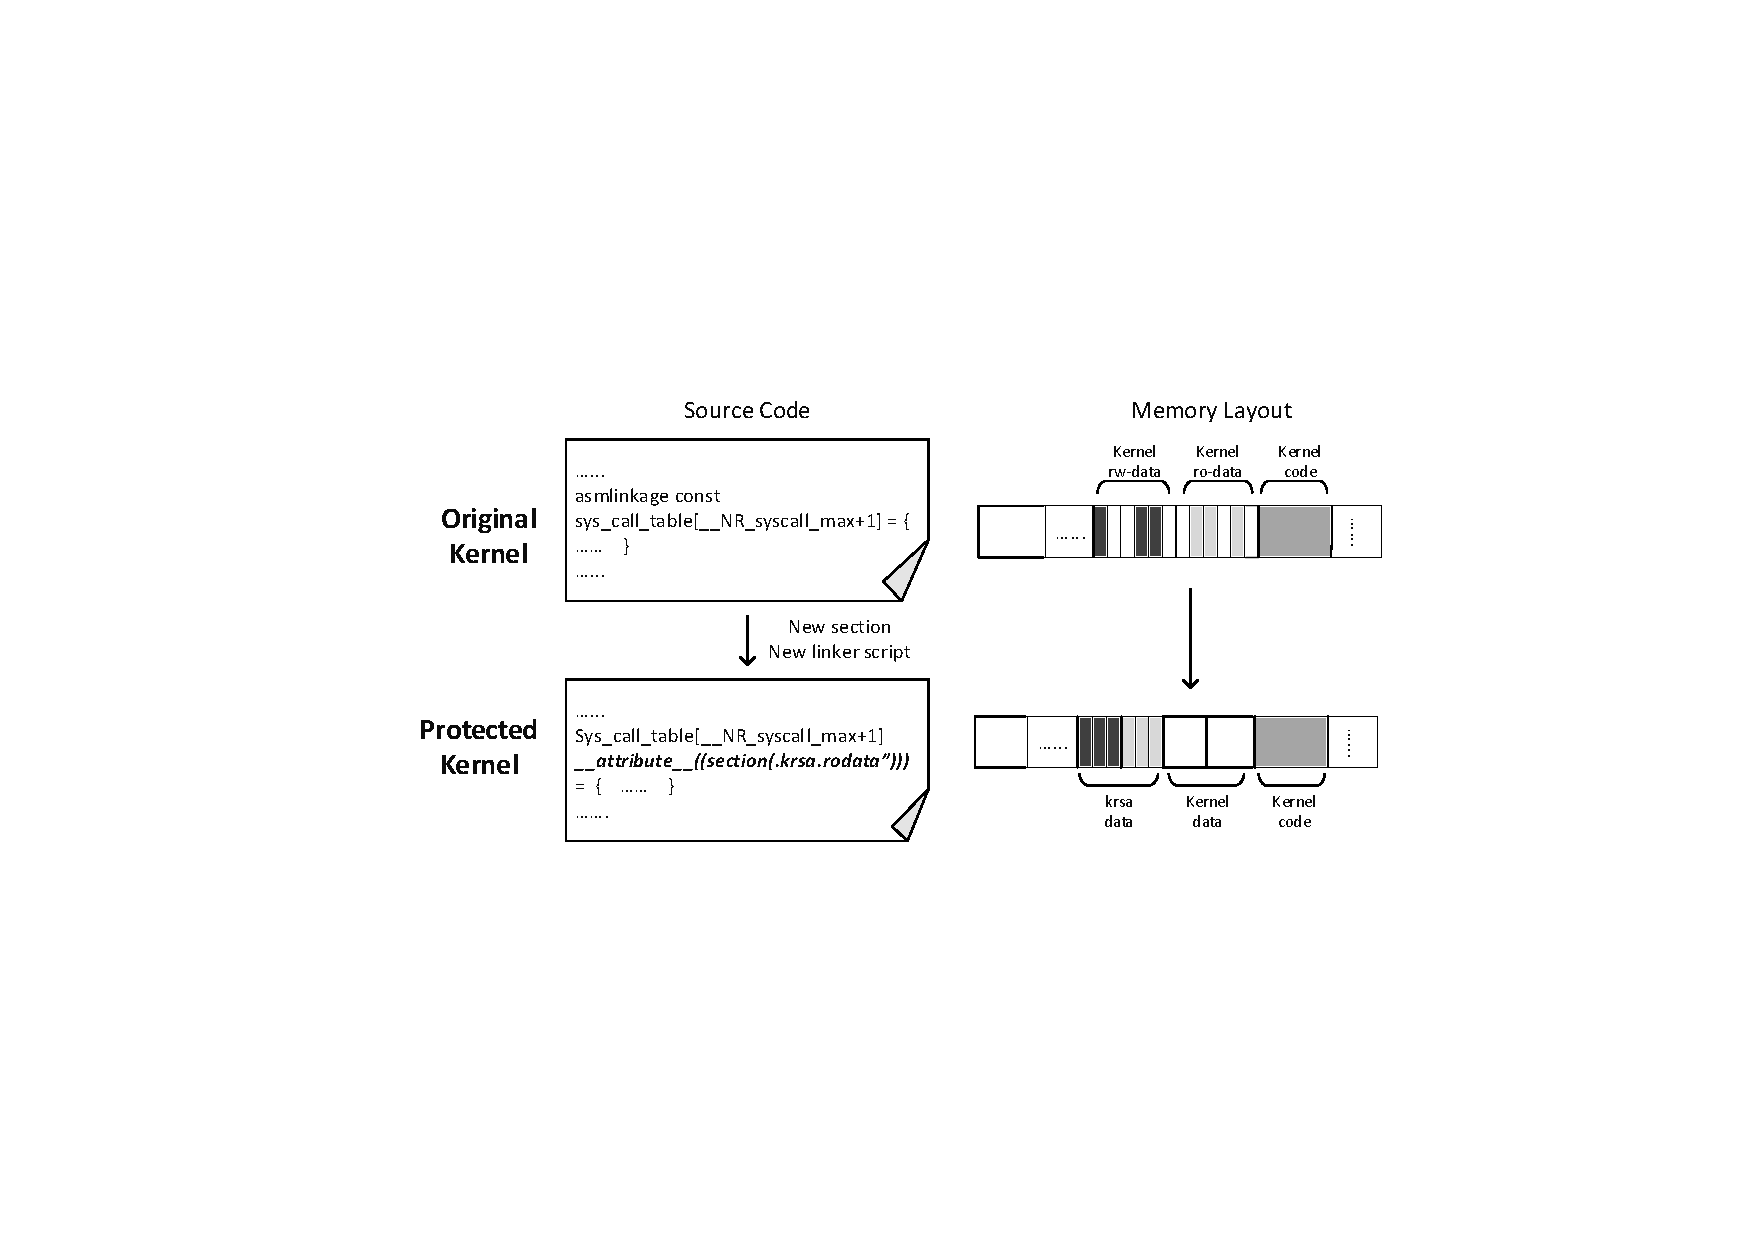
\includegraphics[scale=0.5]{pic/data_aggregate.pdf}
    \caption{Object Selection}
    \label{recompile}
\end{figure}
For example, system call table is one of the most important kernel data structures for the kernel security. In the real world, \textbf{adore} is one of the kernel rootkits that replaces the entry of 15 system calls with its own malicious function. The labeling procedure in KRSA, as depicted in Figure \ref{recompile}, 
adds a new section called \textbf{.krsa.rodata} in the source code to partition the kernel data structure layout
Then, KRSA requires to recompile the source code with a new \textbf{linker script}. Therefore, malicious or benign modifications to physical memory regions that contain critical kernel data structures can be observed and enforced at the hypervisor layer. 
Different kernel data structures need different protection requirements, labeling procedure in KRSA leverages kernel source code to distinguish different requirements and develops several \textbf{sections} to construct extensible protection purpose. 

% and then constructs the kernel heap graph to facilitate in understanding kernel malware behavior.
% extracts the memory management data structures from kernel source code.

% 引出首先handlerules是在source code定义数据结构的时候,由修改源代码的开发者定义的,其是一个json数据格式,这里给出一个数据格式的例子,并说明每个字段的意义。
% 然后当其被引入到krsa内部的时候,其地址字段会被替换为物理地址。
% 由虚拟地址到物理地址的映射过程涉及到页表的遍历,这部分涉及到页表的保护。由此引入页表的分类,哪类页表要保护什么样子的数据,对应的修改权限是什么,原因是什么。对于不同的页表,对应也会生成对应的页表的handlerules。
%
% 所有的上面的东西说完了,再说明这些操作还有具体的保护是由谁完成的,这时候涉及到两个引擎的。简要介绍这两个引擎的工作。 然后再介绍工作流程。

% HandleRule 的作用是什么?首先其是由开发者定义的数据结构,用于定义哪些数据结构需要保护,读写的权限是什么,若出错之后,对应的异常处理程序应该是怎么样的。
% 其次在KRSA读入该数据之后,其又是如何运作的?还是只是说这个数据用于后续KRSA内部使能??倾向于后者但是,如何写?因为不同字段是给不同的引擎使用的,如何写?
% 需要解释各个字段的含义,上面的内容都是可以在解释字段的时候说明,那么关键在于如何引入解释字段,首先要说明其作用。
% 其作用有两个,一个是给开发者使用,用于定义哪些数据需要保护,另外一个是在KRSA内部,其作用是什么?作为保护的依据。
Our second technique, HandleRule, is another technique to protect critical kernel data structures. HandleRules are high-level objects implemented on top of KRSA. Each HandleRule defines one critical kernel data structure to be protected by KRSA. HandleRules are written by the developer who modifies the source code using the method mentioned before. And, Figure \ref{hdrltemp} depicts the \textbf{JSON} template of a HandleRule. 

\begin{figure}[ht]
    \centering
    \begin{alltt}
{    \{"\textbf{Name}": "Data Name", 
    "\textbf{Address}": ADDR, "\textbf{EnableBit}": 1, 
    "\textbf{Permission}":010, "\textbf{HandleCode}":0x3F\}} \end{alltt}
\setlength{\abovecaptionskip}{0pt}
\setlength{\belowcaptionskip}{0pt}
\caption{HandleRule Template}
\label{hdrltemp}
\end{figure}

% \begin{figure}[ht]
%     \centering
%     \begin{verbatim}
%     {"Name": "Data Name",
%     "Address": ADDR, "EnableBit": 1,
%     "Permission":010, "HandleCode":0x3F} \end{verbatim}
% \setlength{\abovecaptionskip}{0pt}
% \setlength{\belowcaptionskip}{0pt}
% \caption{HandleRule Template}
% \label{hdrltemp}
% \end{figure}
In each HandleRule: 

\begin{itemize}
\item Name: This value indicates the name of the protected kernel critical data structure. The developer fills in this value, the content of which is the same as the corresponding data structure name in the modified source code. 
\item Address: This value indicates the address of the protected kernel critical data structure. This field does not require the intervention of the developer. It is automatically maintained by KRSA, and its value is different at different stages of KRSA, this will be elaborated in section \ref{sec:oledesign}. 
\item EnableBit: This value indicates whether this HandleRule is valid. 
\item Permission: This value determines what the kernel can and cannot do to this selected kernel data structure. 
\item HandleCode: This value indicates the predetermined actions to be executed when illegal access to protected kernel data structures occurs. These actions are fetched and executed by KRSA. 
\end{itemize}

In summary, KRSA monitors special memory regions registered by HandleRules, and triggers further actions when access that does not match the \textbf{Permission} value appears. On receiving the illegal access signal, KRSA fetches the \textbf{HandleCode} of the HandleRule. Then, KRSA triggers an action that corresponds to the pair of the \textbf{Address} and the \textbf{HandleCode} value. 
KRSA would catch every memory access operation to the protected memory regions. For this reason, the HandleRule should be written prudently so that access to the data structures will serve as an effective trigger to the protection mechanism in KRSA.

%保护页表的作用,一方面,页表的作用是因为其维护了虚拟到物理地址的映射,攻击者可以通过修改页表来实现对内存的任意操作,实施double map和remap攻击
\subsubsection{Page Table Protection} \label{sec:ptdesign}
Page tables are data structures that map virtual addresses to physical addresses. 
Page table entries describe the address mapping relationship and access permissions of each page. 
An attacker who is in control of page tables can launch various memory corruption attacks, such as remapping attacks and double mapping attacks. 
KRSA thwarts this attack by depriving the kernel with the capability of modifying corresponding kernel page tables. Since any update to protected page tables will be synced to physical memory region which are page tables located, the tiny hypervisor in KRSA verifies whether the update operation is illegal. If so, KRSA would forbid the update operation. 
% 因为页表索引的是不同的内容,因此对不同的页表项的保护是不同的。
% Depending on the memory content type that a page table entry decribes, as the Figrue \ref{pg} depicts, page table entries can be classified into five types:
Depending on the memory content type that a page table entry decribes, page table entries can be classified into five types: 
\begin{itemize}
\item Code-relevant PTE (E1), which involves mapping the kernel code. 
\item Data-relevant PTE (E2), which involves mapping the protected kernel data structures. 
\item Restricted PTE (E3), which shares the same page table with one or more page table entries that belong to Code-relevant PTE (E1).
\item Unrestricted PTE (E4), which shares the same page table with one or more page table entries that belong to Data-relevant PTE (E2), and in that page table, none of the page table entries belong to Code-relevant PTE (E1).
\item Unmonitored page PTE (E5), which belongs to a page table that none of page table entry in that page table belongs to any categories mentioned above. 
\end{itemize}
% 下面要讲为什么这么分类
%
% \begin{figure}
%     \centering
%     % 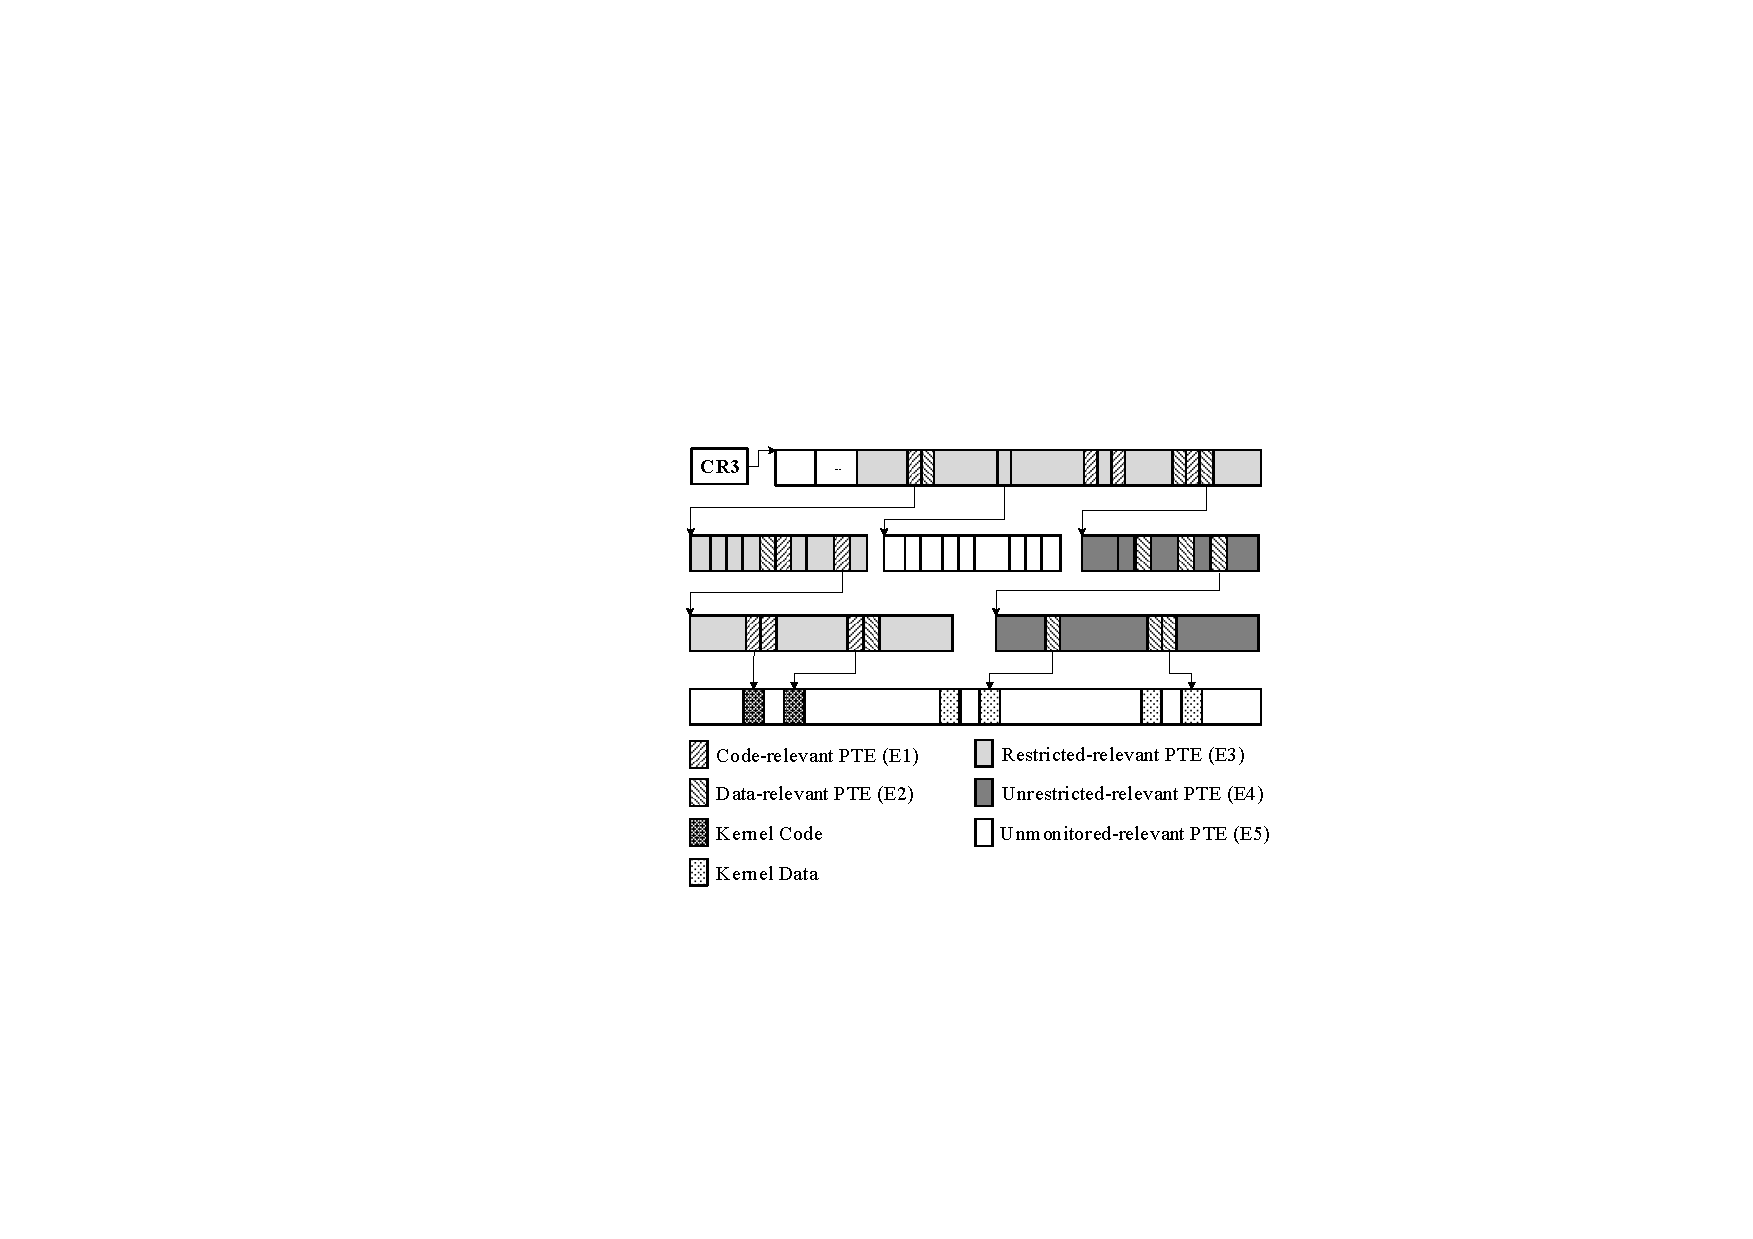
\includegraphics[scale=0.7]{pic/page_table.pdf}
%     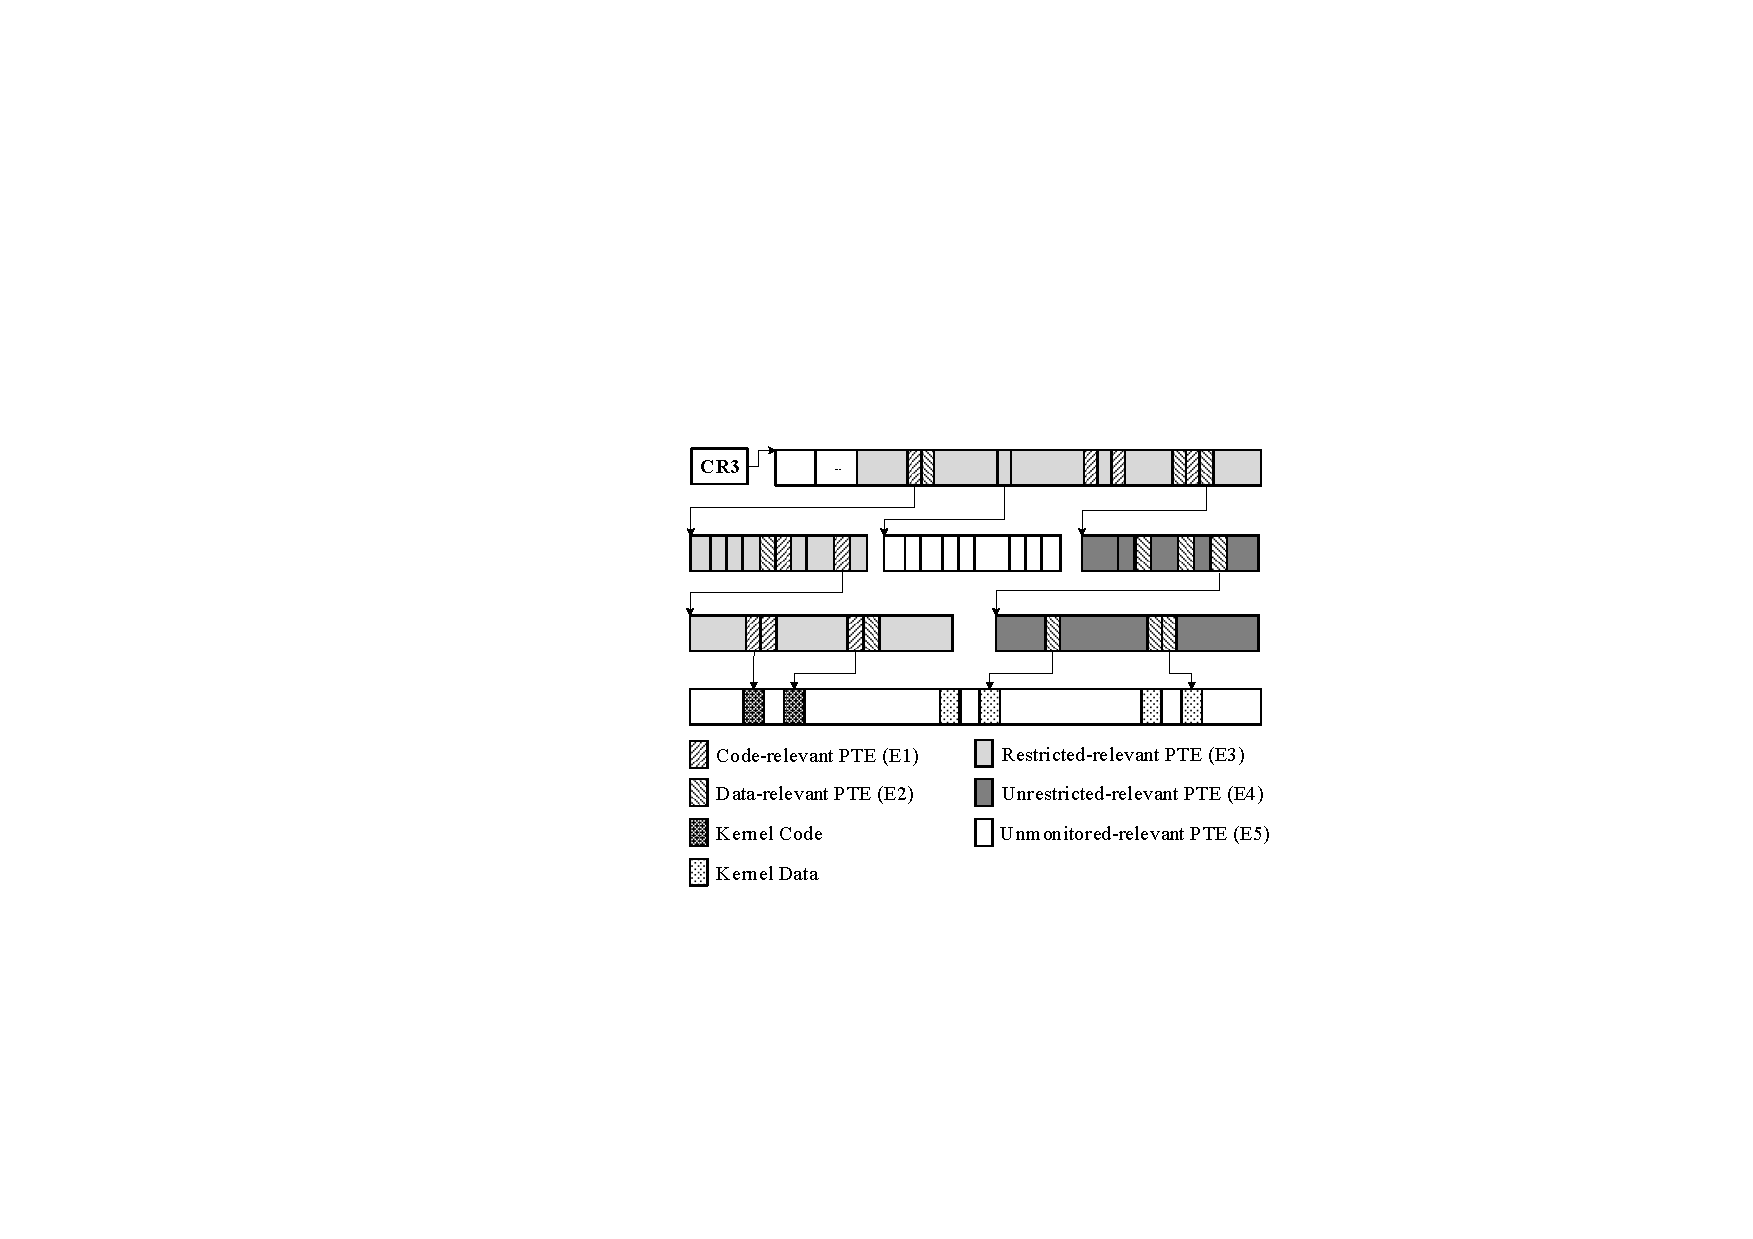
\includegraphics[width=7cm, height=5cm]{pic/page_table.pdf}
%     \caption{An Example of Page Table Entry Classification}
%     \label{pg}
% \end{figure}

Memory corruption attacks, especially remapping attacks and double mapping attacks, mainly subvert kernel code and the protected kernel data structures by assigning original virtual address to a new allocated physical address or mapping the protected physical address with a fake virtual address. To handle these cases, KRSA enforces two page table entries (E1 and E2) invariants. KRSA enforces that physical pages used for these critical page table entries can never be remapped, nor can their mapping (including access permissions) be modified. 
Another issue is about how to track other page table entries which locate in the same page table with them that belong to E1 or E2. Because the hypervisor can provide only page-level granularity, write operations to these page table entries (E3 and E4) would be trapped into the hypervisor too. In KRSA, we implemented an instruction write emulator inside the hypervisor to perform the emulation of these page table entry writes. More details about how KRSA emulates write the page table entry that belongs to E3 or E4 would be illustrated in section \ref{sec:pgimp}.

\subsection{KRSA Architecture} \label{sec:archdesign}
Figure \ref{arch} shows the architecture of KRSA. As shown in this figure, the hypervisor is the heart of KRSA's protection, comprised of Object Locating Engine, Object Protection Engine, LKM Protection Engine, and HandleRules. The Object Locating Engine includes a trusted driver used as a bridge between the hypervisor and the protected kernel, a trusted boot component used to init KRSA, and Object Locating Engine used to form HandleRules in KRSA. Object Protection Engine includes EPT Setting and Exception Handle. LKM Protection Engine includes Module Load, Module Unload and Integrity Measurement. HandleRule which corresponds to the HandleRule written by the developer is a data structure that used internally by KRSA to set protection for the protected kernel.

\begin{figure}
    \centering
    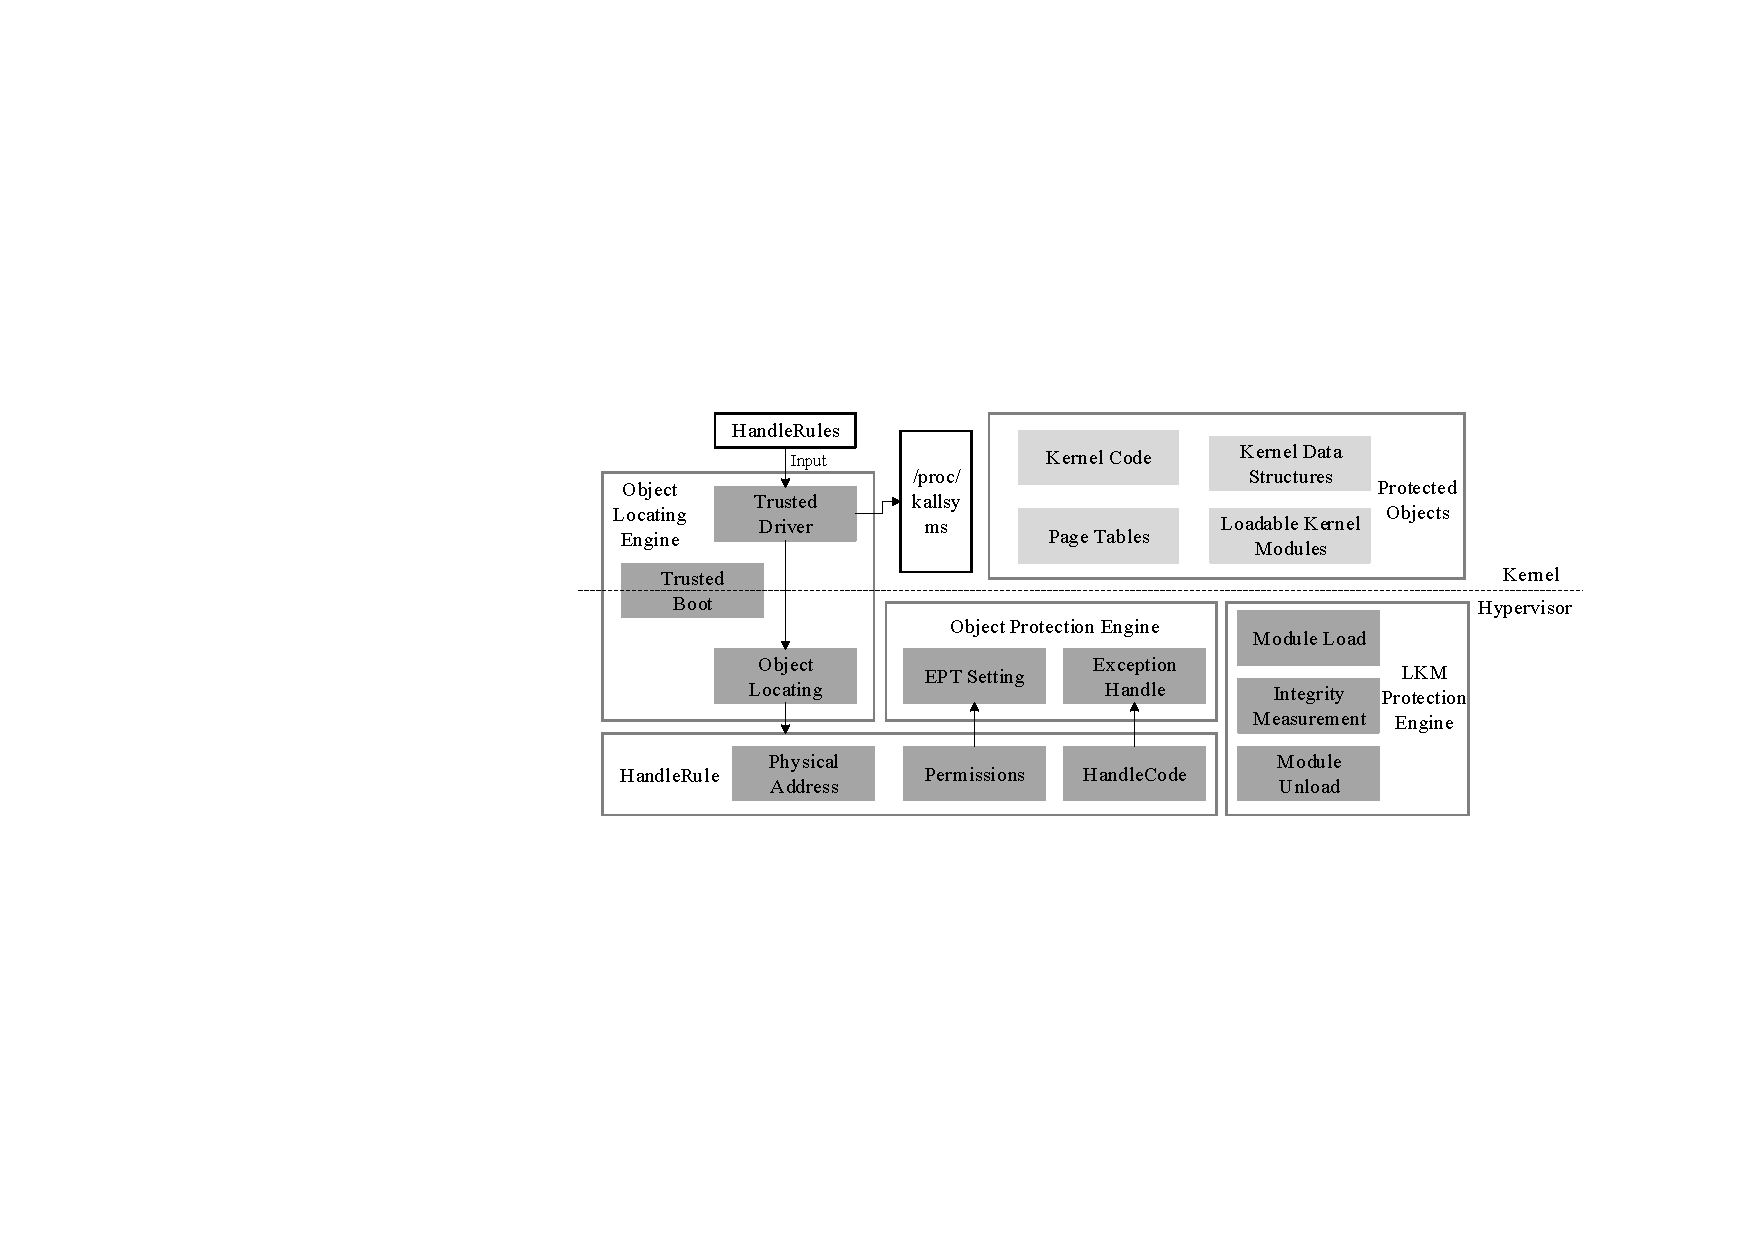
\includegraphics[scale=0.5]{pic/architecture.pdf}
    \caption{KRSA Architecture}
    \label{arch}
\end{figure}

\subsubsection{Object Locating Engine}\label{sec:oledesign}
Object Locating Engine is the core component that inits KRSA and converts user-input HandleRules into HandleRules used internally in KRSA. 
Trusted Boot is the first component that is initialized upon KRSA startup. It is responsible for allocating a contiguous physical memory block from the protected kernel and loading KRSA into memory. Trusted Boot component is also responsible for enabling hardware-assisted virtualization, setting up the tiny hypervisor, and a secure and safe switch between the protected kernel and the tiny hypervisor. This switch process would be illustrated in section \ref{sec:trustedboot}.
Trusted Driver is inserted into the protected kernel. It is responsible for notifying Object Locating component about the Address, Permissions, and HandleCode of each HandleRule. The Trusted Driver component read all HandleRules configuration files in \textbf{JSON} template and refers to \textbf{/proc/kallsyms} to obtain the location of each protected data structure. This driver then communicates with Object Locating component to pass all HandleRules through \textbf{Hypercall}.
Object Locating is responsible for walking the host page tables to perform virtual to physical address translation of each HandleRule. At this stage, the hypervisor has been already initialized, the Object Locating component could accomplish this translation without any help of the protected kernel. 
It would also formulate HandleRules about the related page table entries during the procedure of walking the page tables.


\subsubsection{Object Protection Engine} \label{sec:opedesign}
Object Protection Engine is the main component of the tiny hypervisor in KRSA, enabling the memory access protection mechanism.
With the help of virtualization technology, accesses to physical memory pages are subject to permission checks in both Extended Page Tables (EPT) in the hypervisor and protected kernel page tables. 
Any update to the protected memory region is trapped and propagated to the EPT by the hypervisor, In other words, the hardware performs the address translation with the result of EPTs and kernel page tables. Thus, KRSA uses EPT as the basis of its hardware memory protections.
EPT Setting component is responsible for setting EPT entries' permissions upon the registration of HandleRules. Exception Handle component is responsible for fetching the HandleCode in HandleRule and executing the predetermined actions when illegally memory access occurs. 
The category of exceptions consists of kernel code, kernel data structure, page table, and kernel self-modifying code. 
Besides, considiering a mixed page that has kernel data and kernel code, different page table entries, the hypervisor would trap all accesses that modify this page. Then KRSA examines the pair of the virtual and physical address to see if it is matched with a HandleRule and finally determines the following action. Figure \ref{pic:excep} depicts the exception handle routine of KRSA. 

\begin{figure}
    \centering
    % 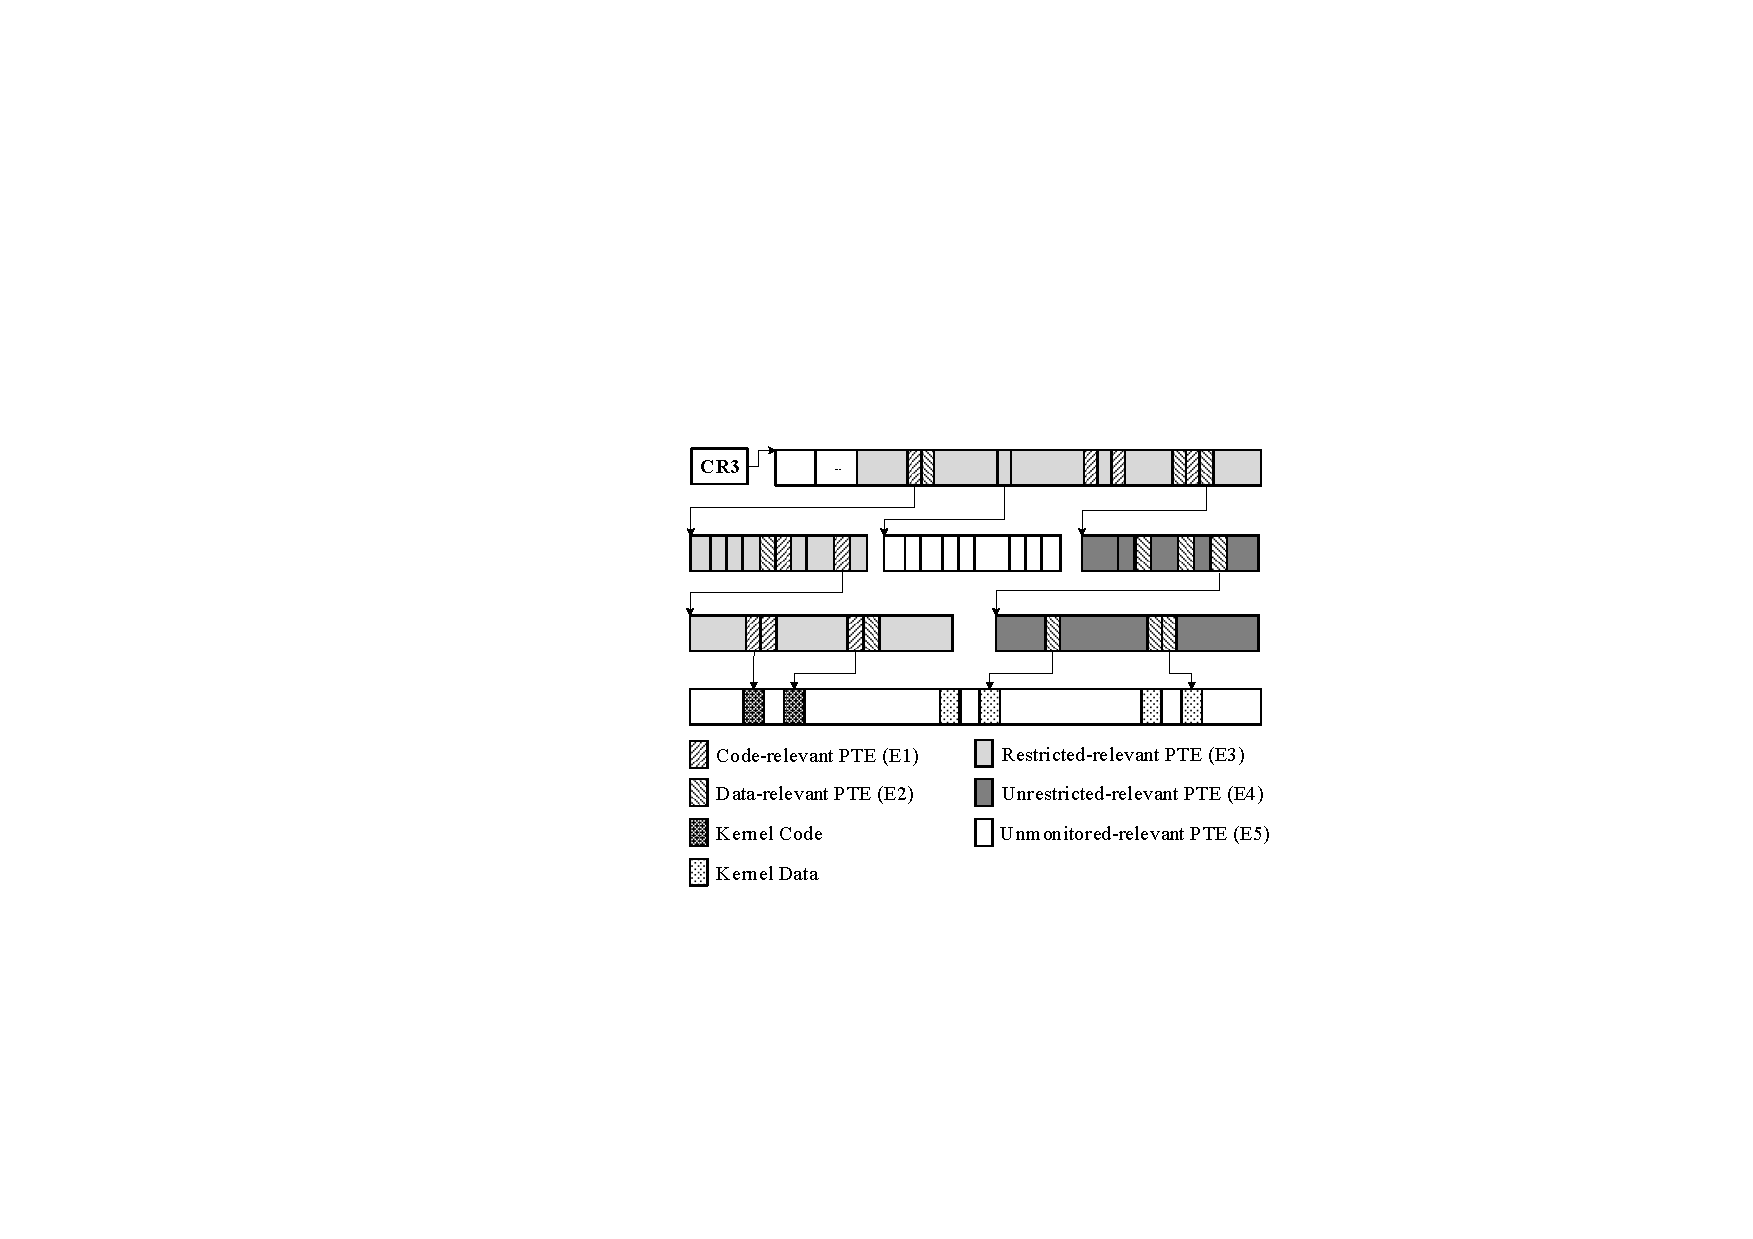
\includegraphics[scale=0.7]{pic/page_table.pdf}
    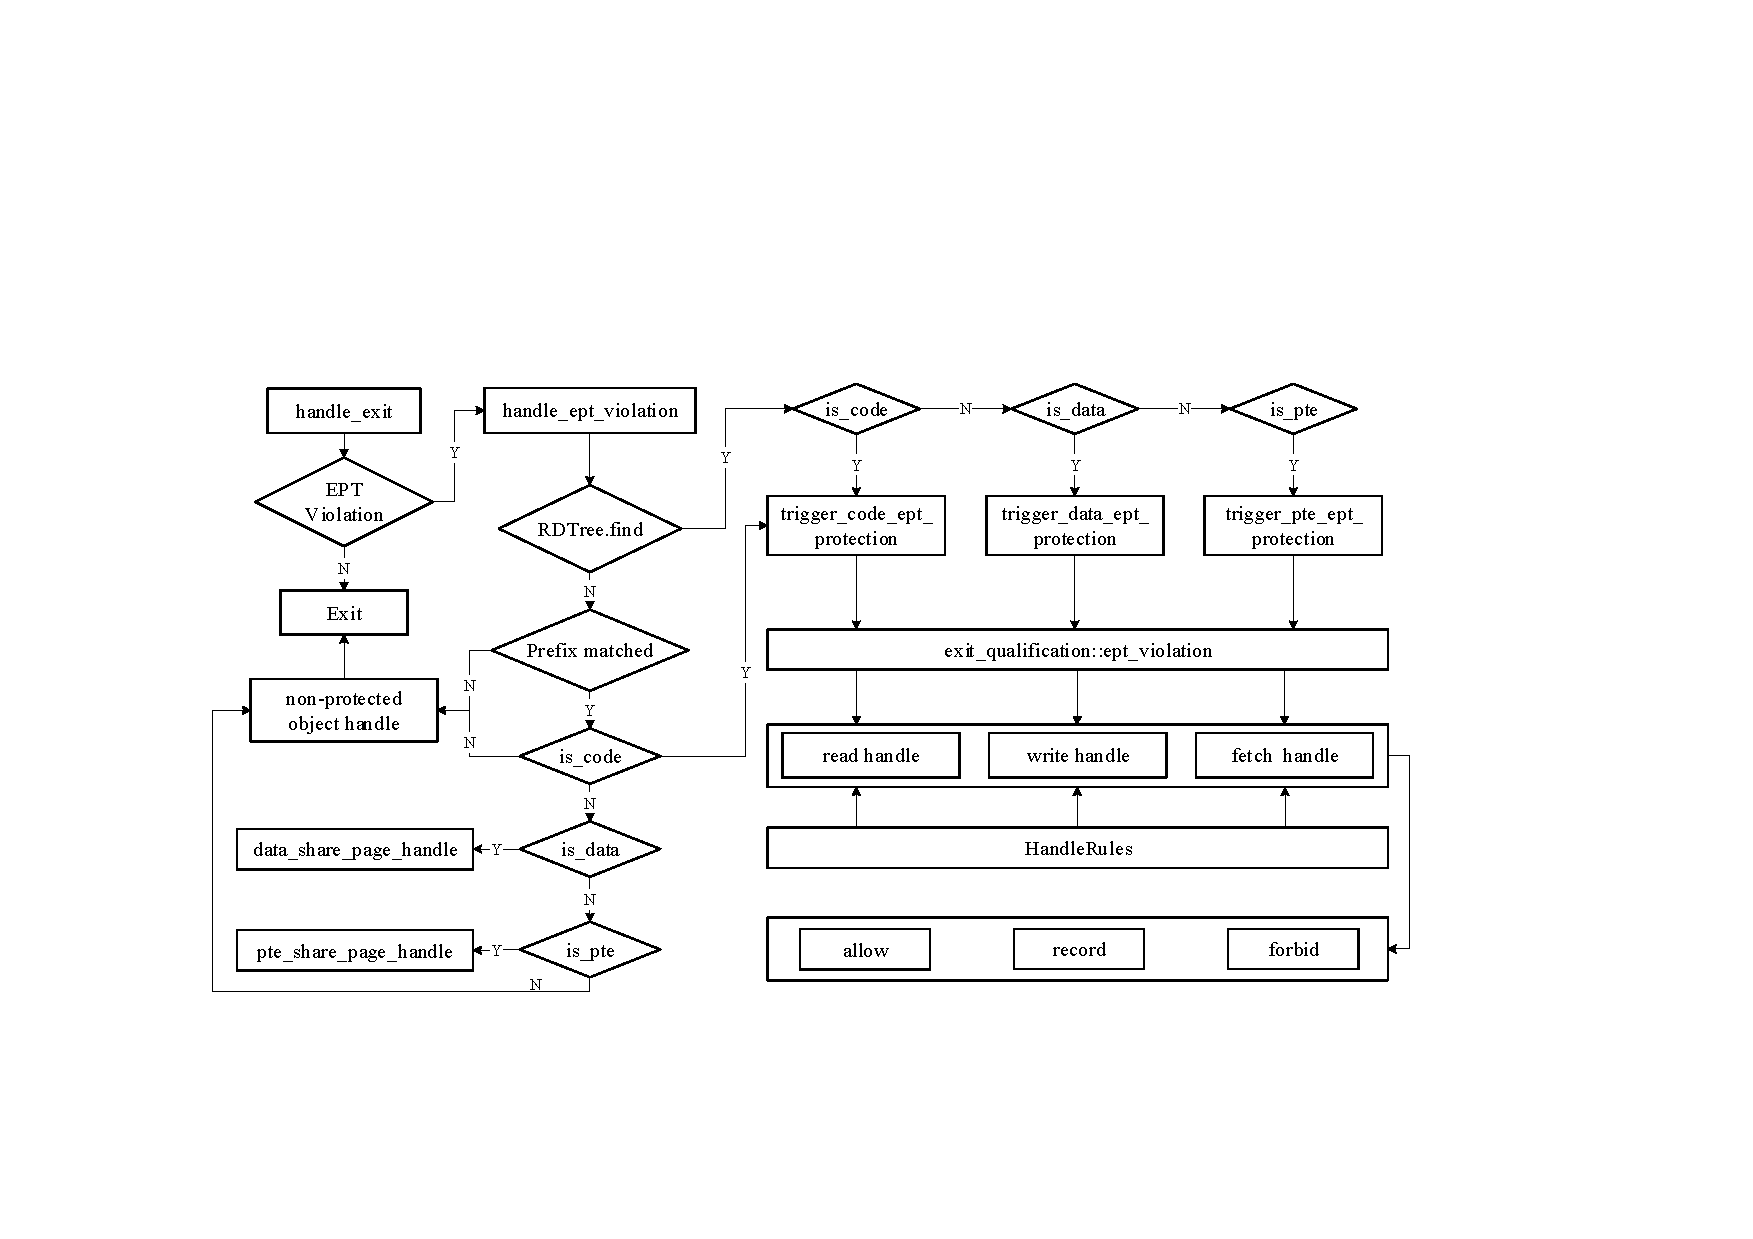
\includegraphics[width=7cm, height=3.5cm]{pic/exception.pdf}
    \caption{Exception Handle Routine in Object Protection Engine}
    \label{pic:excep}
\end{figure}

\subsubsection{LKM Protection Engine}\label{sec:lkmdesign}
LKM Protection Engine is introduced to handle loadable kernel module protection. This engine is compromised of three components: Module Load, Module Unload and Integrity Measurement. 
Firstly, Integrity Measurement is performed on receiving the signal that the protected kernel is going to load a new loadable kernel module, this step would ensure that the newly introduced modules are authorized modules. Secondly, LKM Protection Engine would interface with Object Locating Engine after an LKM is loaded into memory. This engine delivers the information, such as where the module code is loaded and where the data that needed to be protected is, to Object Locating Engine. Loadable kernel module actually is loaded and executed with kernel privilege, so KRSA must take the newly introduced kernel module code and data into consideration, especially when the user defines some data structures to be protected in the newly introduced kernel module. 



% 设计部分,图重新画
% 实现部分的内容,主要是针对上面设计部分提到的具体如何保护的实现,对于数据的标记再详细说明,说明链接脚本。主要包括如何保护内核代码,处理自修改代码的具体的方法,页表的保护方法,页表的写模拟,如何可信启动等内容
% 要写页表保护,即页表对于E3 E4是如何保护的,主要内容应该是写模拟,如何模拟对他们的写操作的。
\section{Implementation} \label{sec:imp}
We decided to prototype KRSA for ArchLinux with kernel 4.2.5. 
Our design as presented in Section \ref{sec:design} requires source code modifications to the operating system kernel, and requires recompilation with a new linker script.
To this end, our kernel patch is 37 SLOC modifications, and the tiny hypervisor is 3251 SLOC. 
In this section, we will discuss specific implementation details. Figure \ref{pic_imp} depicts how the prototype of KRSA alters the kernel memory layout to aggregate data needing the same policy enforcement on the same memory pages. This figure also depicts how KRSA handles exceptions when illegal access occurs. 

\subsection{Object Marking} \label{sec:objmarkimp}
As mentioned earlier, KRSA develops several new sections for different protection purpose. The labeling procedure in KRSA needs to specify the protected data structure manually and recompile the kernel source code with a new linker script. In our prototype, there are, currently, two new sections: \verb|.krsa.data| and \verb|.krsa.rodata|.
The hypervisor mediates the execution of write memory accesses to the data with label \verb|.krsa.data|. For these data, KRSA protects the data from being modified by any entity but KRSA and its TCB. For other data structures with label \verb|.krsa.rodata|, KRSA forbids any write operation to them. 
The import of new sections provides freedom in laying out the protected and unprotected data structures in memory at runtime, though it needs kernel source code revision. This process has only a minimal source code change to the definition of the structure. 
% Figure \ref{secexample} gives an example on this process.
% \begin{figure}[ht]
%     \centering
%     \begin{alltt}
% {   // security/security.c
%     ...
%     struct security_hook_heads
%     security_hook_heads
%     __attribute__
%     ((section (".ckrsa.data"))) = {...}  } \end{alltt}
% \setlength{\abovecaptionskip}{0pt}
% \setlength{\belowcaptionskip}{0pt}
% \caption{A Section Attibute Example}
% \label{secexample}
% \end{figure}
\begin{figure}
    \centering
    % 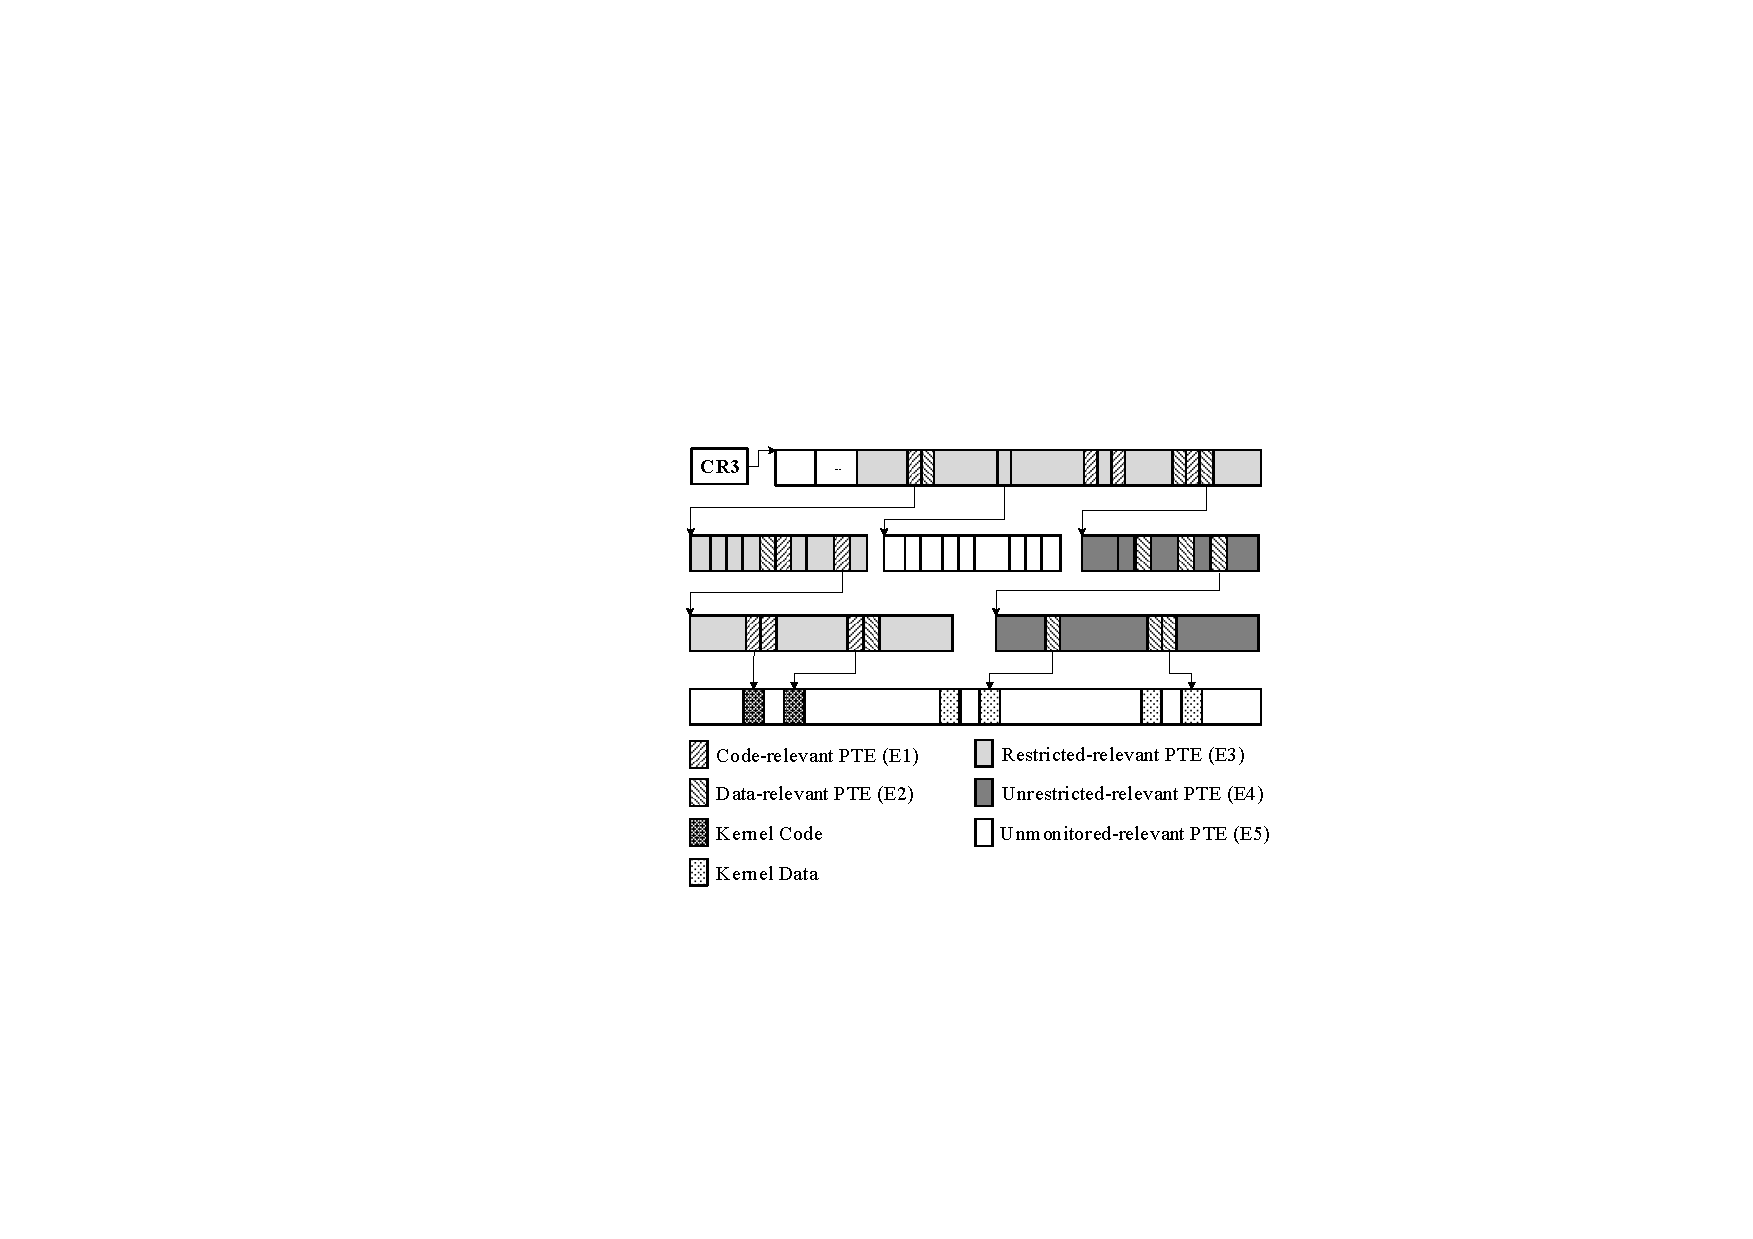
\includegraphics[scale=0.7]{pic/page_table.pdf}
    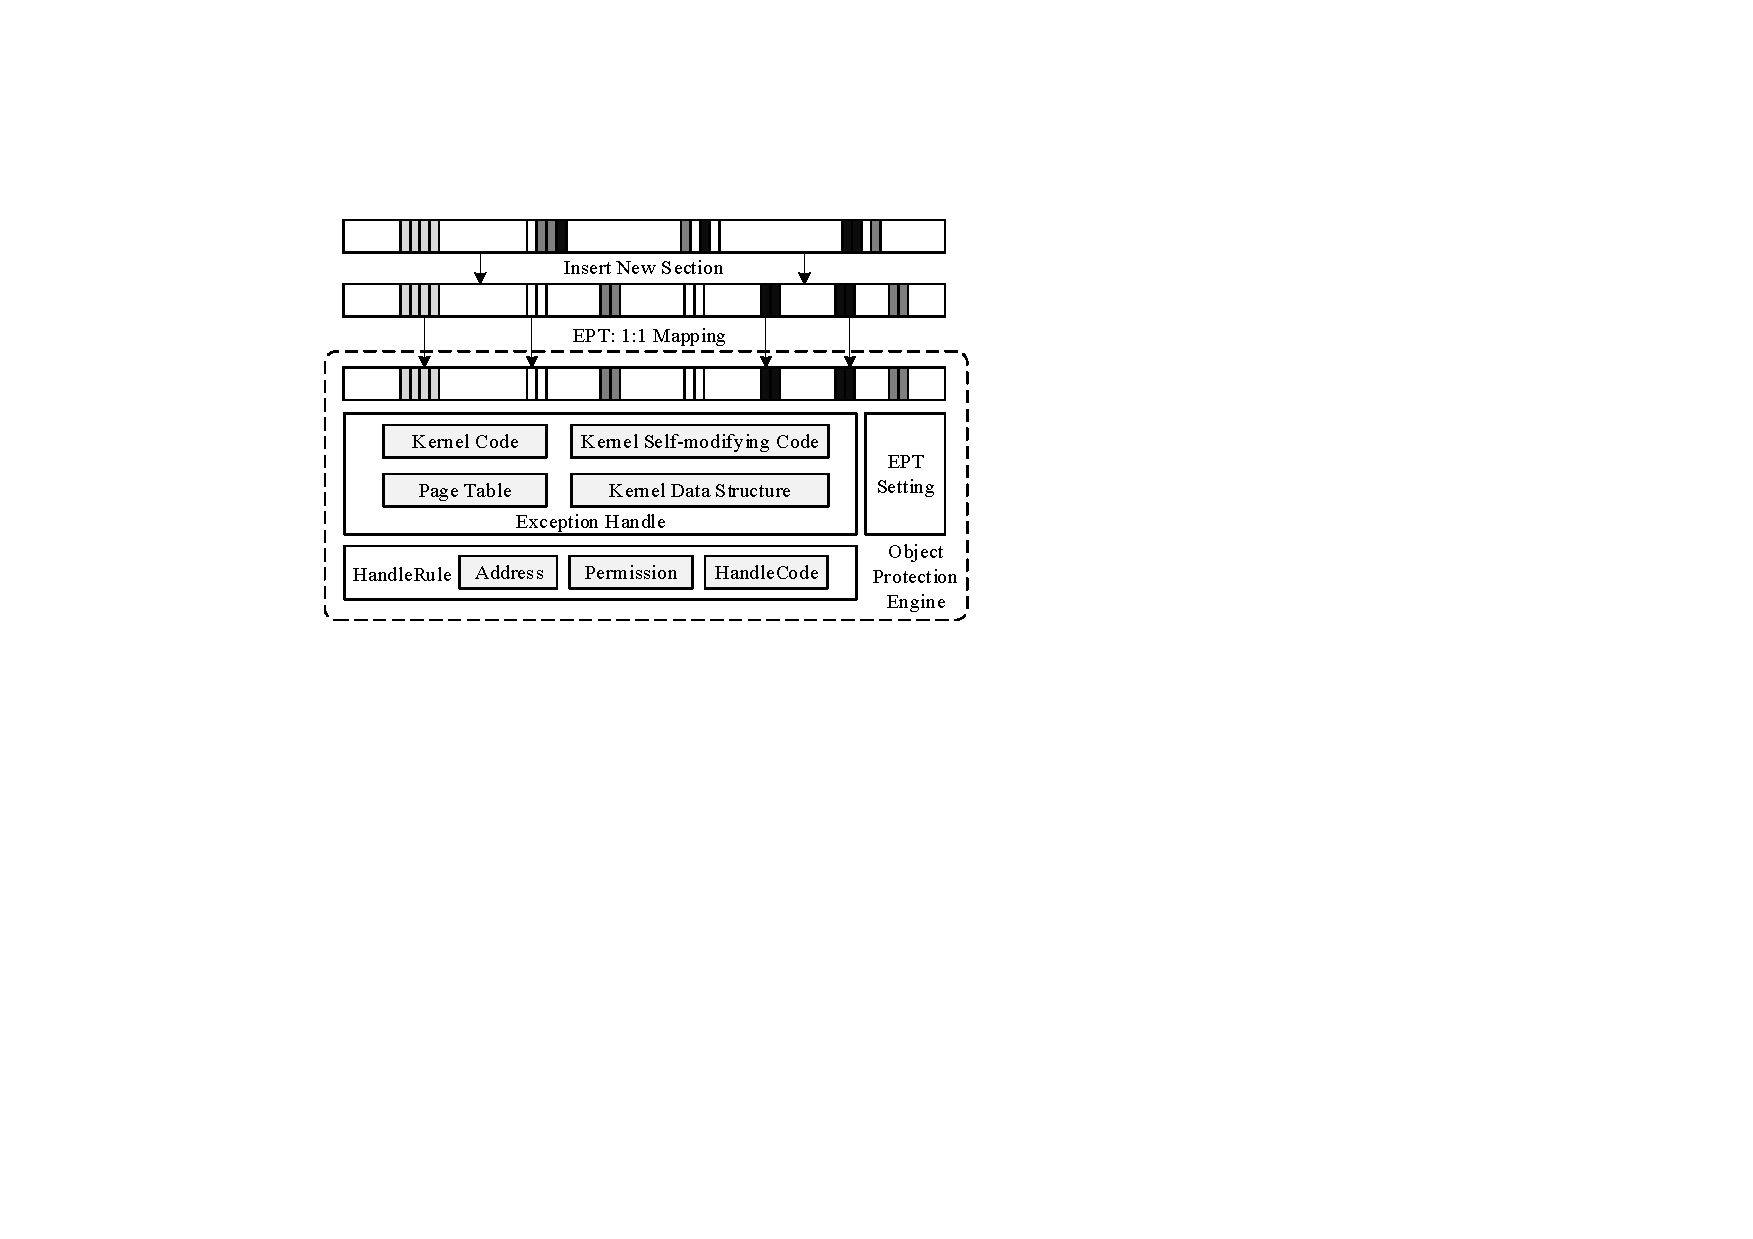
\includegraphics[width=8cm, height=4cm]{pic/imp.pdf}
    \caption{Memory Layout and Runtime Exception Handle}
    \setlength{\abovecaptionskip}{0pt}
    \setlength{\belowcaptionskip}{0pt}
    \label{pic_imp}
\end{figure}


A modified linker script is used to aggregate data at compile time. It aggregates data structures that process the same permission into the same physical memory page. Though this may not be an effective use of kernel memory, and it imposes constraints on runtime memory layout, it actually benefits more for the memory protection in the hypervisor. Figure \ref{linkerexample} gives an example of a modified linker script. 
\begin{figure}[ht]
    \centering
    \begin{alltt}
    {// arch/x86/kernel/vmlinux.lds.S
    /* Data */
    . = ALIGN(PAGE_SIZE);
    .krsa.data : 
    AT(ADDR(.ckrsa.data) - LOAD_OFFSET)
    \{ *(.krsa.data) \} } \end{alltt}
\setlength{\abovecaptionskip}{0pt}
\setlength{\belowcaptionskip}{0pt}
\caption{A Modified Linker Script Example}
\label{linkerexample}
\end{figure}


\subsection{Kernel Code and Kernel Self-modifying Code} \label{sec:codeimp}

\subsubsection{Kernel Code Exception Handle} \label{sec:subcodeimp}
As mentioned earlier, KRSA mainly protects kernel code with Code Integrity Policy. In our prototype, Object Protection Engine monitors and rejects any write operation to these memory ranges containing kernel code. Object Locating Engine removes the write permission in each page table entry that associates with kernel code. Meanwhile,  Object Protection Engine reinforces this policy in associated EPT entries. Thus, when the adversary attempts to subvert kernel by modifying kernel code, Object Protection Engine would always capture this operation and reject it with the help of tiny hypervisor. 
In addition, Object Protection Engine also prevents the adversary from adding or deleting code, this work is accomplished by protecting page table entries that belong to E1 and E3. More details about how KRSA handles illegal access to these page table entries would be illustrated in section \ref{sec:pgimp}. 

\subsubsection{Kernel Self-modifying Code Exception Handle} \label{sec:subselfcodeimp}
At runtime, some kernel features leverage self-modifying code. These features, obviously, break Code Integrity Policy. Object Protection Engine needs to handle these exceptions additionally. 
% In general, kernel codes aren't alternated during runtime. However, there are some kernel features actually modifying kernel codes at runtime.
% So KRSA adopts special HandleRules to deals with these codes. At runtime, any modification to kernel code would force virtual machine exit, and Object Protection Engine would search all HandleRules to find out whether the VM-Exit matches a kernel self-modifying code`s HandleRules or not. In our prototype, KRSA formulates four kind of HandleRules for different kind of Kernel Self-modifying Code.

Static Keys is used for less branch prediction. When kernel code is modified, in the handler to this kind of kernel self-modifying code, KRSA would force Object Protection Engine to check if a code address in an array named \textit{jump\_entry} matches the address of the modified instruction. If matches, Object Protection Engine would authorize the operation of this instruction.  


% Static Keys swaps between \verb|NOP| instruction and \verb|JUMP| instruction to switch branches instead of condition instructions for less branch predictions. KRSA forces Object Protection Engine to search an array of \textit{jump\_entry} structure which contains the address of the code which could be modified for a jump entry matching the address of the modified instruction. If Object Protection Engine doesn't find it, Object Protection Engine regards the modification isn't caused by this feature, which would trigger further another HandleRules to check or reject this operation. Swapping instructions is a complex process which needs the involvement of INT3 instruction, so Object Protection Engine defines a state machine to judge each step. According to the current instruction and the modification, Object Protection Engine gets a state and a state transition. If the transition doesn't satisfy the requirement of state machine, Object Protection Engine regard the step is illegal. Moreover, for a modification to \verb|JUMP| instruction, Object Protection Engine compares the instruction target and the jump target indicated by the jump entry. If they doesn't match, Object Protection Engine regards the modification is illegal.

KGDB would replace an instruction with \verb|INT3| to set a breakpoint when an instruction is replaced with \verb|INT3| instruction, Object Protection Engine would record the original bytes. When \verb|INT3| instruction is modified, Object Protection Engine would check if the address of this modification is recorded before, if not, Object Protection Engine would regard that operation illegal. 

% KGDB is a kernel debugger which replaces original instructions with the \verb|INT3| instruction to set breakpoints. KRSA allows modification to the \verb|INT3| instruction and just records original bytes and the addresses of the modifications. When \verb|INT3| instructions are modified, Object Protection Engine retrieves the records. If Object Protection Engine doesn't find a record where the address and the byte match the address and the byte of the modification, Object Protection Engine regards that operation is illegal.

Ftrace is an internal tracer which alternates the instructions at the beginning of functions. Object Protection Engine interfaces with Object Protection Engine retrieves the kernel symbol table to judge whether the modification is at the beginning of functions. 
% The same with Statc Keys, Object Protection Engine defines a state machine to judge the steps of swapping between \verb|NOP| instructions and \verb|CALL| instructions. The targets of \verb|CALL| instructions include some tracer functions which Object Protection Engine find according source code analysis and trampoline functions. The trampoline functions are dynamically generated depending on a function template. And the difference between them is a jump address in the end. So Object Protection Engine compares the trampoline function and the function template to ensure only the jump target is different and the target is one of functions which Object Protection Engine finds according to source code analysis.

Kprobes uses the INT3 instruction and Ftrace to change the control flow for collecting information.
In generally, Kprobes only uses \verb|INT3| instructions like the way KGDB uses. So Object Protection Engine adopts the same check method with KGDB\@. What's more, Kprobes has an optimizer which replaces \verb|INT3| instructions with JUMP instructions, so Object Protection Engine does checks like what it does in Ftrace. 
% does checks like what it does in KGDB\@. What's more, Kprobes has an optimizer which replaces \verb|INT3| instructions with JUMP instructions. The jump targets are also some trampolines, so Object Protection Engine does checks like what it does in Ftrace\@.

Alternatives alternate codes according to features of processors at runtime. All code modifications caused by the feature rely on another data structure. Fortunately, these modifications are done at boot time of the kernel, so it's unnecessary for KRSA to check them.
% KRSA doesn't support BPF too, because BPF introduces userspace codes, KRSA can't judge whether the modification is malicious or not. Fortunately, BPF is usually used in packet filter. Furthermore, if \verb|KGDB| \verb|Kprobes| and \verb|Ftrace| are not supported in practical scenario, KRSA may turn off  relevant protection mentioned above.

% 这部分主要写如何保护页表,主要是对E1到E4的页表是如何处理的进行详细说明,此外还有关键的模拟写的操作。
\subsection{Page Table Protection} \label{sec:pgimp}
As mentioned earlier, kernel page table entries are classified into five categories, KRSA deprives the kernel with the capability for modifying PTEs that are classified to be E1 to E4. The Object Protection Engine clears the write permission to the physical pages that contain protected PTE. Any write access to these PTEs would be trapped into the hypervisor, Object Protection Engine would check if there are any HandleRule matches the pair of the virtual and physical address. Then, this engine fetches the corresponding \textbf{HandleCode} and executes the predefined action. 
%页表的保护,需要在后面详细使用。
For PTEs that are marked to be E1, they are involved with address translation of the kernel code. KRSA needs to guarantee that the adversary can not subvert these PTEs by replacing kernel code with an unauthorized one. During the page table walking procedure in initialization, HandleRules for these PTEs require the Object Protection Engine to reject write access to these PTEs at the hypervisor level. 
% If someone tries to write a PTE marked to as E1, Object Protection Engine would force virtual machine exit and reject that operation with the help of tiny hypervisor.
For PTEs that are marked as E3, they should be considered because these PTEs share the same page with PTEs belonging to E1. KRSA must prevent an adversary from converting a data page to a kernel code page. 
% Unfortunately KRSA doesn't know the information of processes, it can't know whether a page is used as a code page or a data page, so KRSA can't limit the execution of pages.
% KRSA set the NX bits in the kernel page table entries whose level is as high as possible. Because once the NX bit is set in any level page table entries, the related page can't be executed anymore in the multiple level paging structure. These PTEs actually belong to E3.
Thus Object Protection Engine would reject the operation that if this operation adds execution permission to this type of PTEs or change the NX bit in page table permission field. For these safe write accesses, Object Protection Engine would emulate this write operation. The write emulation would be described in details in the following paragraph. 
% Thus when write operation to E3 occurs, Object Protection Engine forces virtual machine exit and checks if this operation adds execution permission to that PTE or change NX bit.
For PTEs that are marked as E2, they are involved with the address translation of the protected kernel data structures. Object Protection Engine rejects modification to the memory regions that contain PTEs who belong to E2. This guarantees the mapping relationships invariable to prevent the adversary from modifying these data structures illegally or replacing them with a fake one.
The PTE that belongs to E4 is protected because it shares the same physical page with the PTE that belongs to E2, so Object Protection Engine would be triggered and emulate the write operation if a PTE that belongs to E4 is written. 

Because the hypervisor can provide only page-level granularity, write accesses to PTEs that belong to E3 and E4 are trapped into the hypervisor too, Object Protection Engine has to emulate these write accesses. We observe that the modification to these page table entries behaves like assigning a new value to a memory address with a pointer. Thus, KRSA implements the write emulation with a fixed assembly code formation. \verb|mov| and \verb|movsb| are the two instructions that the Object Protection Engine emulates. In details, KRSA emulates the write operation by writing the value in a register into the memory region via register indirect addressing without offset. The value in register \verb|rcx| is used to determine the number of bytes to be written. 



\subsection{Loadable Kernel Module} \label{sec:lkmimp}
Loadable Kernel Module is a special case should be protected because it can introduce new kernel code and data structures. 
In details, KRSA mediates the load and unload process of the LKM through inserting two \verb|hypercall| into the kernel source code. 
% As a result, the LKM Protection Engine in the tiny hypervisor would be notified when the
% implements two hypercalls to deal with the addition and reduction of LKM code. By modifying the kernel source code, hypercall would be called if the protected kernel is going to load or unload a kernel module. In KRSA, LKM Protection Engine would receive these hyeprcalls to accomplish load and unload work in hypervisor.
At the time when the LKM initialization function is called, the LKM Protection Engine in the tiny hypervisor is notified to verify the integrity of the core text.
% and initialization text of the module before the kernel module initialization function at the time protected kernel is going to load a kernel module.
Then, LKM Protection Engine would inform Object Locating Engine to modify the permission of the last level page table entries of module regions, KRSA deprives these page table entries with execution permission. In this step, the LKM Protection Engine has not to load LKM core code into kernel space. This step mainly prevents the attacker from executing data pages. Thirdly, LKM Protection Engine loads LKM code into kernel space and forces Object Locating Engine to modify the kernel page table entries to restore the lost execution permission and correct the execution permission in high level page table entries. Object Locating Engine also constructs corresponding HandleRules just as the engine does for original kernel code.  
Data structures introduced by LKM is protected with similar steps. 
% If the developer want to protect some data structures imported by this LKM, developer just formulates the customizable HandleRules, then KRSA would load these HandleRules and protect these specified data structure.
On receiving the second hypercall, LKM Protection Engine would interface with Object Locating Engine to clear all execution permissions of the kernel PTEs which are related to the unloaded codes. This prevents any succeed execution of the module code.


\subsection{Trusted Boot} \label{sec:trustedboot}
% Because KRSA mainly focuses on runtime protection, and with the help of Intel TXT\cite{txtintel}, KRSA does not involve the boot process of the protected kernel. However, when the kernel initialization is completed, KRSA will be loaded as the first loadable kernel module, therefore, KRSA must ensure its own trusted boot.
At security environment, the Linux kernel usually is trusted boot with the help of TPM, because KRSA aims at providing the runtime protection, it does not interface with the boot process of the kernel. When the kernel initialization is completed, KRSA will be loaded as the first loadable kernel module, init the virtualization environment, and convert the protected kernel into a VM. During this process, KRSA must ensure its own security through trusted booting.
% KRSA provides runtime systematical protection to the customized kernel, thus KRSA does not involve the boot process to protect the kernel, actually, as described in Section \ref{section:frame}, KRSA would be the first kernel module to loaded after the kernel boot, thus KRSA must be loaded with trust.
% In order to ensure that KRSA can be loaded with trust, Object Locating Engine implements the loading process as shown in Figure \ref{db}.
% Figure \ref{pic_boot} depicts how KRSA boots itself with security guarantee.
% \begin{figure}
%     \centering
%     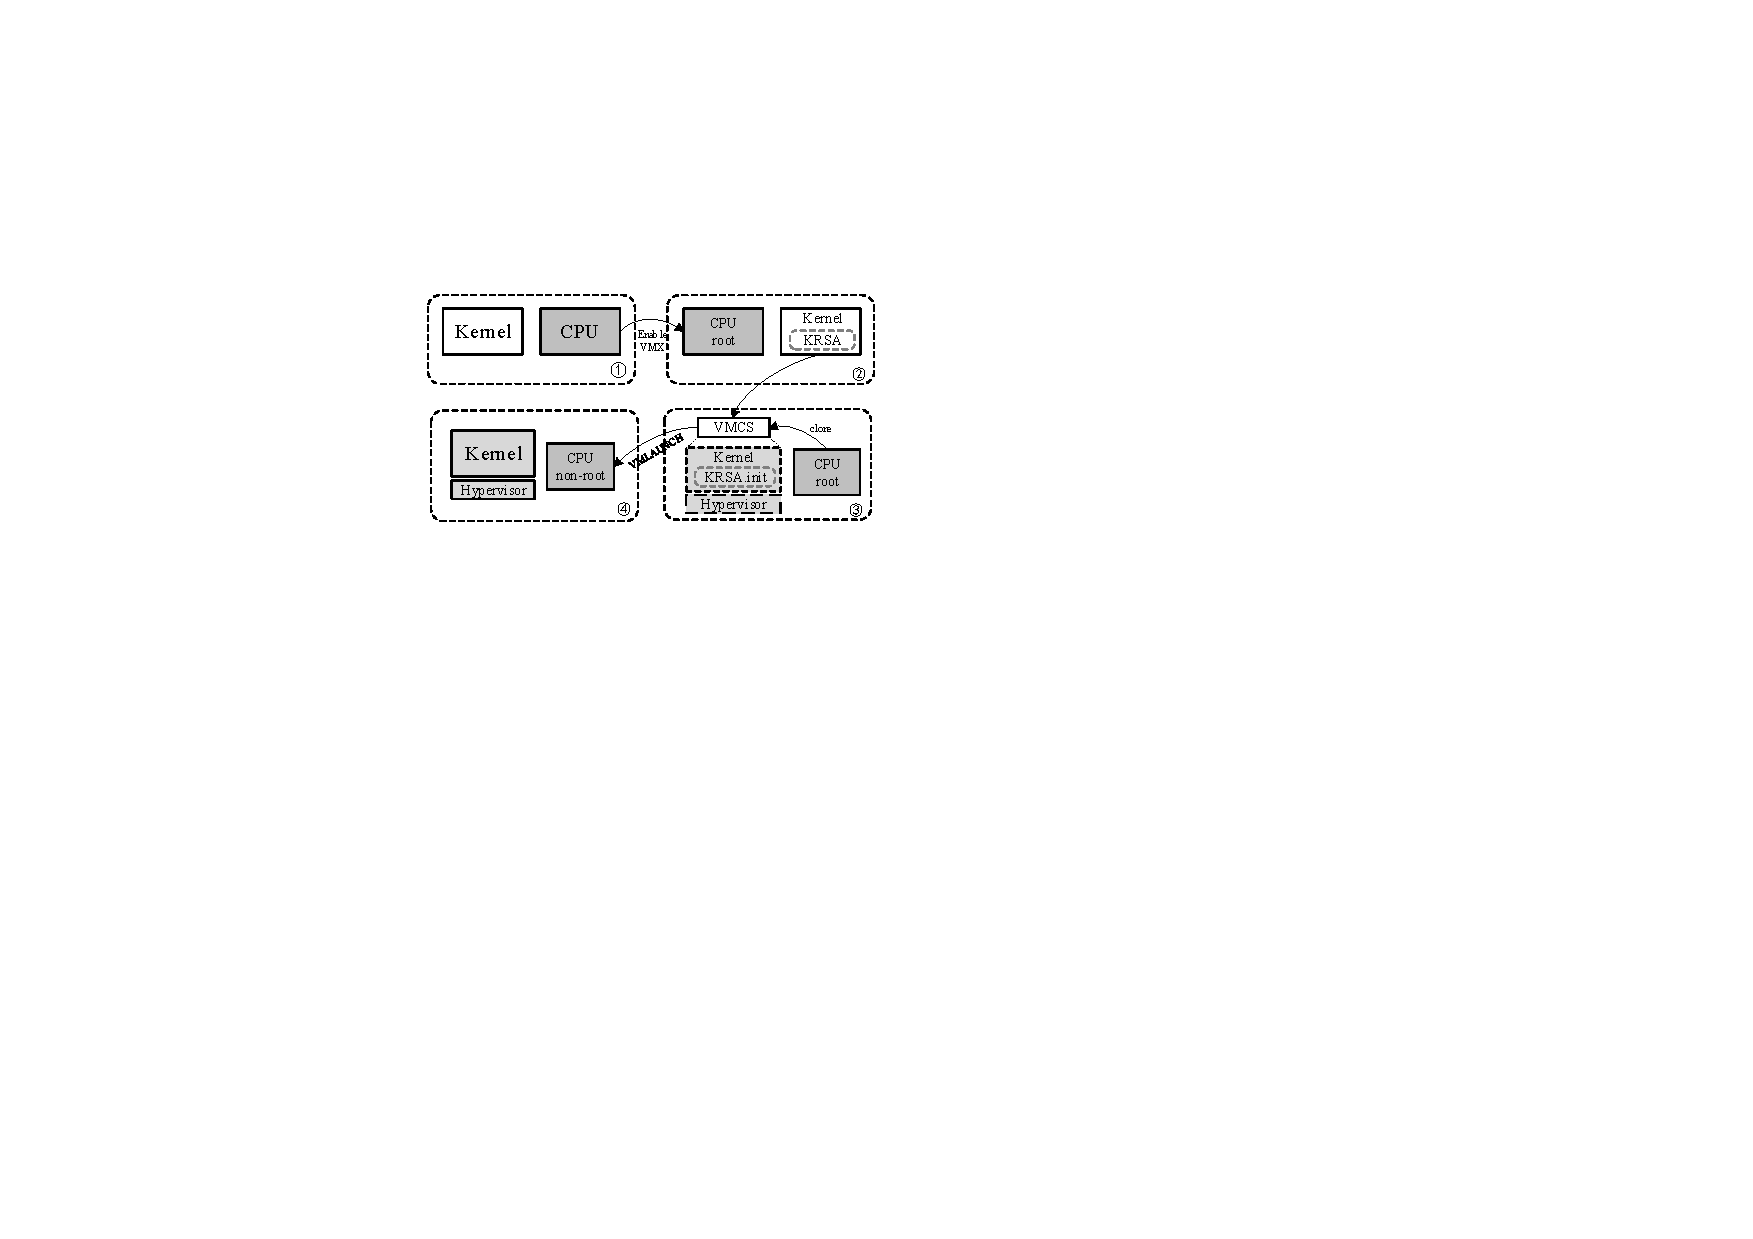
\includegraphics[width=7.5cm,height=4cm]{pic/trusted_boot.pdf}
%     \caption{Trusted Boot}
%     \setlength{\abovecaptionskip}{0pt}
%     \setlength{\belowcaptionskip}{0pt}
%     \label{pic_boot}
% \end{figure}
Firstly, The Trusted Boot component in Object Locating Engine would check if the hardware supports virtualization technology. If so, this component enables the hardware-assisted virtualization technology. At the same time, this component requests memory from the protected kernel to store KRSA relevant code and data and build a new memory mapping for them in proper memory address space after all memory regions have been allocated. When all the work mentioned above is complete, KRSA will enable VMX. Secondly, similar to the general virtualization startup process, Trusted Boot component initializes and set the VMCS region. Thirdly, VMLAUNCH would be called to launch the virtual processor, the protected kernel would run in the non-root mode. Lastly, Object Locating Engine would load other engines into memory and enable them. Finally, KRSA is trusted to be loaded into the execution environment. 


\section{Evaluation} \label{sec:eva}

\subsection{Security Analysis} \label{sec:seceva}
Our main goal is to prevent attacks that subverting kernel code, selected kernel data structures and efficient kernel page tables at runtime. For this, we choose several representative attacks to examine kernel security with KRSA. Table \ref{table:attacks} shows the attacks we use. 
% KRSA focuses on key kernel objects which mainly consist of kernel code and kernel structures. In order to measure the security of KRSA, we choose several representative attacks shown in Table \ref{table:attacks} to
% attack a system protected by KRSA.
% In this paper, we provide a systematical protection on various kernel objects including kernel code and kernel data structures. So that, as long as the developer pre-defines what data structures should be protected and what actions should be set to protect them, KRSA can provide a solid security enhancement. We choose the following attacks showed in Table \ref{table:attacks} as examples to measure the security of KRSA, because the attack targets pose extreme importance to kernel security and protected by KRSA.

\begin{scriptsize}
\begin{table}[h!]
  \centering
  \caption{Attack Cases}
  \begin{tabular}{c|c}
    \hline
    \textbf{Attack Name    } & \textbf{Attack Behavior} \\
    \hline
      sk2rc2  & Sys\_call\_table[\_NR\_oldolduname] \\
    \hdashline[.4pt/1pt]
      eNYeLKM 1.2 & kernel code modification \\
    \hdashline[.4pt/1pt]
      Adore-ng-2.6  & proc fs file operations table \\
    \hdashline[.4pt/1pt]
      SucKIT-2 & Interrupt descriptor table \\
    \hdashline[.4pt/1pt]
      POSTER & Master Kernel Page Table \\
    \hline
    \end{tabular}
  \label{table:attacks}
\end{table}
\end{scriptsize}

% By analyzing the behavior of these attacks, we find that the adversary can subvert the OS kernel in two ways: by modifying kernel data or by modifying kernel code. KRSA builds solid security enhancement on both ways to achieve systematically protection.
% By analyzing the behavior of these attacks, KRSA enhances the protected kernel from two aspects: maintain invariant of kernel code and protect kernel data.

% 这部分的写法是,首先写攻击者直接修改对应的物理内存中的内容,从而攻击内核。然后写double remap两种攻击,这两种攻击都是针对页表的攻击,从而危害代码和数据。
% 最后写lkm的问题。这样写,将代码和数据合并到一起写。


The most obvious way to subvert the kernel is to use various bugs to overwrite the program code or data in memory. The adversary usually makes a pointer invalid at first, and then dereferences the pointer, thereby triggering the error. \verb|NYeLKM| is one of these rootkits that exploit the kernel code through modifying the memory regions. \verb|SucKIT-2| and \verb|sk2rc2| are the rootkits that subvert kernel data, these rootkits modify the physical memory region that contains critical kernel data structures illegally. As a result, KRSA removes the write permission of all memory regions that contain kernel code or critical kernel data structures. KRSA clears the write permission of the EPT entries that manage these physical memory regions too. EPTs can only be modified by the KRSA's tiny hypervisor with a higher-level privilege than the kernel and the rootkit, thus, once the physical memory regions are registered through HandleRules, KRSA can achieve strong integrity reinforcement. 

Some rootkits, such as \verb|POSTER|, subvert the kernel by subverting corresponding page table entries. These rootkits redirect the pointer that points to critical kernel data to a fake one. They can also modify the page table entry to conduct re-mapping attack or double mapping attack. KRSA deprives the kernel with the capability of modifying the corresponding page table entries, so any write operation to relevant page table entries would be trapped into the hypervisor and handled by Object Protection Engine according to HandleRules.

\verb|Adore-ng-2.6| is another rootkit instance. This rootkit allows the adversary to subvert the kernel with an illegal LKM. LKM Protection Engine conducts integrity measurement to guarantee that all loaded LKMs are authorized by KRSA.

Some rootkits leverage virtual dynamic shared objects to executing userspace code with kernel privilege. KRSA employs protection mechanism such as ASLR, DEP/NX, SMEP to guard the integrity of kernel code.




% At first, for kernel code, with an elaborate on attacks, adversary tampers the kernel code by using the following three methods. The first kind of attack such as \verb|NYeLKM|, Because the protected kernel can not access to EPT which is maintained by the hypervisor with a higher privilege, on the one hand, write to the memory region that contains kernel code would always be captured and rejected by Object Protection Engine. On the other hand, page table entries who are involved in mapping kernel code

% Firstly, kernel data can be subverted using the following two method. The first kind of attack such as \verb|POSTER|, the adversary can subvert the kernel by using a forged fake kernel data. KRSA deprives the kernel with the capability of modifying the corresponding page table entries, so any write operation to relevant page table entries would be trapped into the hypervisor and handled by Object Protection Engine according to HandleRules. The second kind of attack such as \verb|SucKIT-2| and \verb|sk2rc2| subverts the physical memory region that containing protected kernel data. Because the protected kernel can not access to EPT which is maintained by the hypervisor with a higher privilege, write to this memory region would always be captured and rejected by Object Protection Engine.

% Secondly, for kernel code, with an elaborate on attacks, adversary tampers the kernel code by using the following three methods. The first kind of attack such as \verb|NYeLKM|, the same with what the attack does in data attack, conduct double mapping or re-mapping attack to subvert the kernel code in memory, thus both of these two aspects are reinforced by KRSA with the similar protection method. \verb|Adore-ng-2.6| is an attack instance for the second kind of attack, adversary subverts the kernel with an illegal LKM. LKM Protection Engine conducts integrity measurement to guarantee the LKM loaded into the kernel is authorized by KRSA. For the last kind of attack to kernel code, the attacker can use virtual dynamic shared objects to executing userspace code with kernel privilege. KRSA employs protection mechanism such as ASLR, DEP/NX, SMEP to guard kernel code.


% Firstly, we can prevent attacker from modifying the key data from two aspects. For the first aspect, the attacker can forge a fake data structure, then subvert the kernel to use the fake one, this kind of attack doesn't modify the real data but subvert the kernel successfully. One attack instance is POSTER. So KRSA deprives the kernel with the capability modifying the protected page table entries. Thus any operation to write these page table entries is authorized by KRSA, any attempt to write relevant protected kernel page tables will be trapped into the tiny hypervisor and disposed according to HandleRules.  For the second aspect, the attacker can tamper the kernel data structures on physical address directly, or the attacker can use double mapping to the protected kernel data structures. For this kind of attack such as SucKIT-2 and sk2rc2, KRSA let Object Protection Engine monitor the physical pages containing protected data Structures. Therefore the security of selected kernel data structures will be guaranteed by KRSA perfectly.

% Secondly, we guarantee that any code in kernel space is authorized by KRSA. After an elaborate analysis on these attacks on kernel code, we find that the attacker can tamper the kernel code using the following three methods. For the first kind of attack method, the attacker can modify the kernel code directly the same with the attacker dose in data attack. NYeLKM is a attack instance for this kind of attack. KRSA adopts the same protection method with data protection, mapping relationship and guest physical content are protected by Object Protection Engine. For the second kind of attack which conduct attack as Adore-ng-2.6 does, the attacker inserts a vicious LKM into kernel space. KRSA provides two hypercall to ensure that only authorized LKM can be loaded into kernel space. Integrity Measurement Engine would firstly calculate the kernel module, if the result is not satisfied with the result of the official kernel module, KRSA would forbid this kernel module to be loaded into the kernel. For the last kind of attack to kernel code, the attacker can use virtual dynamic shared objects to executing userspace code with kernel privilege. KRSA employs protection mechanism such as ASLR, DEP/NX, SMEP to guard kernel code.


% Please add the following required packages to your document preamble:
% \usepackage{multirow}
\begin{table*}[htbp]
\centering
\caption{Performance Comparisons Using LmBench}
\resizebox{\textwidth}{15mm}{
\label{table:lmbench}
\begin{tabular}{|c|c|c|c|c|c|c|c|c|}
\hline
    \multirow{2}{*}{\textbf{Index}} & \multicolumn{3}{c|}{\textbf{Context Switch}} & \multicolumn{5}{c|}{\textbf{System Call}}         \\ \cline{2-9} 
                                & 2p/16k      & 8p/16k    & 16p/16k   & null call   & fork proc   & sh proc     & open close & stat     \\ \hline
Native                          & 0.713       & 1.096     & 1.266     & 0.293       & 93.2        & 2163.33     & 1.080      & 0.733    \\
KRSA                           & 0.965       & 4.470     & 4.670     & 0.295       & 110         & 2430.5      & 1.135      & 0.735    \\ \hline
\hline
    \multirow{2}{*}{\textbf{Index}} & \multicolumn{8}{c|}{\textbf{Communication Bandwidths}}                                            \\ \cline{2-9} 
                                & pipe        & AF Unix   & TCP       & File Reread & Mmap Reread & Bcopy(libc) & Mem write  & Mem read \\ \hline
Native                          & 6159.666    & 6575      & 4679      & 6802.7      & 12.7        & 7626.166    & 7540.667   & 12       \\
KRSA                           & 6 5672.5    & 5909      & 4205.5    & 6733.85     & 12.5        & 7682.4      & 7519.5     & 11       \\
\hline
\end{tabular}
}
\end{table*}




\subsection{Performance Evaluation} \label{sec:perfeva}
% In order to test the performance of KRSA, we deploy KRSA on a Levono desktop computer with an Intel I5-4950T CPU and 8GB RAM.
% The architecture is implemented on ArchLinux with kernel 4.2.5. For a given terminal scenario, SELinux is widely used which bases on Linux Security Modules (LSM), in this scenario, after the elaborate analysis using Call Graph,
% We choose to protect the following kernel data structures.
% \textit{security\_hook\_heads} is chunked into section \verb|.krsa.data|, \textit{ia32\_sys\_call\_table}, \textit{idt\_table}, \textit{debug\_idt\_table}, \textit{trace\_idt\_table} are chunked into section \verb|.krsa.rodata|, and KRSA adopts HandleRules that have formulated before to protect these kernel objects.
% KRSA aims at this security scenario as the target and analyses key kernel data structures. KRSA chooses to protect the LSM, at this scenario, \textit{security\_hook\_heads}, \textit{security\_hook\_list} are chunked into \textit{Optional Protected Group}. \textit{sys\_call\_table}, \textit{ia32\_sys\_call\_table}, \textit{idt\_table}, \textit{debug\_idt\_table},\textit{trace\_idt\_table} are chunked into \textit{Basic Protected Group}. In this scenario, we just formulate HandleRules to forbid any write operation to object no matter they belong to \textit{Basic Protected Group} or \textit{Optional Protected Group}. Under the target environment, all performance tests are shown as following:

We measured the performance overhead incurred by KRSA based on LMBench and SPEC CPU2006. All measurements are taken on an Intel I5-4950T CPU with 8GB RAM. 
We choose to protect the following kernel data structures. 
\textit{security\_hook\_heads} is assigned into section \verb|.krsa.data|, \textit{ia32\_sys\_call\_table}, \textit{idt\_table}, \textit{debug\_idt\_table}, \textit{trace\_idt\_table} are assigned into section \verb|.krsa.rodata|, and KRSA developed corresponding HandleRules and recompiled the kernel using the method mention above. 

% \paragraph{Micro Benchmark Evaluation}
We use a subset of the context switch, system call, and communication bandwidths microbenchmarks from LMBench to study our overheads. Table ref{table:lmbench} shows the result of our experiments.
For overheads of communication bandwidths, there is no significant difference between KRSA and the native kernel. 
The \textit{null call}, \textit{stat} and \textit{open close} show the overhead of system call without frequent process operation is acceptable. 
The overhead of \textit{fork proc} and \textit{sh proc} are quite high, since KRSA interrupts \textit{load\_cr3} operation, KRSA costs a large time to deal with virtualization environment context switch. CR3 cache queue in CPU can mitigate this kind of performance overhead, but, there are only four CR3 cache candidates in hardware. 


% Table \ref{table:lmbench} shows the result of the performance overhead introduced by KRSA compared with the native OS. As shown in the table, because of KRSA mainly focuses on kernel objects loaded into the memory, little performance overhead on Communication Bandwidths is introduced. Besides, System Call without frequent process operation, for example \textit{null call}, \textit{stat} and \textit{open close}, performs acceptable which only introduces at most 5\% performance overhead.
% Because of hardware limitation (the experimental CPU only has four cores, four CR3 cache queues), as the number of processes increases, the performance overhead of Context Switch becomes more and more significant, when the perform overhead seems to be acceptable in 2p/16K item. some System Call, such as \textit{fork proc} and \textit{sh proc} performs poorly due to the same reason with Context Switch. However in terminal environment, unlike server environment, ordinary work does not involve with frequent process operations.
% We use lmbench to examine the performance overhead introduced by KRSA compared with the native OS. The result is shown in Table \ref{table:lmbench}. Memory operations achieve almost as the same performance as the native OS. Also, KRSA poses almost no influence on I/O operations and networking communication. For these I/O related test items such as \textit{open close} , KRSA poses at most 5\% performance overhead, and for these network related test items such as \textit{slct tcp} , KRSA poses at most 1\% performance overhead.
% This is because I/O and network are not the targets should be protected according to our threat model, as the result, hypervisor in KRSA does not virtualize these two aspects. However, operations such \textit{context switch},\textit{fork proc} and \textit{sh proc} seem to gain performance loss. In detail, KRSA also gain an acceptable overhead in 2p/16K text item, when the process come into 8 or 16, the performance seems to be large. The reason is that our CPU has only four cores and four CR3 Cache Queue, the hardware can not cope with tasks beyond its hardware core numbers. The reason why items such as \textit{fork proc} and \textit{sh proc} perform poorly with about 14\% overhead on average is as the same as the reason in \textit{context switch}, because all these tests involve with context switch. However in desktop environment, little work requires frequent context switch.
% From the results, we can conclude that KRSA has little performance overhead in most of test items, and KRSA can be applied into the desktop environment.


% \paragraph{Application Performance Evaluation}

Figure \ref{spec} summarizes the performance impact of KRSA compared to a non-modified kernel. 
The result of \textit{bzip2}, \textit{perlbench}, \textit{hmmer} and \textit{gcc} show that the deviations among KRSA and the non-modified kernel are small (\textless2\%).
The result of \textit{mcf} shows that KRSA has significant delay by large memory allocation and deallocation. The result implies that when large memory allocation happened in the kernel, KRSA costs a large time consumption to load pages and update page table. 
\textit{astar} and \textit{omenttpp} incur the overhead because of frequent context switch.

% vmOS has a significant delay caused by the kernel module memalloc intervening in the MMU. It implies that when missing page happened in vmos, it costs a large time consumption to load pages and update page table.
%
% The performance is represented as the average and maximum overhead using SPEC CPU 2006 in Figure \ref{spec}.
% We use SPEC CPU 2006 to test the application performance overhead introduced by KRSA compared with the native OS. The result is shown in Figure \ref{spec}.
% Most of items (\textit{bzip2}, \textit{perlbench}, \textit{hmmer} and \textit{gcc}) that can be used on a daily use gain about 2\% overhead on average. KRSA introduces acceptable performance overhead for most of ordinary works in desktop environment. Some applications require large memory allocation such as \textit{mcf} encounter relatively large performance losses wiht 17\%, this is because page table entries are modified frequently which would cause KRSA check the operation frequently. \textit{astar} and \textit{omenttpp} encounter performance loss because of frequent context switch. However for a ordinary use in terminal environment, these applications are not routinely used on a daily basis, so the performance introduced by KRSA is acceptable.

\begin{figure}
    \centering
    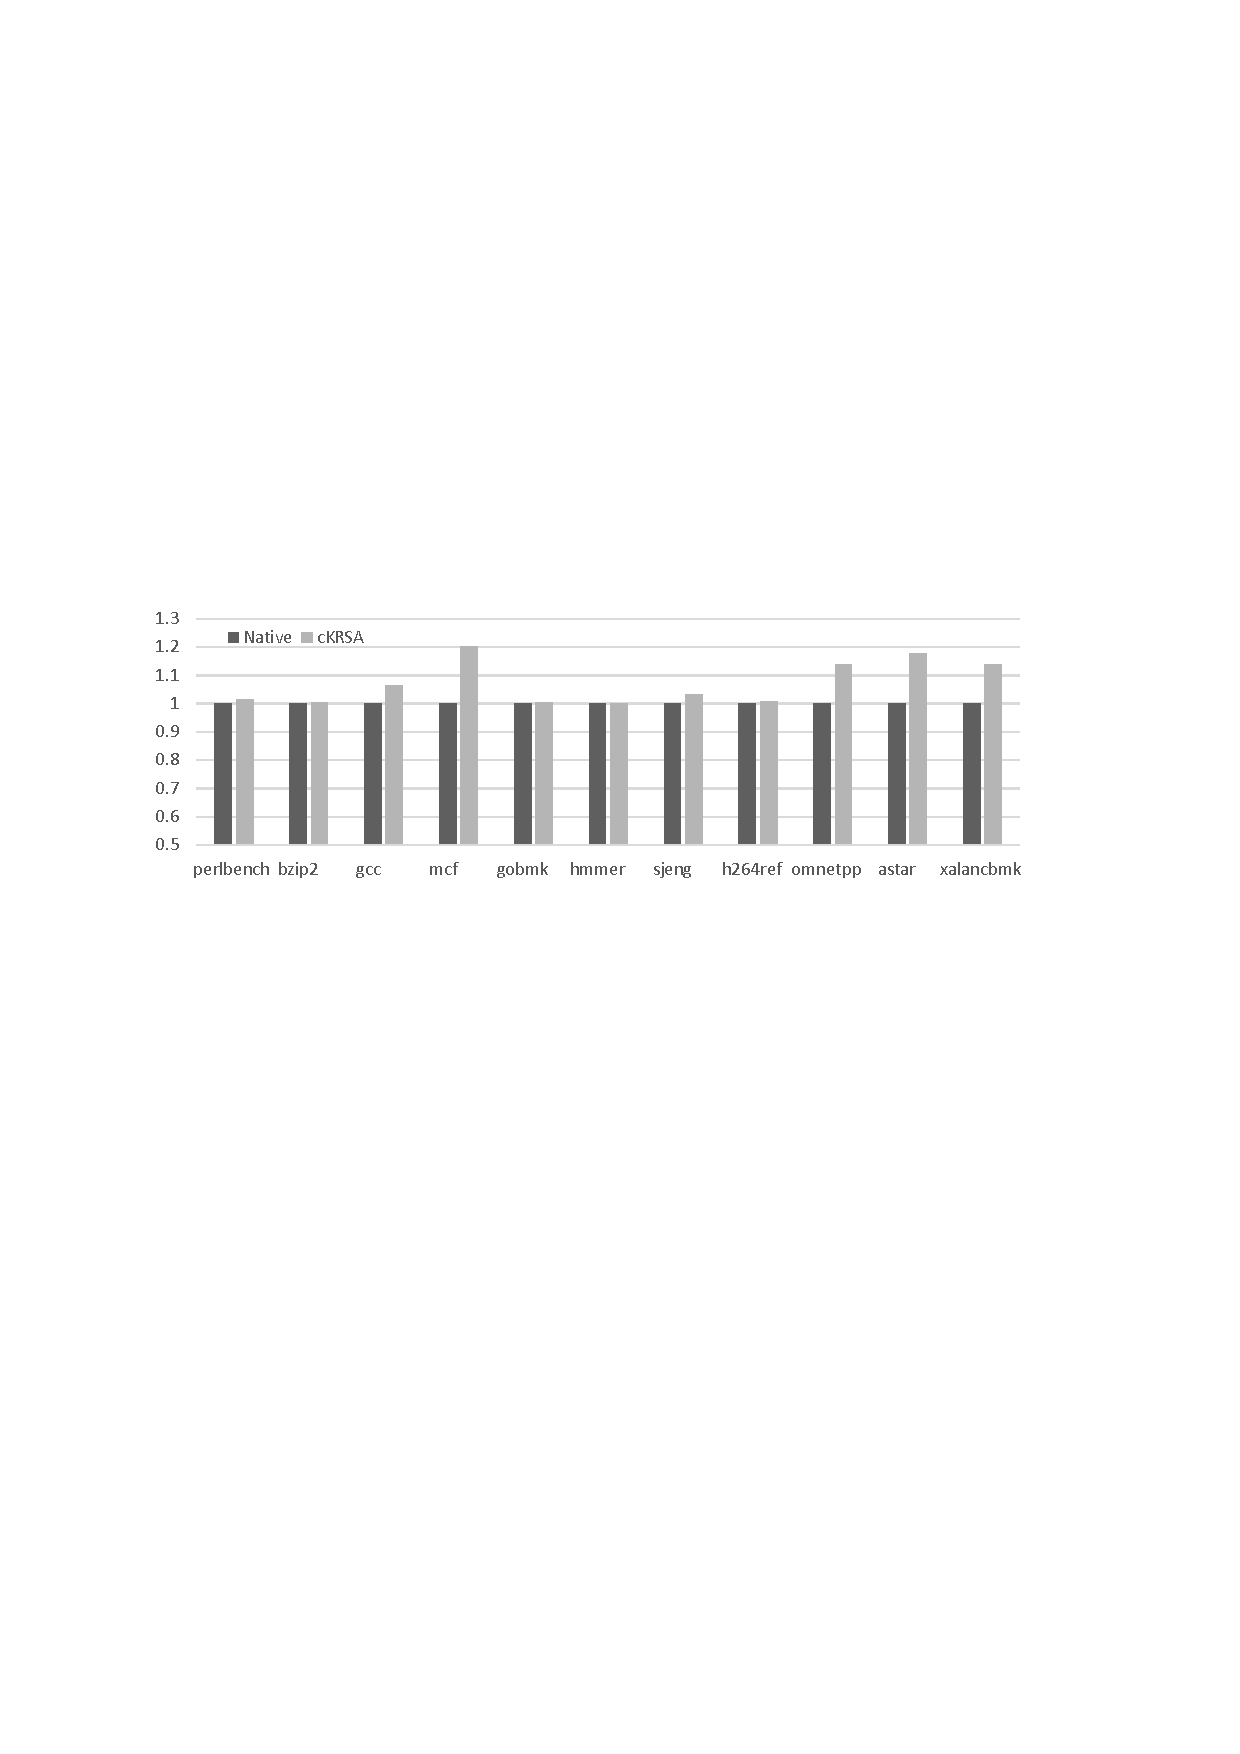
\includegraphics[scale=0.5]{pic/spec_1.pdf}
    \caption{Performance tests using SPECCPU 2006}
    \label{spec}
\end{figure}



% \section{Limitation}
% % KRSA is a systematical protection architecture for a customizable scenario. We have shown its conception through experiments with a prototype. However the current prototype of KRSA is not at its full maturity. We describe the limitations of the current prototype in this section.
% KRSA is a customizable kernel runtime security architecture to provide systematical kernel protection, covering kernel code and kernel data, in a given terminal scenario. Kernel code is protected from being modified, added and deleted by the methods provided by KRSA. KRSA also prevents adversary from executing code in userspace with kernel privilege. Kernel data however faces more complex protection situations, in general, data can be divided into two types: statically-allocated and dynamically-allocated kernel data. If the kernel data is declared and initialized before the kernel running, such as \textit{sys\_call\_table}, KRSA does provides a series of methods to protect the integrity of the data. However, dynamically-allocated data usually allocated in stack or heap, it would cost much if the detect them during runtime, and direct protection to them with hypervisor also incurs huge performance loss.
% Some complex and subtle availability attacks such as ROP, JOP, DOP mainly leverage those dynamically-allocated kernel data to compromise the kernel, KRSA could only raise the threshold for such attacks through the protection of critical statically-allocated kernel data who is also important for control flow integrity. We will continue to protect against attacks that aim at dynamically-allocated data and control flow on the basis of existing work in the further work.

\section{Related Work}
Regardless of how the attack changes, it must eventually be settled into the kernel code and kernel data, thus various protection schemes are proposed to address these attacks. 
% Some works(OSck\cite{ensosck}, Stider GhostBuster\cite{strider}, VMwatcher\cite{outbox}, HyperTap\cite{invariant}) propose hypervisor-based solution to detect rootkit that compromise the kernel.
Some hardware-assisted solutions, such as Copilot\cite{coplilot}, Vigilare\cite{vigilare}, Ki-Mon\cite{ki-mon}, introduce additional hardware to monitor memory or take snapshots of the memory to detect if the protected kernel is compromised. In contrast, KRSA relies on virtualization technology which has been widely deployed in commercial processors.
% KRSA is for the prevention of kernel rootkits execution in the first place by protecting the predefined data structures and kernel text from being manipulated by them.
% SecVisor\cite{secvisor}, Patagonix\cite{hyperbina} propose some security enhancements, such as PXN/SMEP, implemented by using software methods have been replaced by the hardware mechanism applied in KRSA. In order to protect kernel,
% Lares\cite{secarch},
Nested kernel\cite{nest15} and PT-Rand\cite{ptrand} provide kernel security by protecting the kernel page table. KRSA approves of the importance of page table and achieves page table protection without modifying page table related kernel code. Furthermore, KRSA provides more granular page table protection based on page table entries.
% pay attention to kernel page table, which is shared with KRSA, but KRSA achieves our protection requirements and better performance by only protecting just a part of page table entries.

% SecVisor\cite{secvisor}, Patagonix\cite{hyperbina} propose some security enhancements, such as PXN/SMEP, implemented by using software methods have been replaced by the hardware mechanism applied in KRSA. In order to protect kernel,
% Lares\cite{secarch}, Nested kernel\cite{nest15} and PT-Rand\cite{ptrand} pay attention to kernel page table, which is shared with KRSA, but KRSA achieves our protection requirements and better performance by only protecting just a part of page table entries.

Some solutions inspire us to implement KRSA, SecVisor \cite{secvisor} use the tiny hypervisor to protect kernel code, however, it does not support protection to kernel self-modifying code and data structures. 
NICKLE\cite{vmmshadow} uses memory shadowing and instruction emulation to protect kernel code, while KRSA protects kernel data as well and achieves better performance with the help of hardware. HookSafe\cite{hooksafe} mainly focuses on protecting kernel hooks and control flow integrity, while KRSA emphasizes on systematical protection to kernel code, critical kernel data structures, and effective page tables. 
% protection to the selected kernel
% objects involved with security threaten in a given scenario.
% pays attention to the integrity of kernel code and critical kernel data to protect the security functions and modules in a given scenario.
Nested kernel\cite{nest15} implements the same protection purposes, but requires the user to be fully aware of the kernel and has the ability to modify kernel, whereas KRSA only requires users to be able to identify the objects they want to protect and locate them in source code. In the process of implementing KRSA, we also draw on a series of protection schemes for our tiny hypervisor, including formal verification\cite{sel413}, 
% ,sel4} ,
security enhancements%\cite{memsafe}
\cite{hypersentry,hyperSafe}, and size reduction \cite{break,seccloud}.
% ,nova,seccloud}.



\section{Conclusion}

Exploits against the kernel are highly dangerous as they allow the attacker to execute malicious code with operating system privileges. In this paper, we have presented the design, implementation, and evaluation of KRSA, a tiny-hypervisor-based runtime kernel protection architecture that can protect kernel code, critical kernel data structures, and efficient page tables. We have implemented a tiny hypervisor with small code size to avoid a large number of vulnerabilities in commodity hypervisors. We have put forward HandleRule to define critical kernel data structures. 
We have taken kernel self-modifying code into consideration when we enforced kernel code with integrity policy. We have classified page table entries into five categories which provide accurate protection to kernel code and kernel data structures. The evaluation shows that KRSA meets the balance between performance and security. 

% Linux is now widely deployed in a variety of terminals. In different scenarios, Linux requires multifarious security features that require a systematical protection architecture which can be customized for the given scenario. For this reason, in this paper, we propose a customizable kernel runtime security architecture, called KRSA to meet the balance between performance and security.
% By analyzing specific scenario using Call Graph, KRSA can find out all kernel data that is critical to enable the security features in the given scenario.
% With the help of hardware-assisted virtualization technology, KRSA can provide systematical protection by reinforcing the integrity and legitimate access permission for kernel code and critical kernel data. Furthermore, because of the wide adoption of hardware virtualization technology on commodity hardware, KRSA can also be smoothly applied to other commodity hardware platforms.

% KRSA mainly focuses on the protection to of kernel code and critical data in its integrity and legitimate access permissions in the terminal scenario. With the help of Virtualization Technology, kernel code and selected kernel data will not be compromised by a series of attacks such as direct modification, double mapping, at runtime.

% The security of operating system kernels is an open problem, and recent hardware virtualization technologies enable the protection of the kernel. In this paper, we propose a customizable kernel runtime security architecture, called KRSA, focusing on the integrity and access permissions of the kernel code and key kernel data structures specified for various security scenarios, monitored by a tiny hypervisor with commodity hardware for Intel X86 processors, so then it systematically ensures the kernel runtime security involving with code protection, data protection and control-flow protection. In practice use, KRSA can provide the protection for some user-space and kernel-space excellent security mechanisms such as Selinux, seccomp, IMA, DEP, ASLR and so on, to enhance the security of the whole operating  system together.  Otherwise, from the research on different types of kernel attacks, the definition of key kernel data structure in various security scenarios will be more sufficient and reasonable, the security effectiveness of KRSA will be better to face more complex attacks.






% 原本的设计内容
% 参考的文章的内容摘抄
\iffalse

% Another issue is about how to track dynamic data for both kernel and extensions. To address this, HUKO inserts a trusted driver (labeled as a trusted extension) into the oprating system to notify the hypervisor about the allocation and reclamation of the kernel memory. The driver is also aware of the owner subject of each page and reports updates to the hypervisor during runtime.
the hypervisor would trap all events that modify this page regardless of the current protection state. 
When the kernel memoty access control policy permits a mediated write operation, Sentry must reproduce the effects of the operation in a guest operating system`s memory. This functionality resides in Sentry because the guest operating system cannot execute the write opration itself due to the write protection bit set on the faulted page. We implemented an instruction emulator inside the hypervisor to perform the emulation of memory writes. 
Because only the hypervisor can write to the memory pages of protected kernel hooks ,we will transfer the control from the guest kernel to the hypervisor to commit the update and then switch back to the guest kernel. 


For page table
the second step is to enforce that all memory pages used for page tables are mapped as read-only in logical mapping. This is done as follows. (1)XXXX

To handle the formal case, XXX To protect this table ,we map it inaccessible under normal context. Similarly, to prevent attackers from traversing page tables through arbitrary memory read, page tables for XXX are also mapped as inaccessible under normal context. 

We choose page tables, rather than other MMU-based protection schemes, such as segmentation, because page tables are supported by a large number of CPU architectures. 
using page tables requires Secvisor to protect the page tables from being modified by any entity but Secvisor and its TCB.
There are two ways to achieve this. One, 
The guest kernel maintains its own page tables to translate virtual addresses to guest physical addresses.  This two step translation from virtual to system physical addrss is illustrated in Figure. 

We walk the page table using the address translation engine to verify that the virtual to physical address mapping that correspond to the LKM's code region has been deleted. 

Accesses to physical memory pages are subjected to permission checks in both NPT and guest kernel page tables. 

It also requires modifications to the kernel's page table handling code which XXX.%在hypervisor中实现内核的功能
Certain Linux kernel text and data structures, including page tables, are located at a specific invariant location in virtual memory and are mapped linearly, allowing for the retrieval of page tables and thus the locations of data structures that would otherwise be difficult to determine. Once the locations are known, it then reconstructs the guest OS semantics based on kernel data structure knowledge that was also manually extracted. 
KRSA operates on the EPT, which is managed by the hypervisor. 
% An attacker who is in control of guest page tables can launch memory remapping attacks. KRSA thwarts this attack by keeping both virtual and physical address of protected pages in the hypervisor. since any update to guest page table will be synced to EPT, KRSA verifies wheter any protected virtual addresses have been remapped. If so, KRSA protects additionally the new physical pages.
Any update to the guest page table in the guest kernel is trapped and progagated to the SPT by the hypervisor, In other words, the hardware performs the address translation solely with the SPT. 
Enabling and disabling WXN bit does not affect the protection because page tables can override
The second phase works by modifying the shadow page table code of Xen.%这段可以为初始化的时候,第二阶段做什么
Hooksafe utilizes the shadow page table realized in the hypervisor for a running guest VM and sets proper protections for memory pages of the protected contents. %实现部分使用
It implies that when missing page happened in vmOS, it costs a large time comsumption to load pages and update page table. %评估部分使用


As previously mentioned, the MonitoringRules that operate in KI-Mon are built with the KI-Mon API. The KI-Mon API, as shown in Figure 4, includes high-level software stacks and low-level drivers for the hardware platform, to enable convenient and rapid development of kernel integrity monitoring rules. KI-Mon API is developed so that writing new MonitoringRules, based on our detection methodology, become convenient. It is even possible to create entirely new algorithms. 

XX is the main component in the software platform, enabling the event-triggered monitoring mechanmism.
It interfaces with HandleRules, 
Critical regions and their whitelists are stored in VTMU upon the registration of MonitoringRules.A MonitoringRule is also required to have predetermined actions such as an HAW-Event Handler and an Integrity Verifier, to be executed when HAW-Events occur in the critical regions. These actions are fetched and executed by KI-Veri.

The key idea is to monitor the value of selected kernel data structures during runtime, and hypothesize invariants that are satisfied by these data structures. 

KRAS specify what code regions of the kernel are allowed to write what data objects within kernel memory. 

these character device has been abused by attacker as a mechanism to inject malious code or tamper with kernel data structures.
for instance attacks that tamper with kernel data structure by directly injecting values into kernel memory (through vulnerabilities or by abusing /dev/kmem)

once the locations are known, it then reconstructs the guest OS semantics based on kernel data structure knowledge that was also manually extracted. 
legerages the debugging sysbols to mutate the fields of the kernel data structure out-of-VM with duplicate-value-directed semantic field fuzzing to estimate the severity of kernel data structure manipulation attacks. 
which uses gcc to derive kernel data structure invariants. 
leverages kernel source code to distinguish different heap data structures and then constructs the kernel heap graph to facilitate in understanding kernel malware behavior. 
extracts the memory management data structures from kernel source code. 
recompiles kernel source code with special padding such that a binary rewriter can be applied and the control flow transfer can be observed and enforced at the hypervisor layer. 
modifies the kernel source code to partition the kernel data structure layout such that it can detect and prevent malicious modifications to critical kernel data structures that are protected by the hypervisor. 
it analyze source code to determine the forms and locations of kernel data structures of interest. 
MAS statically analyze kernel source code to build benign kernel data structure graph. 
KI-mon is example of systems that detect kernel data modification. 
use memory access restrictions to protect kernel data. 
quite a few security accproaches utilize the knowledge of kernel data structures to achieve find-grained auditing and intrusion detection.
memory regions for kernel code, kernel data and extensions are usually page aligned, which facilitates the labeling procedure in KRSA. 

for page table 
the labeling component must be able to track objects within two categories of mix pages: pages containing both kernel code and kernel data. 
considing a mixed page that has mixed label of both kernel data and extension code, the hypervisor would trap all events that modify this page regardless the current protection state. Then KRSA examines the physical address to see if it is in the range of extension text area and finally determines the object identity. 
for static objects such as kernel code, static kernel data, and trusted entry points, KRSA tracks them by leveraging the kernel symbol table. 

the second category of exceptions consists of OS kernel data of which the kernel XXXX

the follow-up efforts extend to examine the violation of kernel data integrity or state-based kernel control flow integrity. 

KRAS specify what code regions of the kernel are allowed to write what data objects within kernel memory. 

malware that attempts to hide itself or process by manipulating kernel data will trigger an access violation in KRSA. 


% 用作相关工作中
Copilot is a kernel integrity monitor that uses a PCI add-in card to access memory instead of relying on kernel to accoplish that. it uses MD5 hashes of kernel text, LKM's text and the contents of the system call table as its detection strategy. The same authors of Copilot address its limitation of no being applicable to dynamic kernel data structures with an architecture that dectects kernl violation by comparing the kernel state with a specification of a correct state done by an expert. 

% 这段用于安全分析和lkm防护。
the module's init function is usually the place where rootkits presenting themselves as LKM tamper with kernel structures, such as the system call table. the adore rootkit, for instance, replaces the entry of 15 system calls with its own malicious function. 
we cannot offer protection against attacks that do not need to write into kernel space to succeed. 

% The zone watermarks for each zone are stored in a global data structure called `zone\_table`. the location of this table can be found by referring to the System.map file.the only form of kernel data tampering performed by rootkits pertains to hiding the malicious objects. such object hiding deceives the user into believing that he has a clean system.

% Control transfer from user code into the kernel: system calls (traps) and user program events (faults)

% Control transfer from the kernel to user code: signals APCs syscall return.

% once the system is booted, every entry to the kernel occurs as a result of an event. event handlers are kernel-defined and execute in kernel mode.

% the common approach followed by all mainstream OSes to ensure kernel code integrity is through kernel access control mechanisms and kernel-enforced restrictions on module loading.

which is accomplished by the introduction of hooks in certion points of kernel code

% malware exploiting vulnerabilities in kernel code that allow direct injection of network bytes into kerel memory.


Kernel contains countless kernel objects (kernel code, control data, non-control data) during runtime, that makes kernel protection to be a tremendous work. However it does not mean that all of the kernel objects should be monitored and protected. Actually most of kernel objects, especially kernel data, pose no influence on kernel security. Meanwhile, security requirements are different in different security scenarios, thus the customized kernel would adopt different security features and solutions. Based on the facts mentioned above, only particular kernel objects should be selected and protected by KRSA. On the other hand, most attacks, such as code corruption attack, control-flow hijacking attack, data-only attack and information leak attack, primarily focuses on kernel code and kernel data that has been loaded into memory, so KRSA mainly chooses to protect the picked kernel objects who have been loaded into memory. 

%首先代码段是必须要保护起来的,为什么要保护代码???保护哪些代码???为什么保护全部的代码而非部分代码???
Kernel code is one of the kernel objects who must be protected with no doubt.
For kernel code, KRSA guarantees the integrity of all kernel features. KRSA guarantees that the functionality that is formed by the benign kernel code would be properly enabled and powered. KRSA also blocks the load and execution of unauthorized kernel code, such as shellcode or malicious LKM code imported by attacker. 

% 要保护的数据因为场景不同而不同,那么,如何界定在不同场景中需要保护的需要保护的数据?KRSA通过分析控制流图的方法得到所有关键的,不可绕过的关键的数据点。首先,针对特定的场景,其启用的安全模块或者安全功能是不同的,KRSA将在这个场景下,必须使用的模块或者功能一般已经被标记为一个基本块(BB),然后通过依赖关系分析,向上找到到系统调用或者中断向量表为止的所有的路径,记录下在这些路径中所使用的关键的数据结构点,构成一个集合。其次,对所有的集合取交集,则这些点就是使能当前安全方案或者功能的关键的,不可绕过的数据结构。这些数据结构就是我们要保护的关键数据结构。将在这个场景中,所有必须使用的关键的bb进行分析,取并集,就是针对这个给定的场景中,需要保护的所有的关键数据结构。
For kernel data, the data that needs to be protected varies depending on the scenario. In a given scenario, on the one hand, not all kernel data needs to be protected, on the other hand, for these kernel data to be protected, different kernel data needs different protection strategies. So the first problem that KRSA needs to address is to find the data that deserve to be protected, and what protection policies should be adopted. For a specific scenario, the user should first well know and figure out which kernel functions or modules should be protected. Then, KRSA uses the Call Graph (CG) and standard dependency analysis to analyze the kernel control flow to obtain the target data that needs to be protected, and this method is shared by most control flow integrity solutions \cite{cfisurvey}. 
% More details would be illustrated in Section \ref{section:aggre}.
% KRSA uses call graph (CG) to identify all key data structure. Firstly, KRSA gets the CG for the customized kernel in the given scenario. In CG, in general, the security module or function we focus on in this scenario is as an end point. Secondly, KRSA uses standard dependency analysis to recursively find each path that end of this end point. In our analysis, each path we get would end with \textit{sys\_call\_table} or \textit{idt\_table}, because KRSA just protect the customized kernel. Thirdly, KRSA formulates all data in the path into a set, and conducts intersection operation to all sets that end with a same end point. Fourthly, KRSA marks the data in all the collections from the third step as data to be protected, but different data need to be protected with different permissions, thus, KRSA uses different label to tag different kernel data. In our preliminary design, the type of labels is related to the type of permission required by the kernel object. Assuming that only RWX(read, write, execution) is considered for data kernel object, KRSA has designed two type of labels: Read-Only, Read-Write.
% 通过上述的X步骤得到的最后的数据集合就是KRSA要保护的数据,这些数据为所有控制流路径上不可绕过的点。一般而言,这些数据都是一些关键的branch数据。因此,保证对这些数据的合法访问,就可以保证在特定应用场景中,被保护的关键功能能被正确使能。
% In fact, the each kernel data obtained through the four step above is a point that cannot be bypassed on all control paths, and these data generally are key bracnch data. Therefore, The legitimate access to these data reinforced by KRSA can ensures that the security module or function protected in a particular scenario can be properly enabled.
At last, KRSA inserts labels to all protected kernel objects, and recompile the customized kernel with a new linker script. After this step, objects with same access permission would be allocated to the same page-aligned memory area during runtime.

Figure \ref{recompile} depicts how KRSA tags the protected kernel object and how the protected kernel objects are distributed in memory after using method provided by KRSA. 

\begin{figure}
    \centering
    % 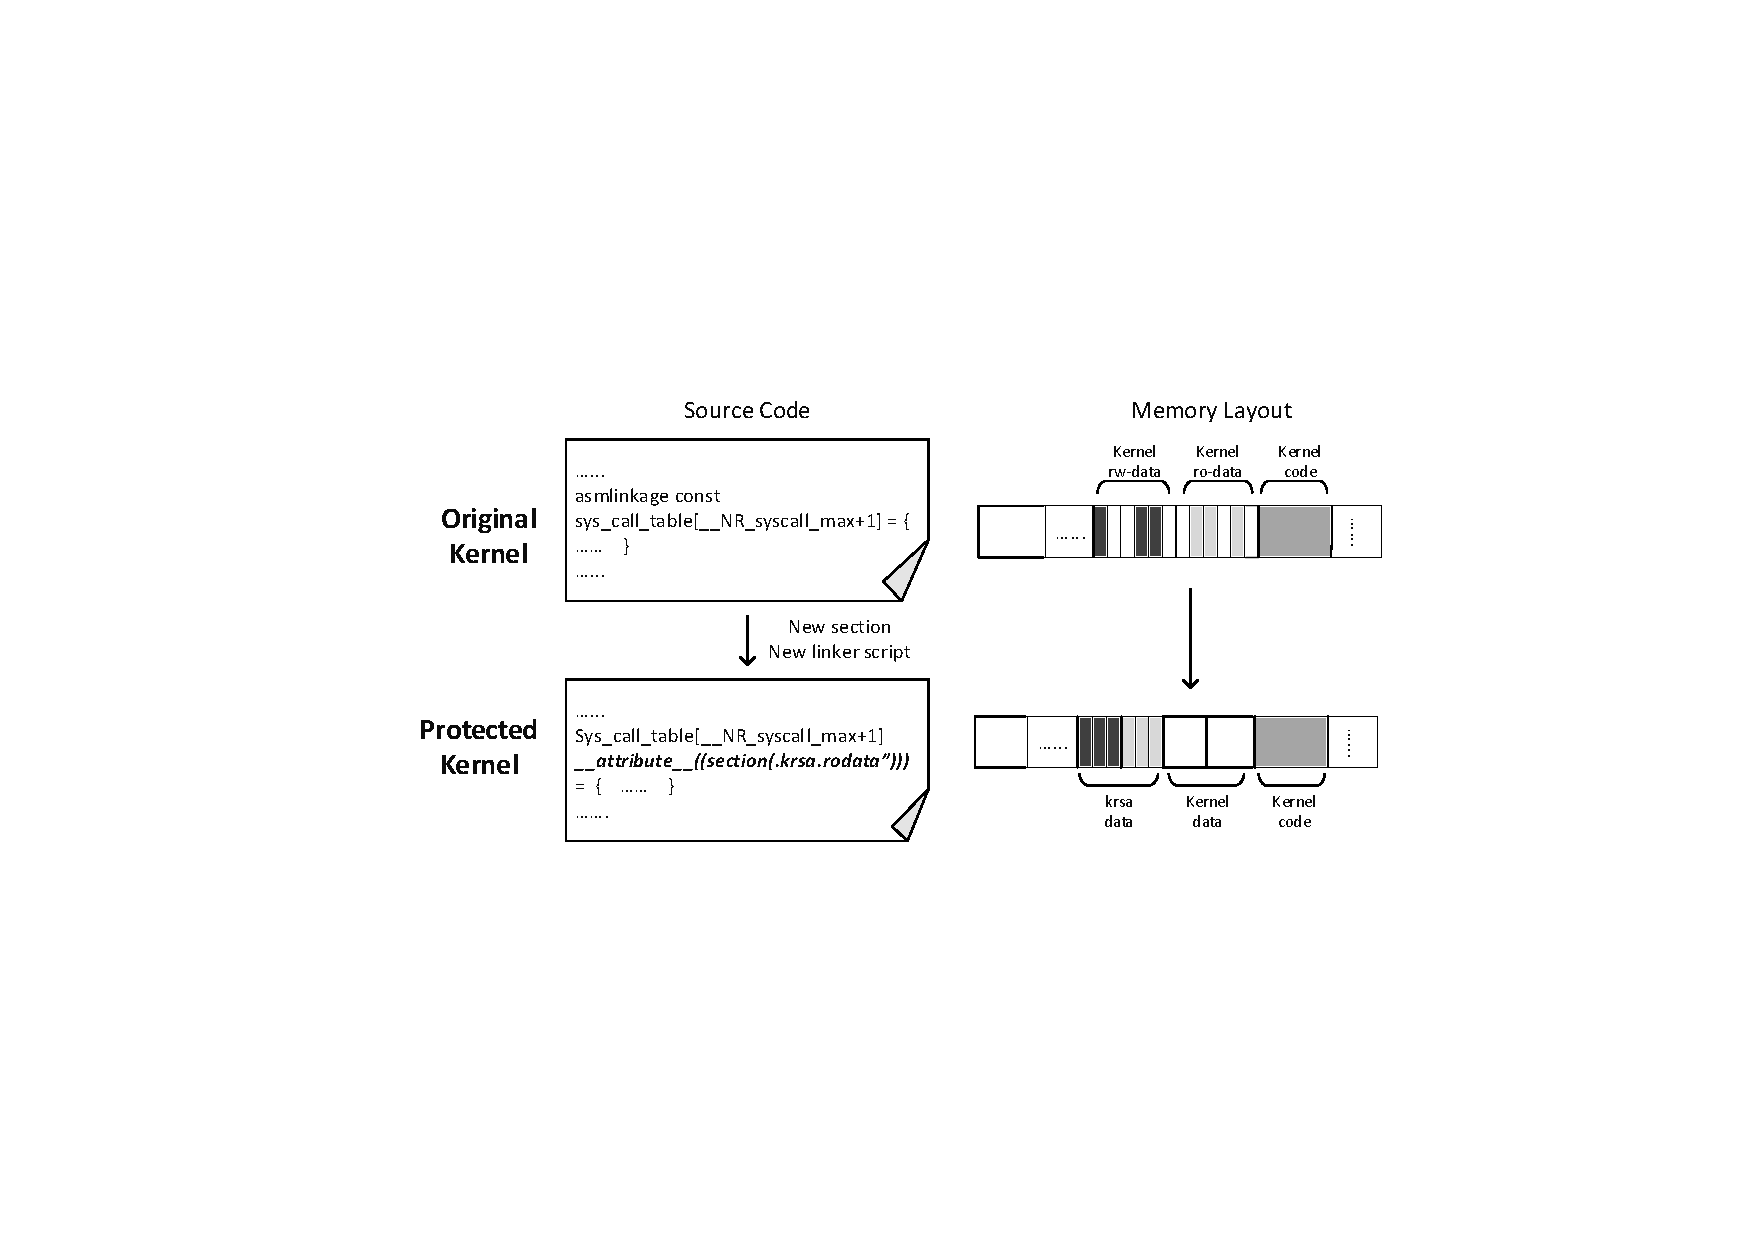
\includegraphics[width=1\textwidth,height=0.35\textwidth]{pic/data_aggregate.pdf}
    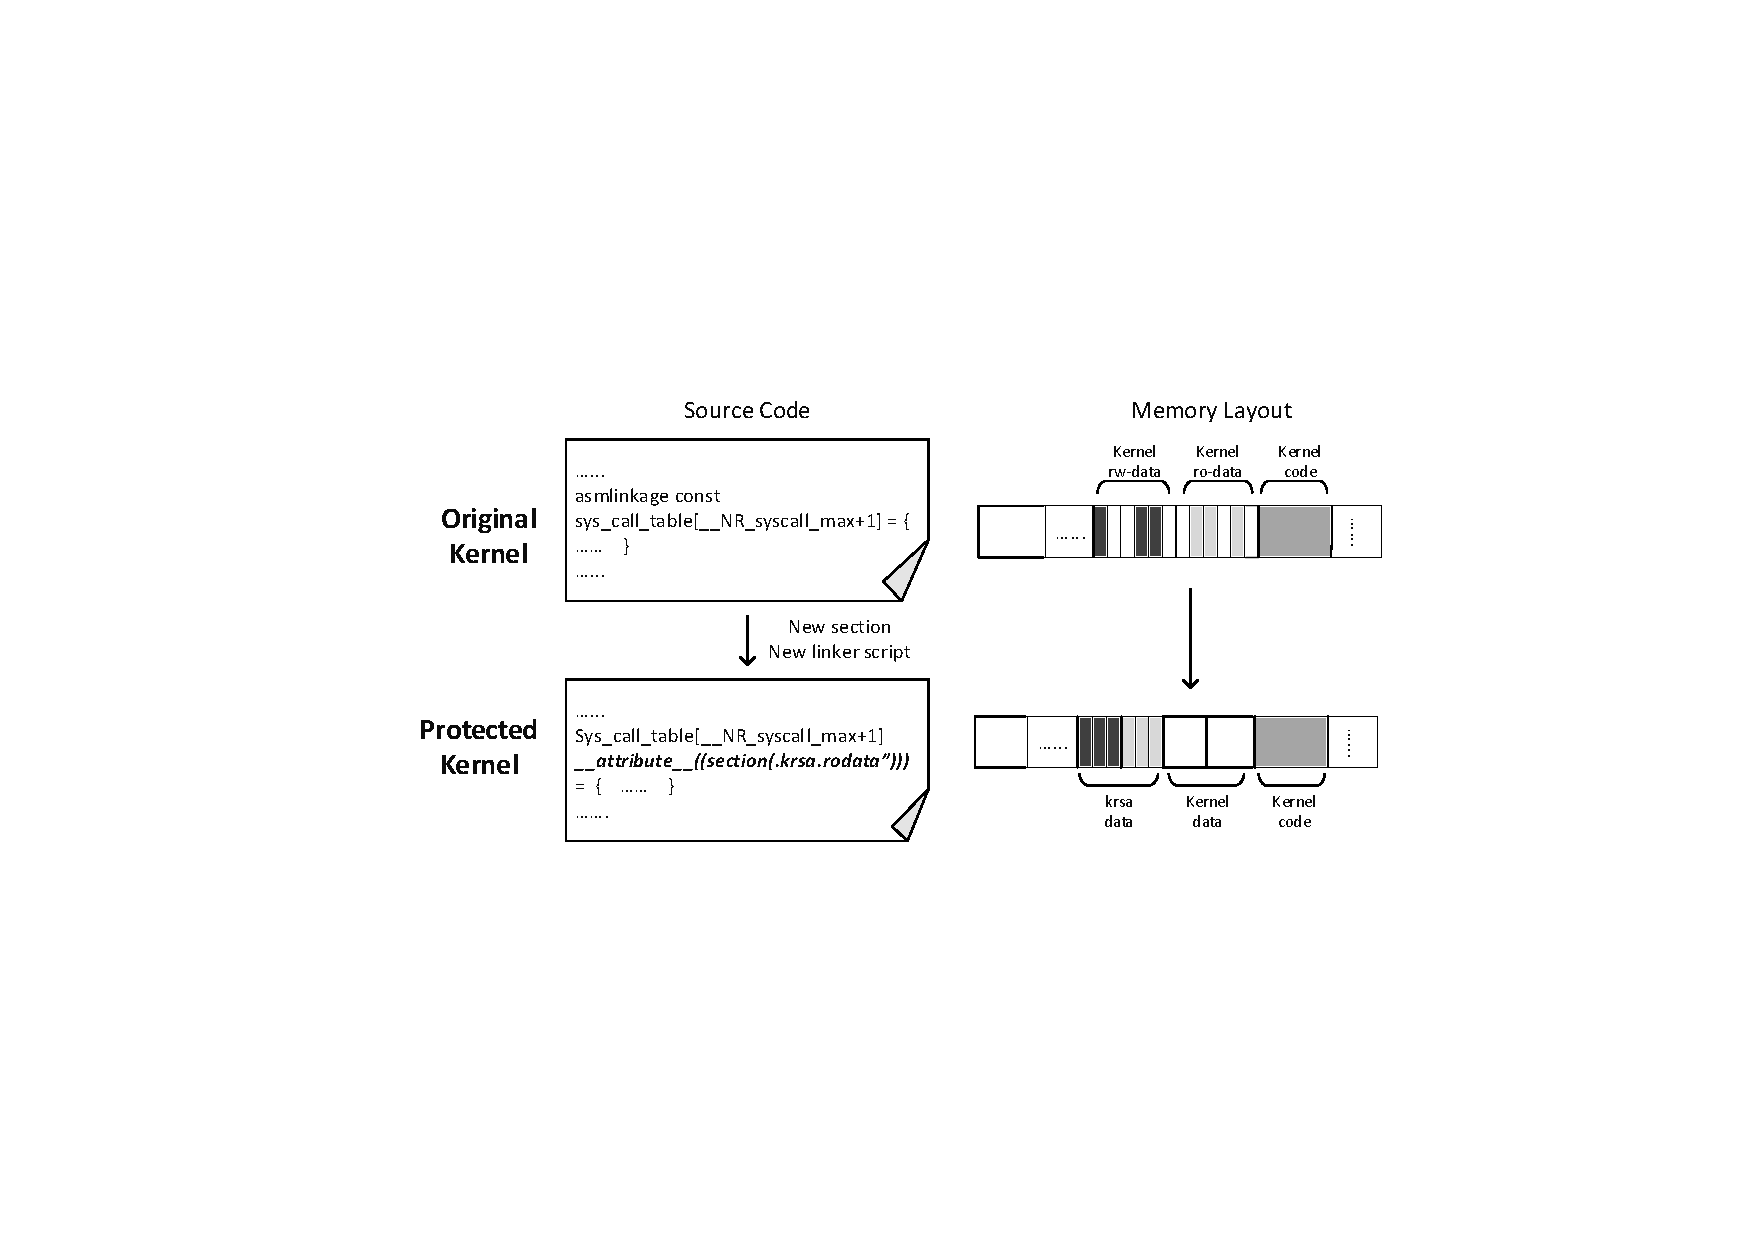
\includegraphics[scale=0.5]{pic/data_aggregate.pdf}
    \caption{Object Selection}
    \label{recompile}
\end{figure}


% \begin{figure}[htb]
% \begin{minipage}[b]{0.52\textwidth}
%   \centering
%   \begin{tabular}{lccc}
%       \hline\noalign{\smallskip}
%     \textbf{Object} & \textbf{Label } & \textbf{Flags} & \textbf{Example}\\
%     \hline
%       Code & No & RO & Kernel text \\
%     \hdashline[.4pt/1pt]
%       RO-data & Yes & RO & sys\_call\_table \\
%     \hdashline[.4pt/1pt]
%       RW-data & Yes & RW & security\_hook\_heads \\
%     \end{tabular}
%   \caption{Protected Kernel Objects}
%   \label{table:protect_object}
% \end{minipage}
% \begin{minipage}[b]{0.48\textwidth}
%     \centering
%     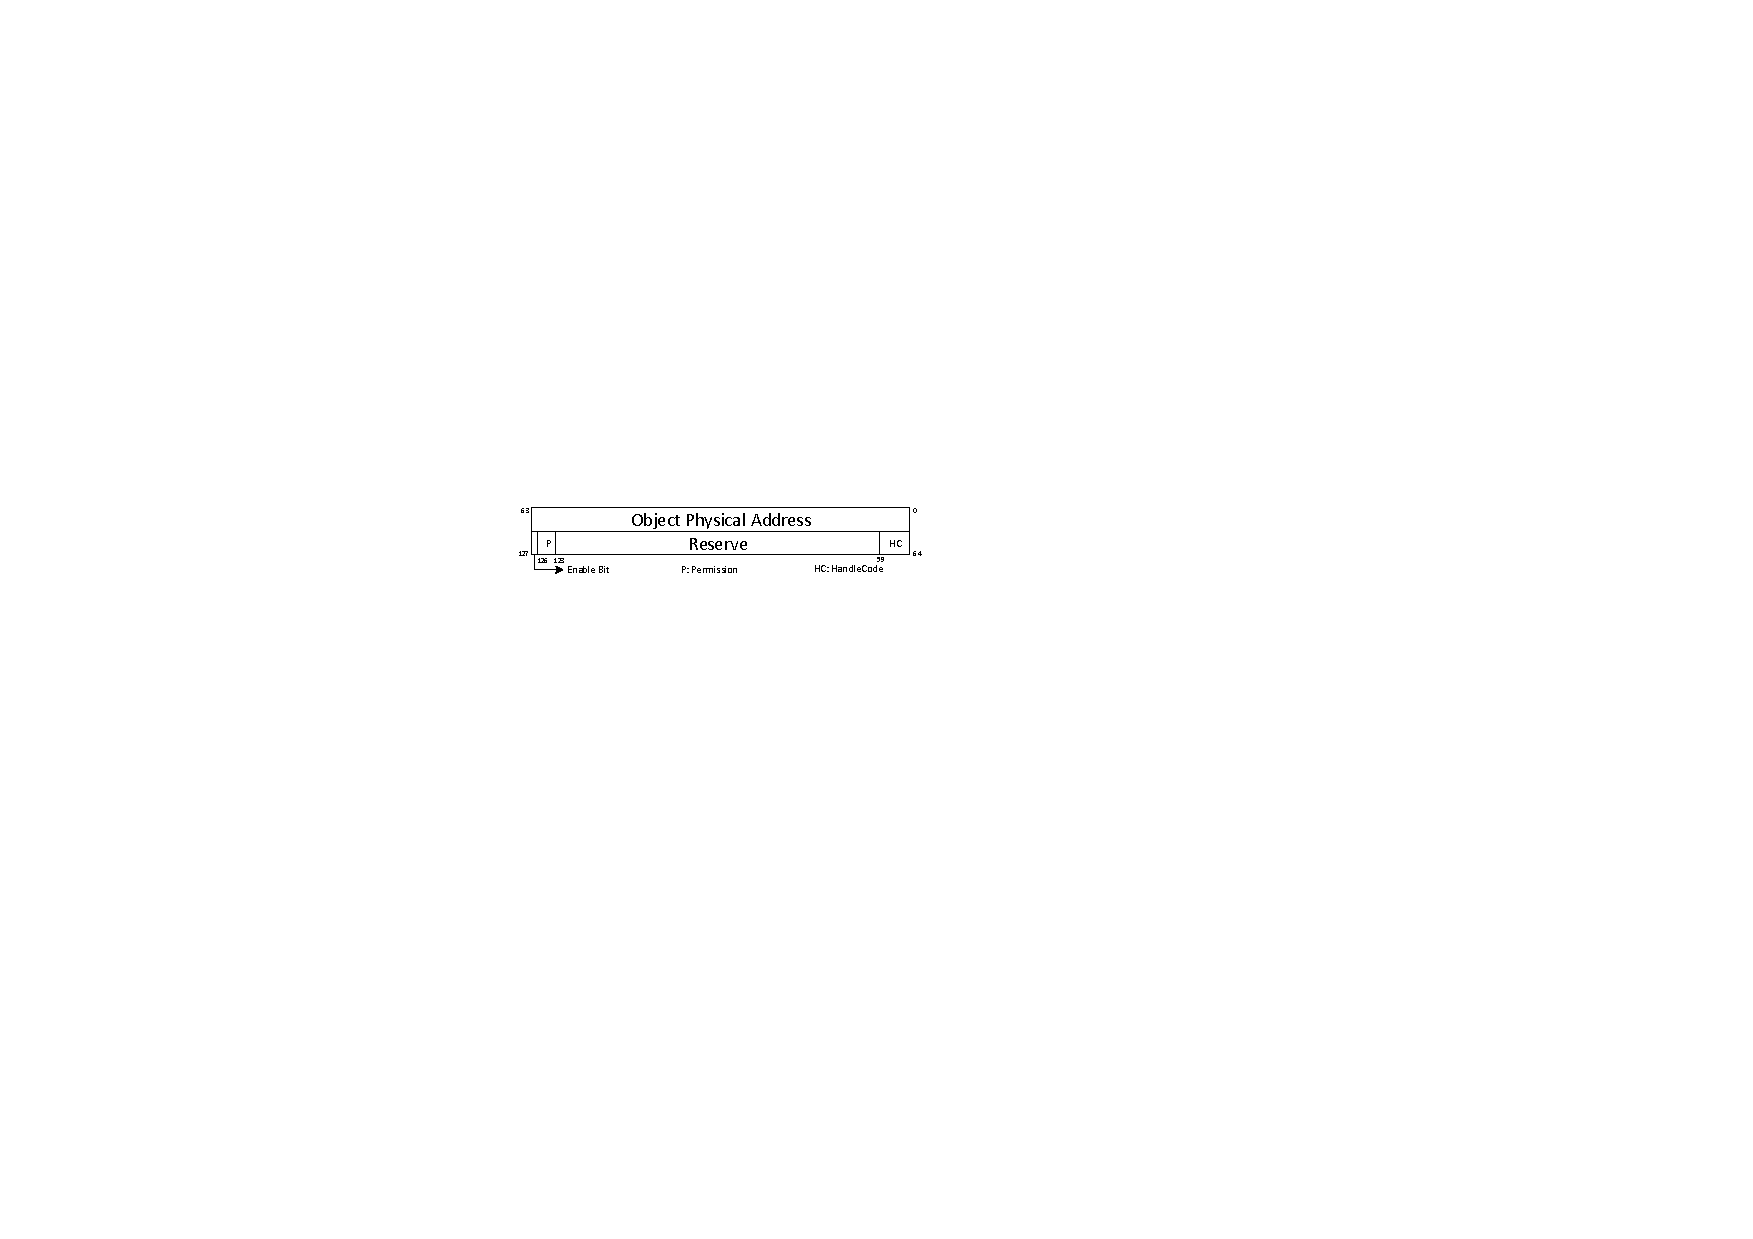
\includegraphics[scale=0.96]{pic/handlerules.pdf}
%     \caption{HandleRules}
%     \label{rulefigure}
% \end{minipage}
% \end{figure}



% \begin{scriptsize}
% \begin{table}[h!]
%   \centering
%   \caption{Protected Kernel Objects}
%   \begin{tabular}{|c|c|c|c|}
%     \hline
%     \textbf{Object} & \textbf{} & \textbf{Flags} & \textbf{Example}\\
%     \hline
%       Code & Direct & Read-Only & Kernel text \\
%     \hline
%       RO-data & Modified & Read-Only & sys\_call\_table \\
%     \hline
%       RW-data & Modified & Read-Write & security\_hook\_heads \\
%     \hline
%     \end{tabular}
%   \label{table:protect_object}
% \end{table}
% \end{scriptsize}
%


% 在不同的场景中,因为其安全功能需求不同,所以其保护的数据各不相同,但是不同场景的保护数据必然会存在一定的交集。KRSA通过对多个场景分析,找到了在每个场景中都需要被保护的数据,一般而言,这些数据要求的保护策略也是一样的,为了方便使用,KRSA已经对这些数据结构,例如系统调用表等,制定了保护策略。
In different scenarios, the protected data is different because of the different security requirement, but there is bound to be a Disjunction (AND) group between the protected data sets, and these data generally adopt the same protection policies. In order to facilitate the use of KRSA, KRSA locates all these data and develops default protection policies for them. For example, \textit{sys\_call\_table} usually should be marked to be read-only, thus KRSA reinforces this policy. 
% Figure \ref{table:protect_object} gives a summary on how KRSA protect kernel objects.



% through the analysis of multiple scenarios, and the protection policies to these data, in general, would remain to be the same. In order to facilitate the use of KRSA, KRSA has developed protection policies to these data, such as \textit{sys\_call\_table} and so on.

\subsection{Runtime Framework} \label{section:frame}

KRSA designs and employs three engines with higher privilege to protect kernel objects at runtime as depicted in Figure \ref{arch}. Each engine boils down to a set of units of work, and the HandleRules instructs all these three engines to achieve systematical protection for the kernel objects declared in Section \ref{section:scope}. 
% There are four important components in this framework: Object Locating Engine, Object Protection Engine, LKM Protection Engine and HandleRules.
% The three engine as depicted in the figure boils down to a set of units of work, HandleRules combines them to enable systematical protection.

\begin{figure}
    \centering
    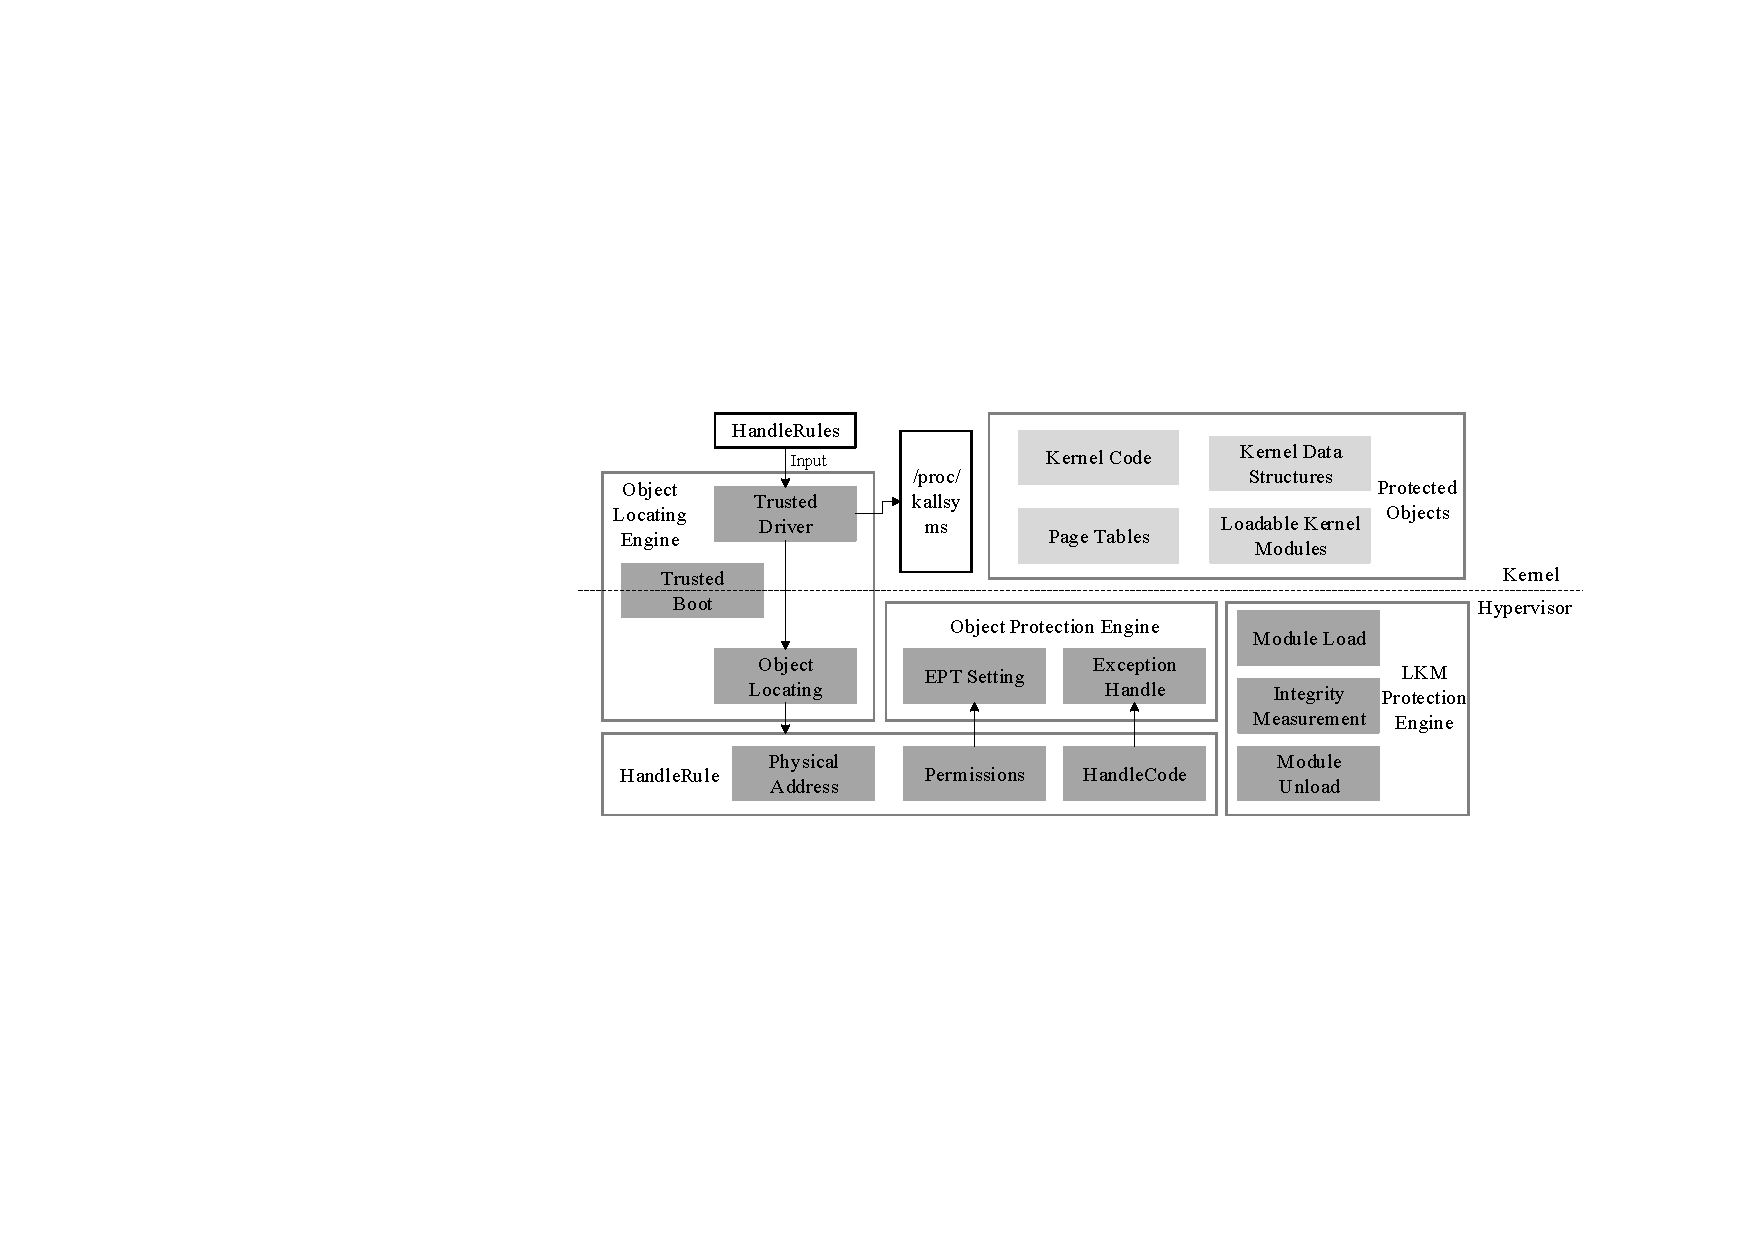
\includegraphics[scale=0.5]{pic/architecture.pdf}
    \caption{Runtime Framework}
    \label{arch}
\end{figure}

% \paragraph{Object Locating Engine}
\subsubsection{Object Locating Engine}
% Object Locating Engine, as an interface between the protected kernel and Object Protection Engine, is primarily responsible for three aspects of work.
Object Locating Engine is primarily responsible for trusted booting, locating the protected kernel objects at runtime and formulating corresponding HandleRules. 
Firstly, Object Locating Engine is the first loaded KRSA's module and is responsible for booting and initializing all remaining modules of KRSA. As the first loaded kernel module, KRSA needs a trusted switch from the protected kernel to these protection engine. Secondly, Object Locating Engine is responsible for traversing all protected objects labeled in Section \ref{section:scope} and forming HandleRules.
% which would be illustrated in Section \ref{section:handlerules}. HandleRules, one of the most important concepts used by KRSA, is used to instruct how Object Protection Engine works.
% Actually, this step accomplishes most of the work of Object Locating Engine as an interface.
At last, Object Locating Engine would interface with LKM Protection Engine and formulate corresponding HandleRules for the imported module. 
%Lastly, this Engine involves the management work of new generated protected kernel objects at runtime. This aspect of the work is primarily focus on the protection of new objects introduced at runtime. 
\subsubsection{Object Protection Engine}
Object Protection Engine is responsible for enabling all security guidance mechanisms according to HandleRules. In details, the main task for this engine is to accomplish the following four works. 
Firstly, Object Protection Engine is charge of monitoring and managing the memory of protected kernel. Actually, based on the current computer architecture, the CPU always fetches code and data from memory, 
% and general attacks, including ROP and side-channel attack, inevitably involve objects in memory. Thus
thus KRSA must be solely responsible for the memory of the protected kernel. Secondly, Object Protection Engine would set protection to these kernel objects that delivered through HandleRules. The process would be illustrated in Section \ref{section:workflow}. 
% In the system initialization phase, Object Protection Engine first reads the kernel objects that need to be protected and their protection requirements from the HandleRules, and then sets specific protection policies for kernel objects based on protection requirements.
Thirdly, when the security violation occurs, Object Protection Engine handles the security violation according to the context and HandleRules. 
%KRSA implements the protection of the customized kernel, allowing the user to define how to protect specific kernel data, each handler defined by user is assigned with a HandleCode before running. When the security violation occurs, KRSA will find the HandleCode according to the context, then boot into the corresponding handler.
Lastly, Object Protection Engine ensures the security of Object Locating Engine which works in the protected kernel.

\subsubsection{LKM Protection Engine}
LKM Protection Engine is introduced to handle loadable kernel module protection, three works are mainly handled by this engine. Firstly, Integrity measurement is performed on receiving the signal that the protected kernel is going to load a new loadable kernel module, this step would ensures that the newly introduced modules are authorized modules. Secondly, LKM Protection Engine would interface with Object Locating Engine after a LKM is loaded into memory. This engine delivers the information, such as where the module code is load to and where the specific data is, to Object Locating Engine. Loadable kernel module actually is loaded and executed with kernel privilege, so KRSA must take the newly introduced kernel module code and data into consideration, especially when user defines some objects to be protected in the newly introduced kernel module. 



\subsubsection{HandleRules}
HandleRules is a new conception proposed by KRSA to meet the security requirements in various scenarios. In detail, HandleRules is a structure that maintains the address of protected kernel objects and their security attributions. Figure \ref{rulefigure} depicts the structure of HandleRules.
% to facilitate user to designate the protected kernel objects, KRSA itself also need a structure to implement the corresponding protection. Figure \ref{rulefigure} depicts the structure of HandleRules.
% Each engine as depicted in the figure boils down to a set of units of work, HandleRules combines them to enable systematical protection.
% in different scenarios, the kernel object that need to be protected  varies depending on the scenario, KRSA need

% After inserting labels and recompiling the customized kernel source code using the method as described in section \ref{section:scope}, KRSA employs a hypervisor to protect all marked kernel objects. In this process, KRSA proposes a new conception: HandleRules. Because in different scenarios, the protected kernel object varies depending on the scenario, KRSA need a structure to facilitate user to designate the protected kernel objects, KRSA itself also need a structure to implement the corresponding protection. Figure \ref{rulefigure} depicts the structure of HandleRules.

\begin{figure}
    \centering
    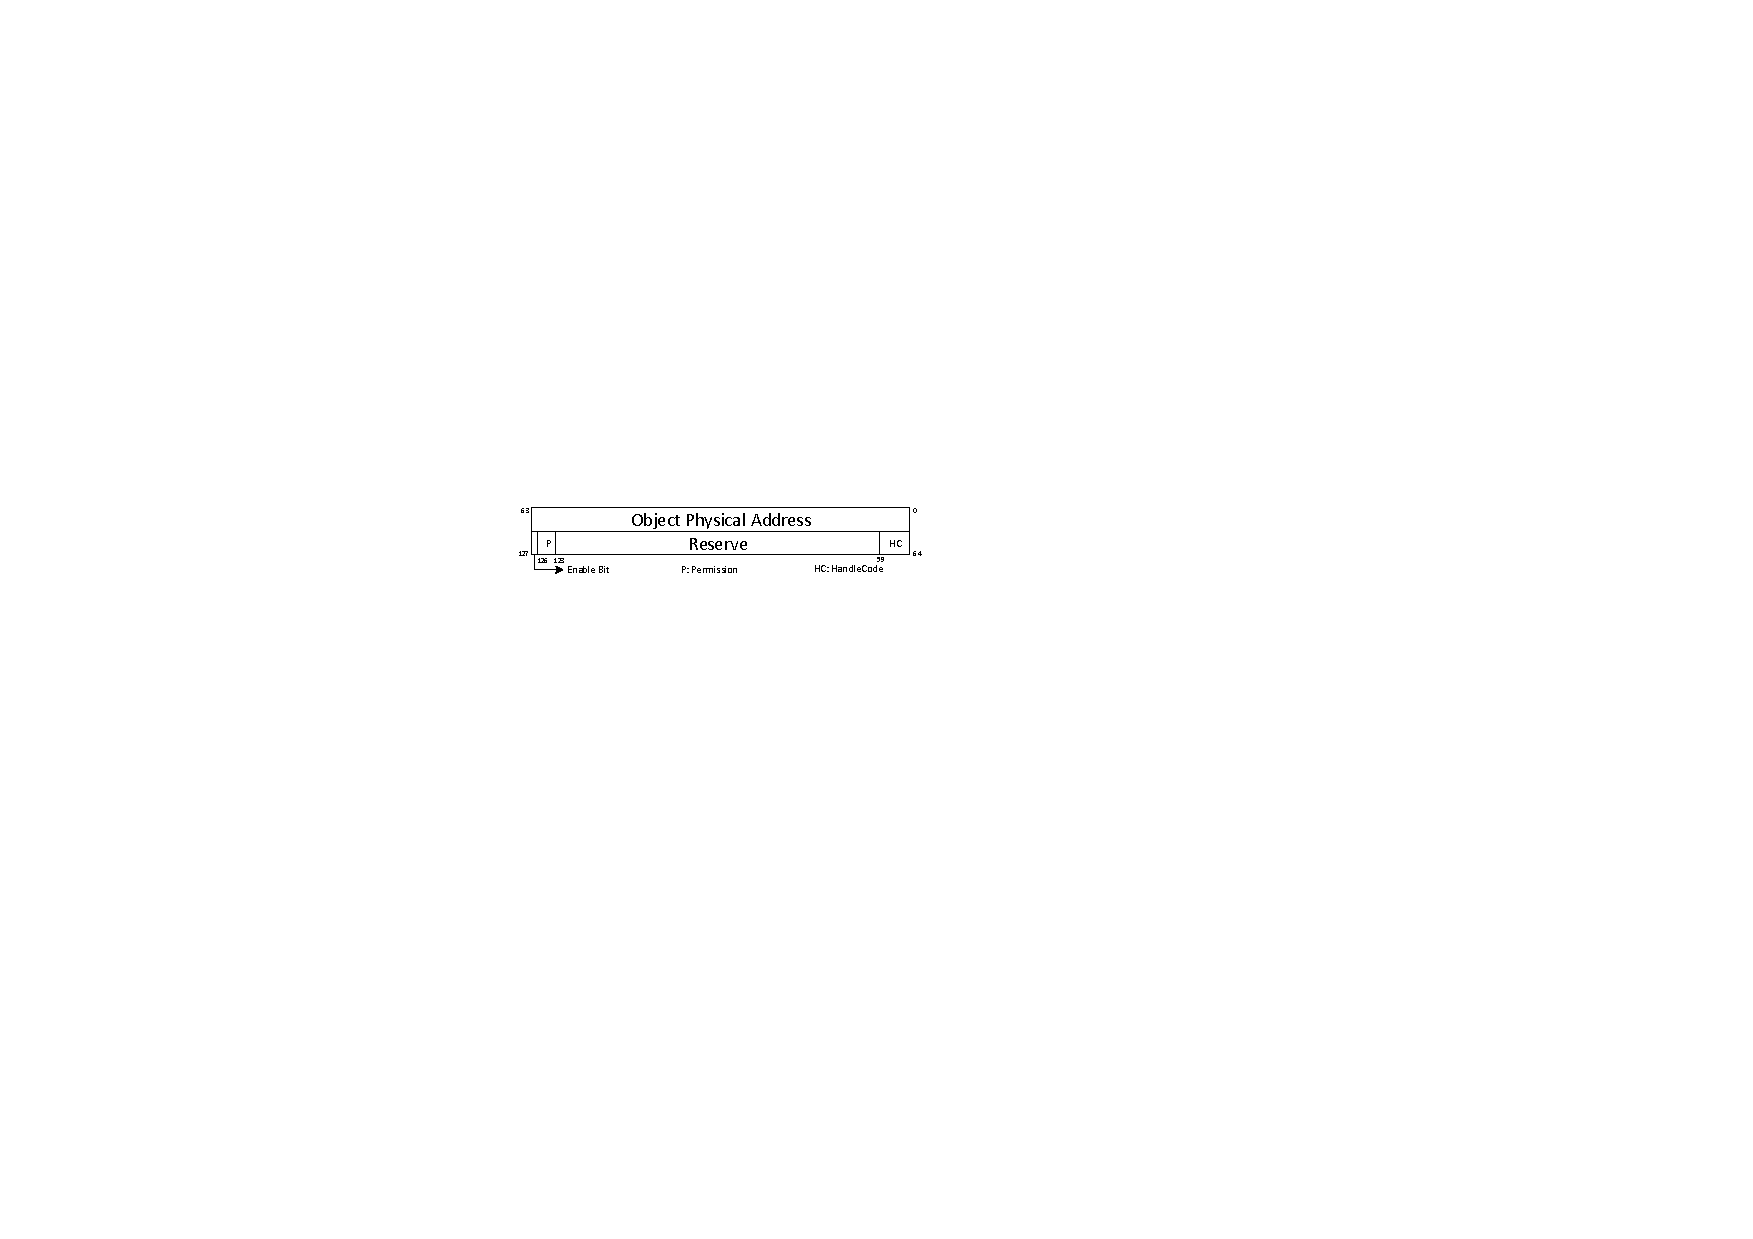
\includegraphics[scale=0.5]{pic/handlerules.pdf}
    \caption{HandleRules}
    \label{rulefigure}
\end{figure}


% Figure \ref{rulefigure} depicts the structure of HandleRules, how KRSA formulates HandleRules and how KRSA use HandleRules to protect the customized kernel.

% Figure \ref{architecture} depicts how KRSA generate HandleRules and uses HandleRules to protect marked kernel objects.
% HandleRules is a new conception put forward by KRSA. Because in different scenario, the protected kernel object varies depending on its scenario, KRSA need a structure to facilitate user designation of protected kernel objects and KRSA  itself implementation of corresponding protection. Figure \ref{rulefigure} depicts the structure of HandleRules.
% KRSA mainly focus on the protection of the customized kernel in a particular scenario, which include kernel code and specific kernel data. Because in different scenario, the protected kernel object varies depending on the scenario in which it it located, KRSA proposes a new concept: HandleRules, to facilitate user designation of protected kernel objects and KRSA implementation of corresponding protection. Figure \ref{rulefigure} depicts the structure of HandleRules.

% HandleRules mainly consists of two parts: the address of protected kernel object and its security attributions.
For the addresses of kernel objects, they are filled by Object Locating Engine at the system initialization stage. The security attributions mainly consist of flags, such as enable bit, permission and HandleCode. Permission indicates the access permission it should set when accessing the protected kernel object. HandleCode is an exception number that is bound to an exception handler, user can choose to declare an exception handler or adopt the system default exception handler while specifying the protected object's HandleRules. 

\subsection{Workflow} \label{section:workflow}
Section \ref{section:frame} has illustrated the four important components in KRSA's runtime framework, this section would detail how different components interact to achieve kernel protection. 

The first step is to formulate all HandleRules as depicted as Path \textcircled{1} and Path \textcircled{2} in Figure \ref{arch}.  When KRSA is started, Object Locating Engine would be the first component to be loaded, as described in Section \ref{section:frame}, when the engine completes a trusted boot, it would formulate HandleRules based on the information tagged on the protected kernel object. 
As described in Section \ref{section:scope}, different kernel objects, especially kernel data, are bound to different labels, so Object Locating Engine needs to adopts different method for different kernel object.

% 在描述完handlerule的定义之后,那么handlerule是如何形成的,又是如何指导KRSA进行保护的,都有哪些保护,在安全违例的时候,又怎么处理。
% 这里需要一个过渡的句子
%正如在section1中所描述的那样,不同的内核对象,特别是内核数据,其别贴上了不同的标签,对象定位引擎需要根据这些标签信息,在系统初始化阶段,首先形成handlerule。
%针对内核代码,第一步,OLE首先读取内核代码段,获取内核代码加载的位置,将地址填入到对应的handlerule中,同时,填入默认的权限位和HandleCode。KRSA默认认为代码段为只读的。其次,遍历整个页表,将参与到内核代码映射的页表项进行标记,按照既定的规则(将在实现部分详细说明)对所涉及到页表项进行设置。最后,通知OPE,通过CR3寄存器获取整个页表的物理地址,对涉及到内核代码的物理页按照既定的规则设置相应的handlerule,KRSA认为代码段(自修改代码单独考虑)是不变的,所以,在对应的handlerule的permission中设置为只读,填入对应的HandleCode。
%针对内核数据,与代码不同,其保护策略一般会随着其所在的场景的不同而不同,所以,其handlerule的形成的过程也不尽相同。首先,OLE读取拥有不同标签的内核数据,然后通过查找系统符号表和页表找到被保护对象的物理地址,记录到对应的handlerule中。其次,在KRSA中,由section 1可以得到,标签一般与权限相对应,所以OLE根据内核数据标签的不同,设置handlerule中对应的permission以及默认HandleCode。KRSA同样允许用户自定义对特定数据结构的处理函数,因此,在这一步中,KRSA提供了接口,在检测到特定对象时,填入的HandleCode将被替为用户自定义的HandleCode。最后,与内核代码设置相似,针对内核数据同样遍历页表,设置相关的页表项,通过CR3等形成相关也表性对应的handlerule。

For kernel code, the first step is that Object Locating Engine reads all the kernel code, gets the locations where the kernel code is loaded. Secondly, Object Locating Engine traverses the whole page tables to find out where kernel code are loaded in physical memory, and fills HandleRules with these addresses, default permission and default HandleCode. KRSA believes that kernel code (except the kernel self-modifying code) should retain read-only and unchangeable. Thirdly, during the process traversing the kernel page tables, Object Locating Engine also finds all page table entries that participate in the kernel code mapping, sets related entries (not limited to the entries that involves in code mapping directly) according to the established rules which would be illustrated in detail in Section \ref{section:handler} 

For kernel data, unlike kernel code, its protection policy generally varies with the scenario in which it is located, so customizable policy must be considered in the process of formulating its HandleRules. Firstly, Object Locating Engine reads the kernel data that has different label, and then finds the physical address of the protected kernel object by using the system symbol table and the page tables. This engine records this physical address into the corresponding HandleRules. Secondly, in KRSA, which has been illustrated in Section \ref{section:scope}, the label generally corresponds to the object's permission, so Object Locating Engine set the corresponding permission bit and default HandleCode in HandleRules depending on the data label. KRSA also allows users to customize the handler for a specific kernel data structure, so in this step, when a particular object is detected (the particular object is bound to its linear address), the HandleCode that is filled in is replaced by the user-defined HandleCode by using an interface provided by Object Locating Engine. Lastly, similar to the kernel code setting, Object Locating Engine also traverses the page table, sets the relevant table entries, and formulates the corresponding HandleRules by hooking CR3. 
%针对运行时新分配的对象,KRSA也做了相应的处理,保护方式也无外乎保护其对象本身和保护其映射方式两种。第一个要解决的问题是其运行时分配问题。KRSA修改了内核源代码,在对象分配过程中,当检测到需要被监控的数据的分配的时候,其会通知Object Locating Engine其新分配的地址,以及默认的权限等信息。然后KRSA一方面与上面提到的数据保护一样,根据分配的地址和权限信息生成该分配对象对应的handlerule,根据页表信息和CR3信息建立对想对应的页表的HandleRules。另外一方面在特定的内存区域中对新分配的对象备份,这块内存由OPE维护,被保护的内核不能访问到。

% For new allocated object in runtime. KRSA provides protection on protecting the object itself and the mapping relationship. The first problem to be solved is the problem of its runtime allocation. KRSA modifies the kernel source code, when the object that should be protected is allocated or initialized, Object Locating Engine would get a signal and obtain the address where the object is allocated as long as the permission and some other information. Then, similar to the handle process of mentioned in kernel data, KRSA formulates the corresponding HandleRules based on address and permission, KRSA also creates the corresponding page table entries' HandleRules based on page table and CR3 information. Lastly, Object Locating Engine would call an interface of Object Protection Engine to back up the newly allocated object in a particular memory area, this memory erea is maintained by Object Protection Engine and it not accessible to the protected kernel.


% \subsubsection{HandleRules Usage}
% 度过系统初始化第一阶段之后,所有被保护内核对象都经由OLE读取,形成了对应的HandleRules,至此,OLE, 作为interface,的初始化阶段的工作已经完成。KRSA使能OPE,来到系统初始化的第二个阶段,根据传入的handlerule形成对所有标注的内核对象的保护。
The second step is depicted as Path \textcircled{3} and Path \textcircled{5} in Figure \ref{arch}. KRSA enables Object Protection Engine to set protection to all kernel objects delivered by HandleRules. As illustrated in Section \ref{section:frame}, Object Protection Engine has the full control of guest kernel memory, thus
% after the first phase of KRSA initialization as described above, HandleRules of each protected kernel objects have been formulated by Object Locating Engine, so Object Locating Engine, as an interface between protected kernel and Object Protection Engine, has completed its work in the initialization phase. Then KRSA enables Object Protection Engine to set protection to all kernel objects delivered by HandleRules. As illustrated in Section \ref{section:frame}, Object Protection Engine has the full control of guesst kernel memory, thus, as depicted in Figure \ref{arch} \textcircled{3} and \textcircled{5},
on receiving the HandleRules, Object Protection Engine would set the memory access permissions for the corresponding kernel object based on the content of the permission bit in HandleRules.
% As illustrated in Section \ref{section:frame}, Object Protection Engine is a component that
Because Object Protection Engine occupies higher privilege than the protected kernel, so the protected kernel cannot violate the access to the memory area that has been protected by Object Protection Engine. KRSA would come to protection stage at the time when all HandleRules have been imported by Object Protection Engine. 

% OPE实时监控对被保护内核对象的访问,当违例发生的时候,即发生了对被保护对象的非法获取的时候,首先,OPE会中断被保护内核的执行,取得控制权,然后根据上下文信息,索引到对应的handlerule中,然后读取其中的HandleCode。其次,根据得到HandleCode,查找异常处理表,然后转移到对应的异常处理程序中,对相对应的非法获取进行处理。针对每种不同的保护对象,或者每一种默认的HandleCode,OPE是如何处理的将在section 2中详细说明。
% Object Protection Engine provides systematical protection to all kernel object delivered by HandleRules at runtime.
At runtime, Object Protection Engine provides real-time monitor on access to protected kernel objects. As depicted as Path \textcircled{4} in Figure \ref{arch}, once violation occurs, the protection mechanism in Object Protection Engine will be triggered. First of all, Object Protection Engine would interrupt the execution of protected kernel, trap into handler process, in this process, Object Protection Engine would index to the corresponding HandleRules according to the context information. Then, be similar to interruption handle in kernel, indexing the HandleCode in HandleRules, Object Protection Engine would transfer to exception handler on the assist of the exception handling table. For the handler to different kernel object or default HandleCode would be illustrated in Section \ref{section:handler}. 


% 当一个内核模块插入到系统的时候,lkm模块负责模块的加载,然后将lkm模块代码与被保护数据的地址以及权限,HandleCode等信息传递给OLE,然后OLE通过系统调用表,页表,CR3的辅助,形成对于LKM模块的代码和数据的handlerule。
In addition, Loadable Kernel Module should be considered because it can introduce kernel objects possessing kernel privilege. As depicted as Path \textcircled{6} in Figure \ref{arch},  when a loadable kernel module is inserted into the system, LKM Protection Module would be actived to load the module, and delivers address of module code and protected data, permissions and HandleCode to Object Locating Engine. On receiving these information, Object Locating Engine formulates HandleRules on assist of system call table, page table and CR3.


% \begin{figure}
%     \centering
%     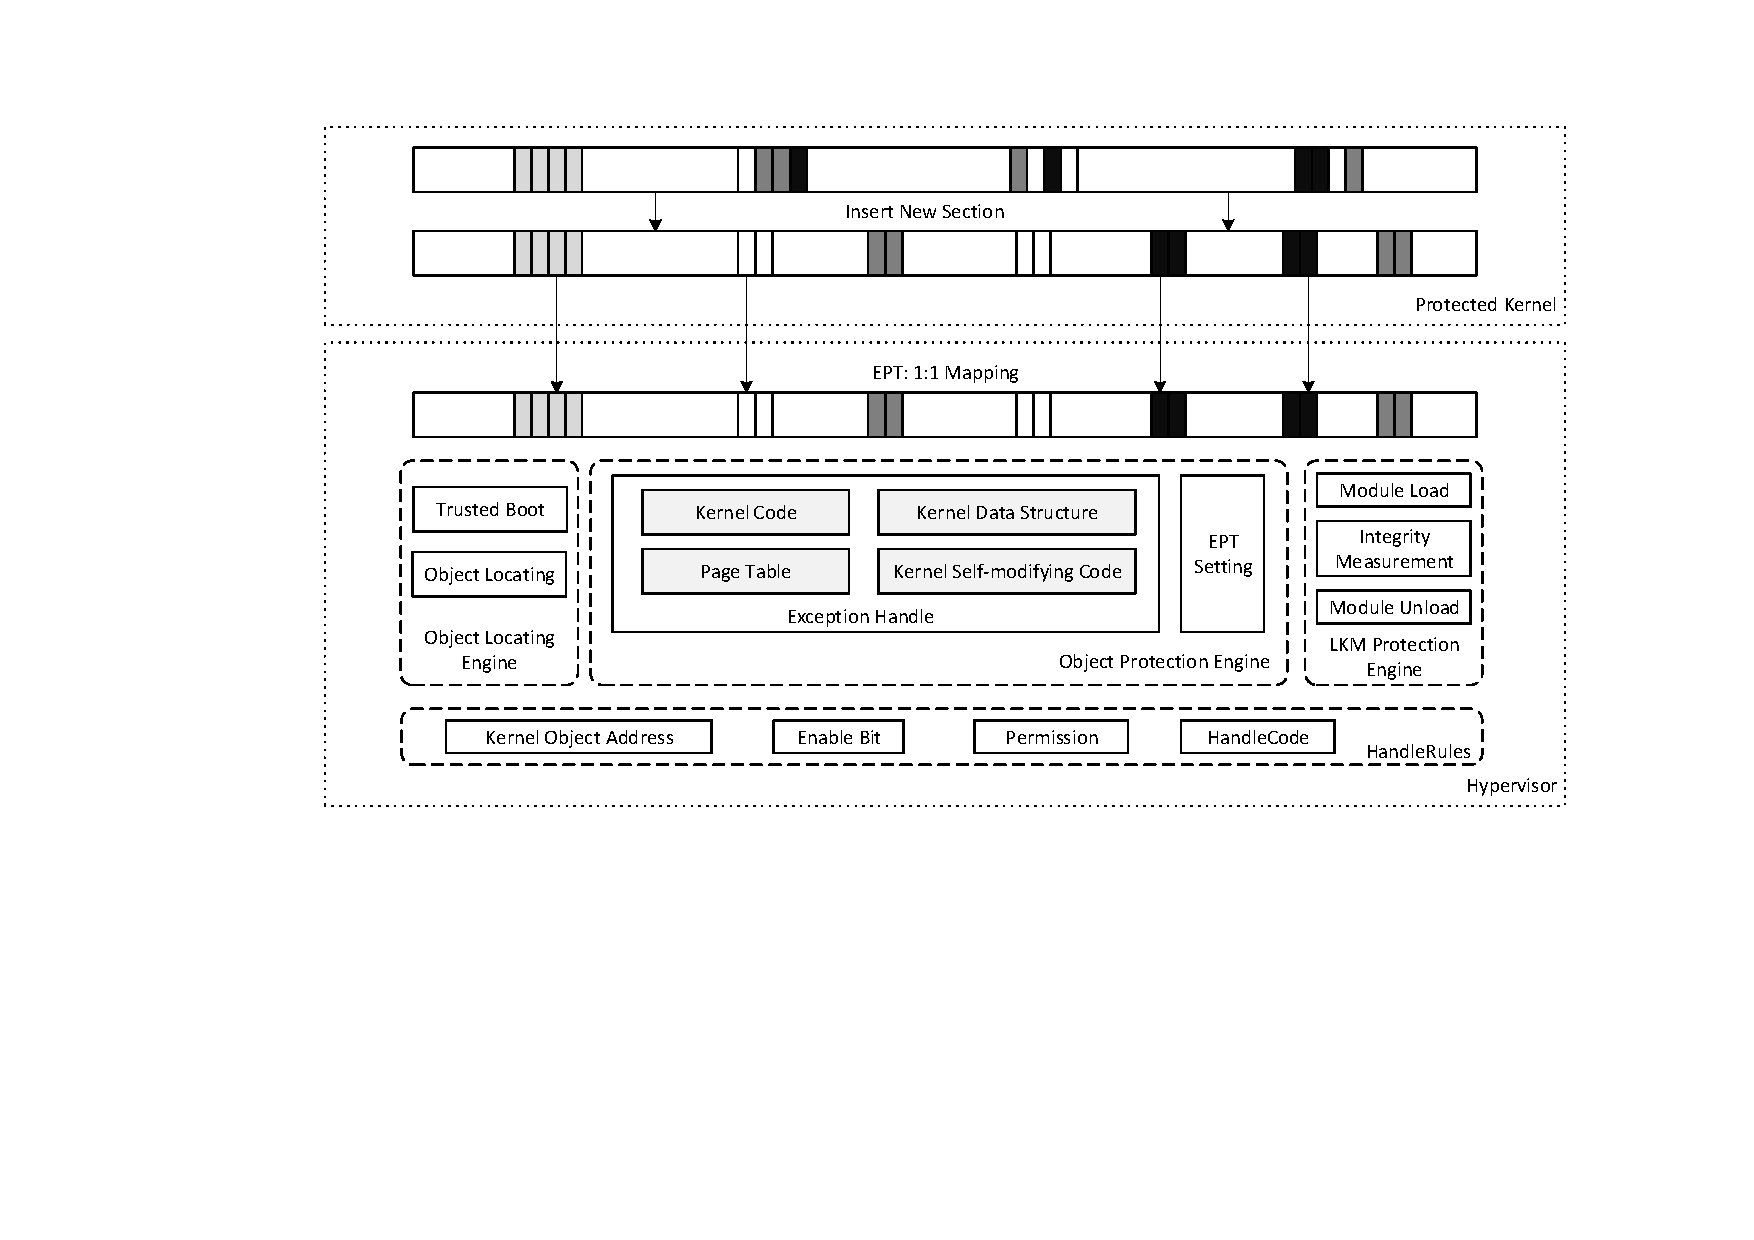
\includegraphics[width=0.85\textwidth,height=0.35\textwidth]{pic/frame.pdf}
%     \caption{Prototype of KRSA on Intel x86 Architecture}
%     \label{frame}
% \end{figure}
%


\fi


% 设计部分,图重新画
% 实现部分的内容,主要是针对上面设计部分提到的具体如何保护的实现,对于数据的标记再详细说明,说明链接脚本。主要包括如何保护内核代码,处理自修改代码的具体的方法,页表的保护方法,页表的写模拟,如何可信启动等内容



\iffalse
\section{Implementation} \label{section:implementation}
% \subsection{Overview}
Figure \ref{frame} depicts our prototype based on Intel x86 hardware virtualization technique. Section \ref{section:aggre} illustrates how Object Locating Engine locates and declares the protected kernel objects. Section \ref{section:handler} illustrates the protection to some objects used by Object Protection Engine. Section \ref{section:trustedboot} how KRSA is loaded with trust.

% KRSA is a systematical architecture can be deployed on the machine based on any instruction set architecture. Here, we achieve a prototype based on Intel x86 hardware virtualization technology. Figure \ref{frame} shows our prototype. KRSA firstly makes little modifications to the protected kernel source code,inserts the custom sections. Secondly, KRSA recompiles kernel source code using a customized linker script which will be illustrated in Section\ref{section:aggre}. Thirdly, KRSA employs a tiny hypervisor as a secur execution environment and deploys and implements the three protection engines mentioned in Section \ref{section:frame} in this hypervisor.

% \begin{figure}
    % \centering
    % 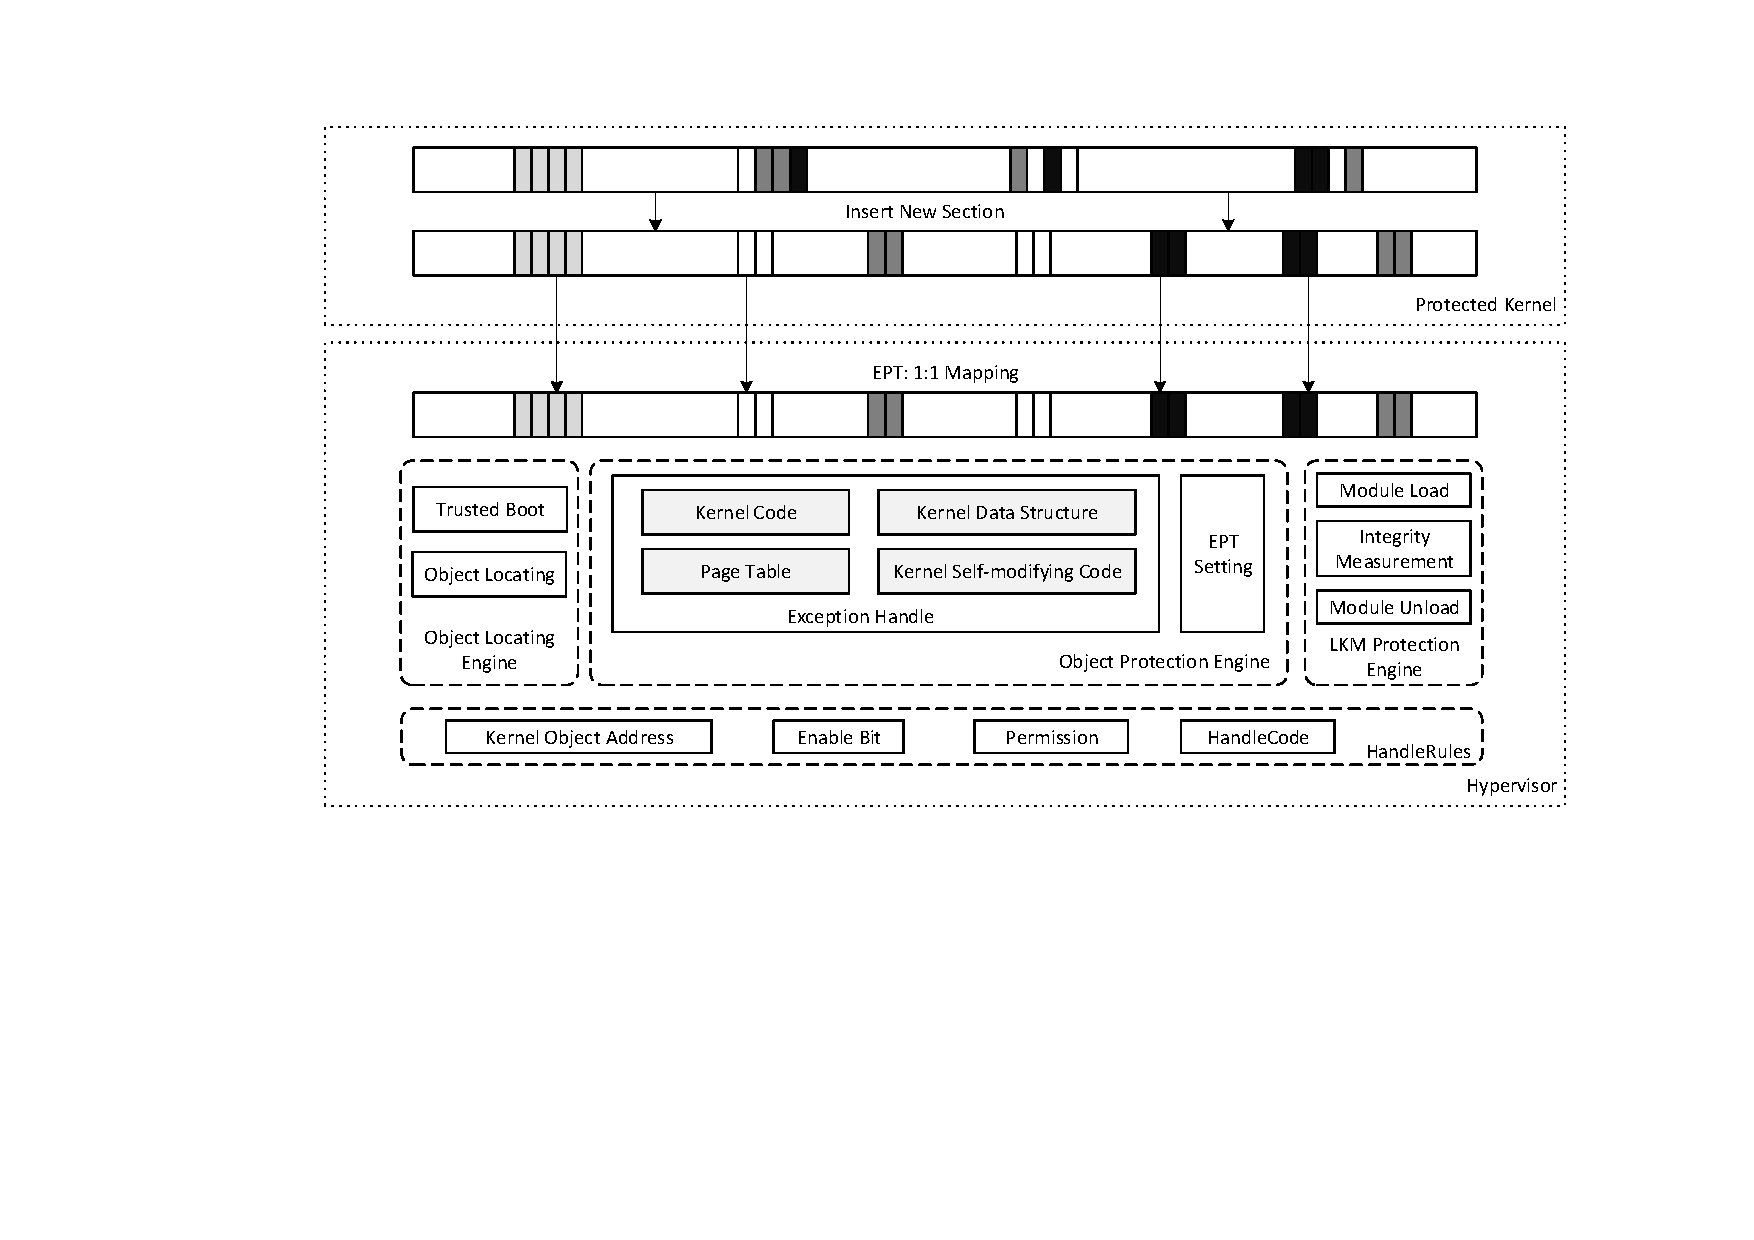
\includegraphics[scale=0.56]{pic/frame.pdf}
    % \caption{Prototype of KRSA on Intel x86 Architecture}
    % \label{frame}
% \end{figure}

%KRSA firstly makes little modifications to the protected kernel source code, and recompiles the kernel using a customized linker script which will be illustrated in Section\ref{section:aggre}. Secondly, under the protected guest kernel, KRSA employs a tiny hypervisor as the safe execution environment, the hypervisor is respond for executing all handling process. 
% The Systematical Protection Mechanism is executed in this hypervisor. Lastly, all exception handle processes are executed in this tiny hypervisor.

\begin{figure}
    \centering
    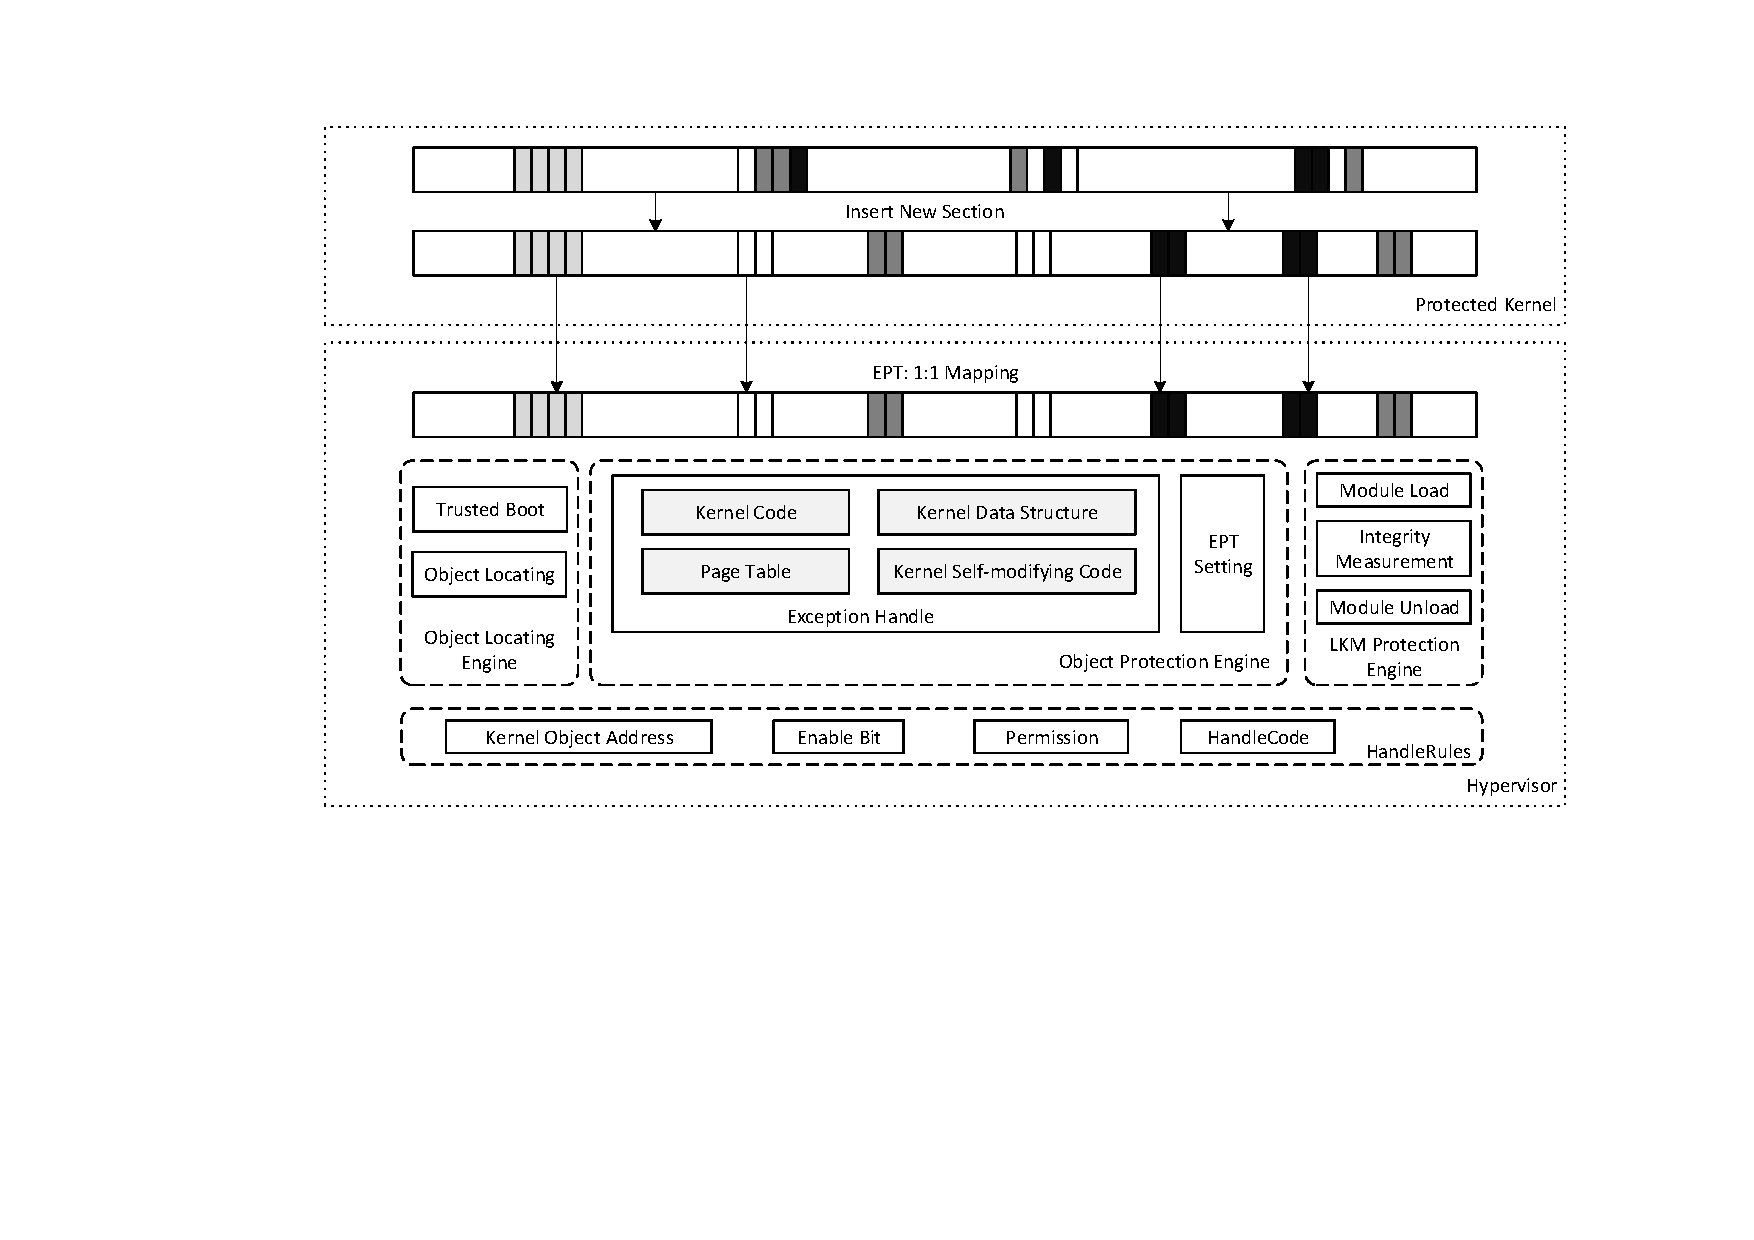
\includegraphics[scale=0.5]{pic/frame.pdf}
    \caption{Prototype of KRSA on Intel x86 Architecture}
    \label{frame}
\end{figure}


\subsection{Object Marking} \label{section:aggre}
% 正如在设计部分所述,针对不同的内核对象,KRSA采用不同的保护策略,不同的内核对象被贴上了不同的标签。这里,实现将着重讲解KRSA是如何对保护对象进行贴标签操作,以及如何将被保护的对象在内存中进行标识。首先,KRSA引入了两个全新的section。data针对的是被保护的一般数据,对这些数据的写操作由KRSA执行。rodata是只读数据,KRSA强化这些数据的只读性质。然后,在源代码中找到对应的数据的声明,添加合乎其权限的section。正如图XXX所示。当所有的被保护的内核对象都已经被声明之后,KRSA使用一个定制的linker对源代码进行重新编译图XXX就是一个链接脚本的一个例子。经过重新编译之后,所有被保护的内核对象都有符合开发者权限要求的标签,并被集中到页对齐的内存中。

% KRSA uses call graph (CG) to identify all key data structure. Firstly, KRSA gets the CG for the customized kernel in the given scenario. In CG, in general, the security module or function we focus on in this scenario is as an end point. Secondly, KRSA uses standard dependency analysis to recursively find each path that end of this end point. In our analysis, each path we get would end with \textit{sys\_call\_table} or \textit{idt\_table}, because KRSA just protect the customized kernel. Thirdly, KRSA formulates all data in the path into a set, and conducts intersection operation to all sets that end with a same end point. Fourthly, KRSA marks the data in all the collections from the third step as data to be protected, but different data need to be protected with different permissions, thus, KRSA uses different label to tag different kernel data. In our preliminary design, the type of labels is related to the type of permission required by the kernel object. Assuming that only RWX(read, write, execution) is considered for data kernel object, KRSA has designed two type of labels: Read-Only, Read-Write.
% 通过上述的X步骤得到的最后的数据集合就是KRSA要保护的数据,这些数据为所有控制流路径上不可绕过的点。一般而言,这些数据都是一些关键的branch数据。因此,保证对这些数据的合法访问,就可以保证在特定应用场景中,被保护的关键功能能被正确使能。
% In fact, the each kernel data obtained through the four step above is a point that cannot be bypassed on all control paths, and these data generally are key bracnch data. Therefore, The legitimate access to these data reinforced by KRSA can ensures that the security module or function protected in a particular scenario can be properly enabled.

As described in the Section \ref{section:scope}, KRSA needs to first find the protected objects and their access permissions. 
KRSA uses Call Graph (CG) to identify all key data structure. Firstly, KRSA gets the CG for the customized kernel in the given scenario. In CG, in general, the security module or function we focus on in this scenario is as an end point. Secondly, KRSA uses standard dependency analysis to recursively find each path that end of this end point. In our analysis, each path we get would end with \textit{sys\_call\_table} or \textit{idt\_table}, because KRSA just protect the customized kernel. Thirdly, KRSA formulates all data in the path into a set, and conducts Conjunction (AND) operation to all sets that end with a same end point. Fourthly, KRSA marks the data in all the collections from the third step as data to be protected, but different data need to be protected with different permissions. In our prototype, only RWX(read, write, execution) is considered for data kernel object, KRSA has designed two type of labels: Read-Only, Read-Write, and introduces two new section: \verb|.ckrsa.data| and \verb|.ckrsa.rodata|. \verb|.ckrsa.data| is used for the protection to these data whose write operations are performed by KRSA. \verb|.ckrsa.rodata| is used to protect read-only data, KRSA enhances the read-only policy of these data. Secondly, in the source code, KRSA find places of the declaration of protected kernel objects and insert the declaration of the section, Figure \ref{declare} give an example on this process. 

\begin{figure}[!htbp]
    \begin{minipage}[t]{0.5\linewidth}
{\tt \small \begin{verbatim}
// security/security.c
    ...
struct security_hook_heads 
security_hook_heads
__attribute__ 
((section (".ckrsa.data"))) = {...} \end{verbatim}
}
    \caption{A Section Attribute Example}
    \label{declare}
\end{minipage}
\begin{minipage}[t]{0.5\linewidth}
{\tt \small \begin{verbatim}
// arch/x86/kernel/vmlinux.lds.S
/* Data */
. = ALIGN(PAGE_SIZE);
.ckrsa.data : 
AT(ADDR(.ckrsa.data) - LOAD_OFFSET)
{ *(.ckrsa.data) }
\end{verbatim}}
    \caption{A Modified Linker Script Example}
     \label{linker}
\end{minipage}
\end{figure}


% \begin{figure}[!htbp]
% {\tt \small \begin{verbatim}
% // arch/x86/entry/syscall_64.c
%     ...
% asmlinkage const sys_call_ptr_t
%     sys_call_table[__NR_syscall_max+1]
%     __attribute__ ((section (".ckrsa.rodata"))) = {
%     ...
% // security/security.c
%     ...
% struct security_hook_heads security_hook_heads
%     __attribute__ ((section (".ckrsa.data"))) = {
%     ...  \end{verbatim}
% }
%     \caption{A Section Attribute Example}
%     \label{declare}
% \end{figure}
%
At last, when all the protected kernel objects have been declared, KRSA uses a custom linker to recompile the source code. Figure \ref{linker} is an example of a linker script. After recompilation, all protected kernel objects would be allocated into page-aligned memory. 

% \begin{figure}[!htbp]
% {\tt \small \begin{verbatim}
% // arch/x86/kernel/vmlinux.lds.S
%     ...
%     /* Data */
%     ...
%     . = ALIGN(PAGE_SIZE);
%     .ckrsa.data : AT(ADDR(.ckrsa.data) - LOAD_OFFSET) {
%         *(.ckrsa.data)
%     }
%     . = ALIGN(PAGE_SIZE);
%     ...  \end{verbatim}
%       }
%     \caption{A Modified Linker Script Example}
%      \label{linker}
% \end{figure}
%



\subsection{Object Protection} \label{section:handler}

% 这部分内容主要讲我们是如何针对不同的保护对象设置不同的HandleRules的。这里涉及到一个问题,就是如何引出页表的保护的内容。这里还是存在一个问题,就是在对象引擎与具体的保护之间存在一个问题,是写引擎的实现还是写具体的保护的实现?写引擎的实现与设计相符合。假如写引擎的实现,其内容在上面已经写了,就是引擎要实现什么功能已经说明了,下面的内容应该是讲具体引擎如何实现。那么引擎的具体实现是什么?就是讲如何获取对象的地址,如何获取对应的权限,当异常放生的时候,如何设置引导到对应的异常处理程序,或者讲如何引导到默认的默认程序中去。这样讲默认的异常处理程序,又是另外一个内容,所以,上面讲异常处理的时候,只能讲通过监控EPT来具体的实现,然后具体的默认异常处理程序是放到新的章节去讲的。
At runtime, as illustrated in Section \ref{section:frame}, no matter what the protected kernel object is, the work of formulating its HandleRules involves page tables. However, it is unnecessary to protect the whole page tables, because the vast of majority of page table entries do not involve protection of protected kernel objects, Object Locating Engine in KRSA also classifies the corresponding page table entries in a precise way based on the nature of the protected kernel object, thus KRSA can protect as few page table entries as possible. Figure \ref{pg} depicts how KRSA classifies page table entries. 

Firstly, with the help of virtualization technology, value loaded into CR3 register is cached and monitored by KRSA, only approved value can be loaded into CR3 register. Secondly, Object Locating Engine clears the write permission for the whole kernel page tables, no matter the page table is involved in translating protected objects or not. Thirdly, Object Locating Engine travels all page table entries and marks different page table entries with different tags. Different tags are involved with the protection to different kernel objects. In our prototype, KRSA divides all page table entries into five categories as illustrated following. 

\begin{enumerate}
\item Code-relevant PTE (E1): If the page table entry involves mapping the kernel code, KRSA will label this page table entry as code-relevant PTE.
\item Data-relevant PTE (E2): If the page table entry involves mapping the protected kernel data structures, KRSA will label this page table entry as data-relevant PTE.
\item Restricted PTE (E3): If any of the page table entries are identified as E1 in a page table, then all remaining page table entries that are not part of E2 will be identified as restricted PTE.
\item Unrestricted PTE (E4): If no page table entry is marked as E1 in a page table, but at least one page table entry is identified as E2, all remaining page table entries in the same page table are identified as unrestricted PTE.
\item Unmonitored page PTE (E5): If a page table entry is not satisfied with any circumstance mentioned above, this page table entry is identified to be unmonitored page PTE.
\end{enumerate}

%讲一下这么标识的原因以及会取得的效果
\begin{figure}
    \centering
    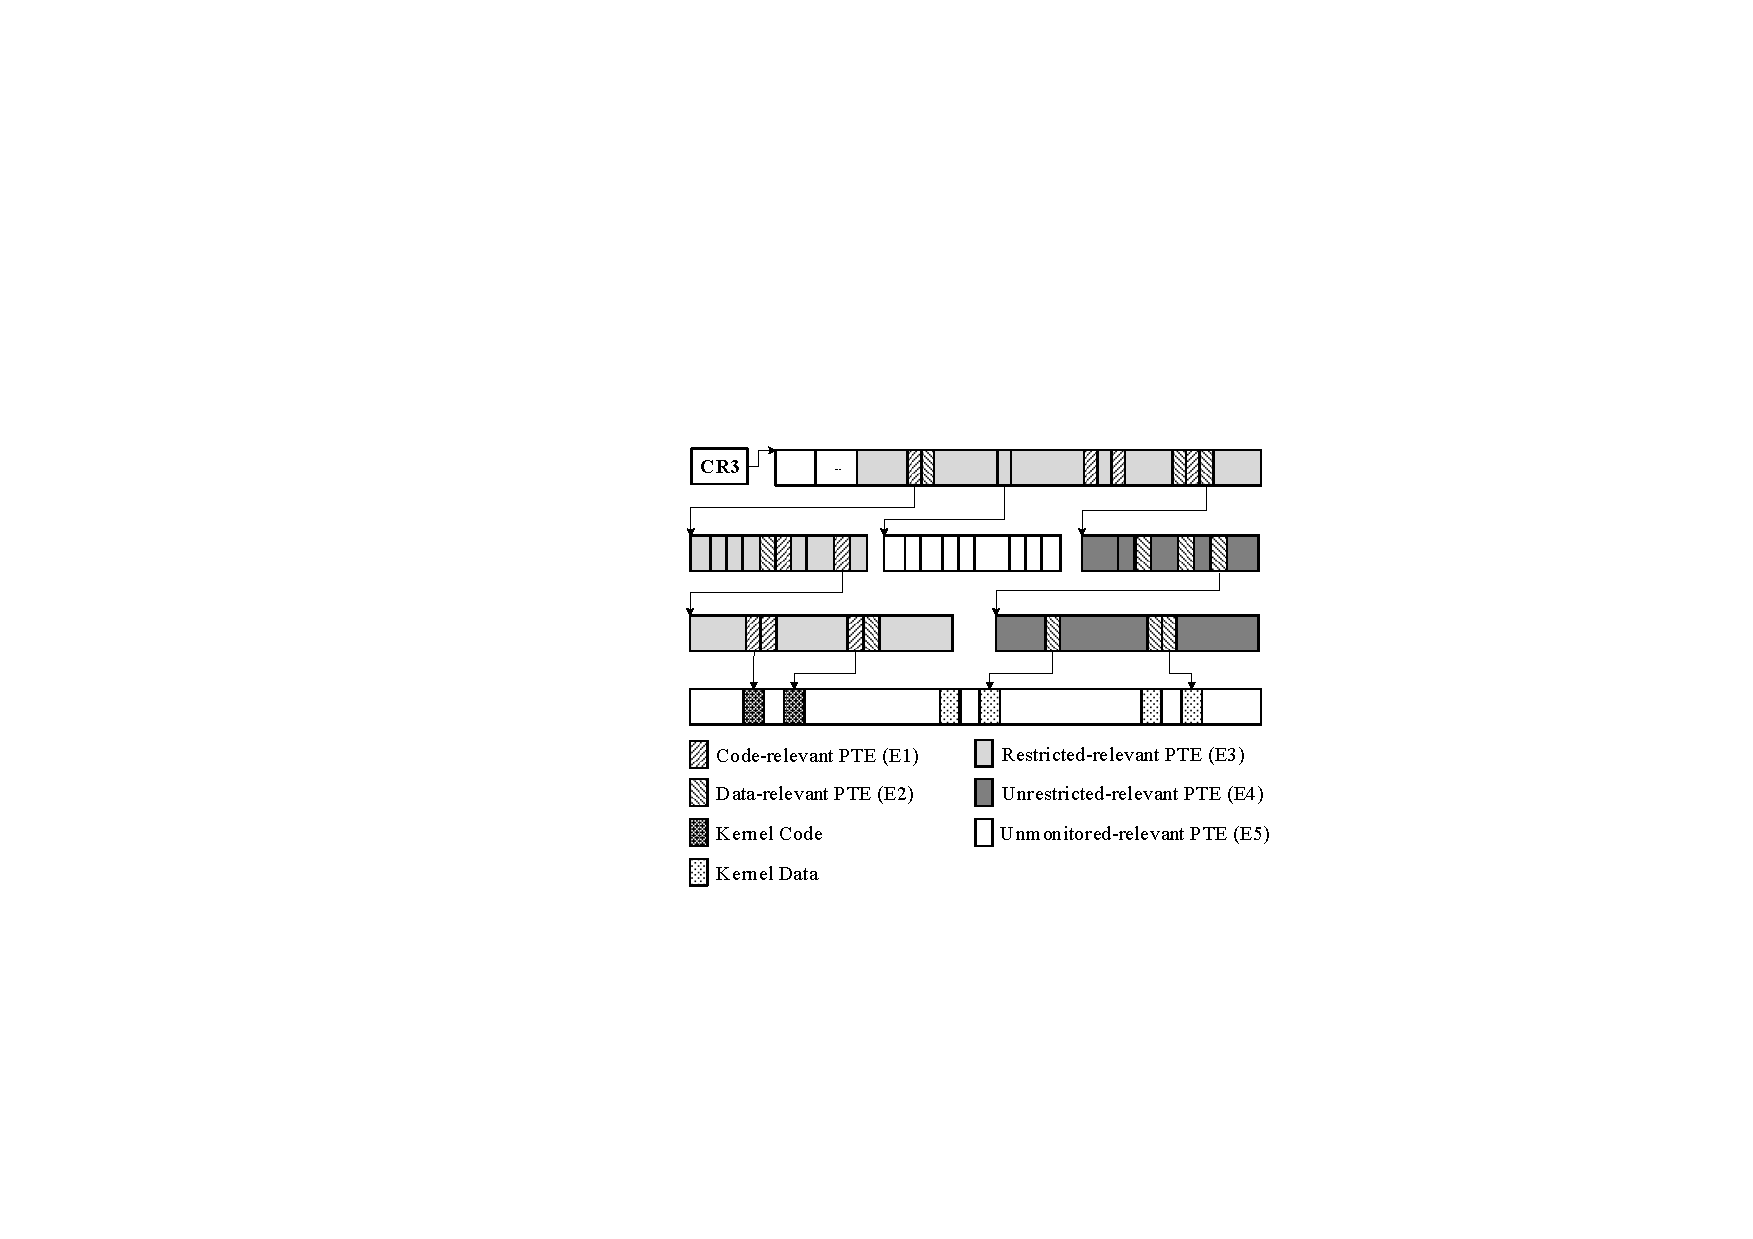
\includegraphics[scale=0.5]{pic/page_table.pdf}
    \caption{An Example of Page Table Entry Classification}
    \label{pg}
\end{figure}



In our prototype, KRSA adopts Extended Page Table (EPT) with 1:1 mapping relationship to monitor the protected kernel memory. During initialization stage, Object Protection Engine set EPT entries according to the information in HandleRules. Then this engine would handle security violations according to HandleCode in the HandleRules at runtime. 
% KRSA also developes some default HandleRules for some kernel objects, the kernel object that need to be protected in all scenarios would adopt default HandleRules.

\paragraph{Kernel Code}
KRSA maintains the integrity of the kernel code from two aspects. On the one hand, Object Protection Engine would reject any modification to kernel code, on the other hand, Object Protection Engine would protect kernel code relevant page table entries to prevent double mapping and remapping attack. 
Firstly, Object Protection Engine monitors and rejects any write operation to these memory range containing kernel code. Object Locating Engine removes write permission in page table entries associated with kernel code, and Object Protection Engine reinforces this policy in associated EPT entries, thus when someone wants to subvert kernel by modifying kernel code, Object Protection Engine would always capture this operation and reject it with the help of tiny hypervisor. Secondly, Object Protection Engine also prevent the adversary from adding or deleting code, this work is accomplished by protecting page table entries that belong to E1 and E3 as illustrated in the above paragraph. 
For PTEs that marked to be E1, they are involved with translation of the kernel code. KRSA need to guarantee that the adversary can not modify these PTEs to replace kernel code with unauthorized one. So Object Protection Engine would reject the operation of modifying code-relevant PTEs with the help of hypervisor. 
% If someone tries to write a PTE marked to as E1, Object Protection Engine would force virtual machine exit and reject that operation with the help of tiny hypervisor.
For PTEs that marked as E3, they should be considered because these PTEs share the same page with PTEs belonging to E1. KRSA must prevent an adversary from converting a data page to a kernel code page. 
% Unfortunately KRSA doesn't know the information of processes, it can't know whether a page is used as a code page or a data page, so KRSA can't limit the execution of pages.
% KRSA set the NX bits in the kernel page table entries whose level is as high as possible. Because once the NX bit is set in any level page table entries, the related page can't be executed anymore in the multiple level paging structure. These PTEs actually belong to E3.
Thus when PTE that belongs to E3 is modified, Object Protection Engine would reject this operation if it adds execution permission to that PTE or change NX bit. 
% Thus when write operation to E3 occurs, Object Protection Engine forces virtual machine exit and checks if this operation adds execution permission to that PTE or change NX bit.


\paragraph{Kernel Self-modifying Code}
At runtime, kernel code are not maintain unchangeable because of some kernel feature.
% In general, kernel codes aren't alternated during runtime. However, there are some kernel features actually modifying kernel codes at runtime.
So KRSA adopts special HandleRules to deals with these codes. At runtime, any modification to kernel code would force virtual machine exit, and Object Protection Engine would search all HandleRules to find out whether the VM-Exit matches a kernel self-modifying code`s HandleRules or not. In our prototype, KRSA formulates four kind of HandleRules for different kind of Kernel Self-modifying Code. 

Statc Keys is used for less branch prediction. When kernel code is modified, in the handler to this kind of kernel self-modifying code, KRSA would force Object Protection Engine to check if a code address in an array named \textit{jump\_entry} matches the address of the modified instruction. If matches, Object Protection Engine would authorize the operation of this instruction.  


% Static Keys swaps between \verb|NOP| instruction and \verb|JUMP| instruction to switch branches instead of condition instructions for less branch predictions. KRSA forces Object Protection Engine to search an array of \textit{jump\_entry} structure which contains the address of the code which could be modified for a jump entry matching the address of the modified instruction. If Object Protection Engine doesn't find it, Object Protection Engine regards the modification isn't caused by this feature, which would trigger further another HandleRules to check or reject this operation. Swapping instructions is a complex process which needs the involvement of INT3 instruction, so Object Protection Engine defines a state machine to judge each step. According to the current instruction and the modification, Object Protection Engine gets a state and a state transition. If the transition doesn't satisfy the requirement of state machine, Object Protection Engine regard the step is illegal. Moreover, for a modification to \verb|JUMP| instruction, Object Protection Engine compares the instruction target and the jump target indicated by the jump entry. If they doesn't match, Object Protection Engine regards the modification is illegal.

KGDB would replaces a instruction with \verb|INT3| to set a breakpoint, when a instruction is replaced with \verb|INT3| instruction, Object Protection Engine would records the original bytes. When \verb|INT3| instruction is modified, Object Protection Engine would check if the address of this modification is recorded before, if not, Object Protection Engine would regard that operation illegal. 

% KGDB is a kernel debugger which replaces original instructions with the \verb|INT3| instruction to set breakpoints. KRSA allows modification to the \verb|INT3| instruction and just records original bytes and the addresses of the modifications. When \verb|INT3| instructions are modified, Object Protection Engine retrieves the records. If Object Protection Engine doesn't find a record where the address and the byte match the address and the byte of the modification, Object Protection Engine regards that operation is illegal.

Ftrace is an internal tracer which alternates the instructions at the beginning of functions. Object Protection Engine interfaces with Object Protection Engine retrieves the kernel symbol table to judge whether the modification is at the beginning of functions. 
% The same with Statc Keys, Object Protection Engine defines a state machine to judge the steps of swapping between \verb|NOP| instructions and \verb|CALL| instructions. The targets of \verb|CALL| instructions include some tracer functions which Object Protection Engine find according source code analysis and trampoline functions. The trampoline functions are dynamically generated depending on a function template. And the difference between them is a jump address in the end. So Object Protection Engine compares the trampoline function and the function template to ensure only the jump target is different and the target is one of functions which Object Protection Engine finds according to source code analysis.

Kprobes uses the INT3 instruction and Ftrace to change the control flow for collecting information.
In generally, Kprobes only uses \verb|INT3| instructions like the way KGDB uses. So Object Protection Engine adopts the same check method with KGDB\@.What's more, Kprobes has an optimizer which replaces \verb|INT3| instructions with JUMP instructions, so Object Protection Engine does checks like what it does in Ftrace. 
% does checks like what it does in KGDB\@. What's more, Kprobes has an optimizer which replaces \verb|INT3| instructions with JUMP instructions. The jump targets are also some trampolines, so Object Protection Engine does checks like what it does in Ftrace\@.

Alternatives alternates codes according to features of processors at runtime. All code modifications caused by the feature rely on another data structure. Fortunately, these modifications are done at boot time of the kernel, so it's unnecessary for KRSA to check them.
% KRSA doesn't support BPF too, because BPF introduces user space codes, KRSA can't judge whether the modification is malicious or not. Fortunately, BPF is usually used in packet filter. Furthermore, if \verb|KGDB| \verb|Kprobes| and \verb|Ftrace| are not supported in practical scenario, KRSA may turn off  relevant protection mentioned above.

\paragraph{Kernel Data Structures}
KRSA uses the method similar to kernel code protection to protect the kernel data structures. 
As mentioned in Section \ref{section:scope}, different kernel data structures with different property are predefined into different sections, and these sections are allocated into different page-aligned memory. Thus, Object Protection Engine just monitors and protects the content in these page-aligned memory by setting corresponding access permissions on EPT entries. Then access without right permission would be trapped into the hypervisor and Object Protection Engine trigger protection defined by HandleCode in HandleRules. 
% the protection method in Object protection Engine. Object Protection Engine would handle these virtual machine exit according to the HandleCode defined in HandleRules.
Be similar to kernel code protection, KRSA also protect kernel data from two aspects: protecting the data memory region and protecting the mapping relationship. 
For the first aspect, for kernel data structures that are defined into section \verb|ckrsa.rodata|, with the help of tiny hypervisor, Object Protection Engine rejects any write operation to them. Object Protection Engine would handle access without right permission to data structures in \verb|ckrsa.data| according to HandleCode in corresponding HandleRules too. 
% Be similar to data structures in \verb|ckrsa.rodata|, access wihout right permission to data structures in \verb|ckrsa.data| would be trapped into hypervisor too. Object Protection Engine handles these access according to actions defined in HandleRules.
For the other aspect, KRSA also protects data-relevant page table entries as illustrated above to reinforce the security in protecting kernel data structure, this process mainly involves E2 and E4 in the Classification of page table entry. 
% For fault access to PTEs belonging to E2, KRSA just forces virtual machine exit and handles these PTEs, because these PTEs are involved with protected data.
Object Protection Engine rejects modification to the memory regions that contain PTEs who belong to E2. This guarantees the mapping relationships invariable to prevent the adversary from modifying these data structures illegally or replacing them with a fake one.
The PTE that belongs to E4 is protected because it shares the same physical page with the PTE that belongs to E2, so Object Protection Engine would be triggered and emulate the write operation if a PTE that belongs to E4 is written. 
% If a PTE belongs to E4, it actually doesn't invoke with the translation of protected kernel objects. But they share the same page with PTEs that belong to E2, thus hypervisor will force virtual machine exit too, when write operation occurs to that  page frame containing PTE belongs to E2. So KRSA must emulate the write operation to PTEs that belong to E4 in hypervisor.

\paragraph{Loadable Kernel Module}
Loadable Kernel Module is a special case should be protected, because it can introduce new kernel code and data structures. In details, KRSA implements two hypercalls to deal with the addition and reduction of LKM code. By modifying the kernel source code, hypercall would be called if the protected kernel is going to load or unload a kernel module. In KRSA, LKM Protection Engine would receive these hyeprcalls to accomplish load and unload work in hypervisor. 
Firstly, LKM Protection Engine would verify the integrity of the core text and initialization text of the module before the kernel module initialization function at the time protected kernel is going to load a kernel module. 
Secondly, LKM Protection Engine would inform Object Locating Engine to modify the permission of the last level page table entries of module regions, KRSA deprives these page table entries with execution permission. In this step, LKM Protection Engine has not load LKM core code into kernel space. This step mainly prevents attacker from executing data pages. Thirdly, LKM Protection Engine loads LKM code into kernel space and forces Object Locating Engine to modify the kernel page table entries to restore the lost execution permission and correct the execution permission in high level page table entries. Object Locating Engine also constructs corresponding HandleRules just as the engine does for original kernel code.  
Data structures introduced by LKM is protected with similar steps. 
% If the developer want to protect some data structures imported by this LKM, developer just formulates the customizable HandleRules, then KRSA would load these HandleRules and protect these specified data structure.
On receiving the second hypercall, LKM Protection Engine would interface with Object Locating Engine to clear all execution permissions of the kernel PTEs which are related to the unloaded codes. This prevents any succeed execution of the module code.

%
% \begin{figure}
%     \centering
%     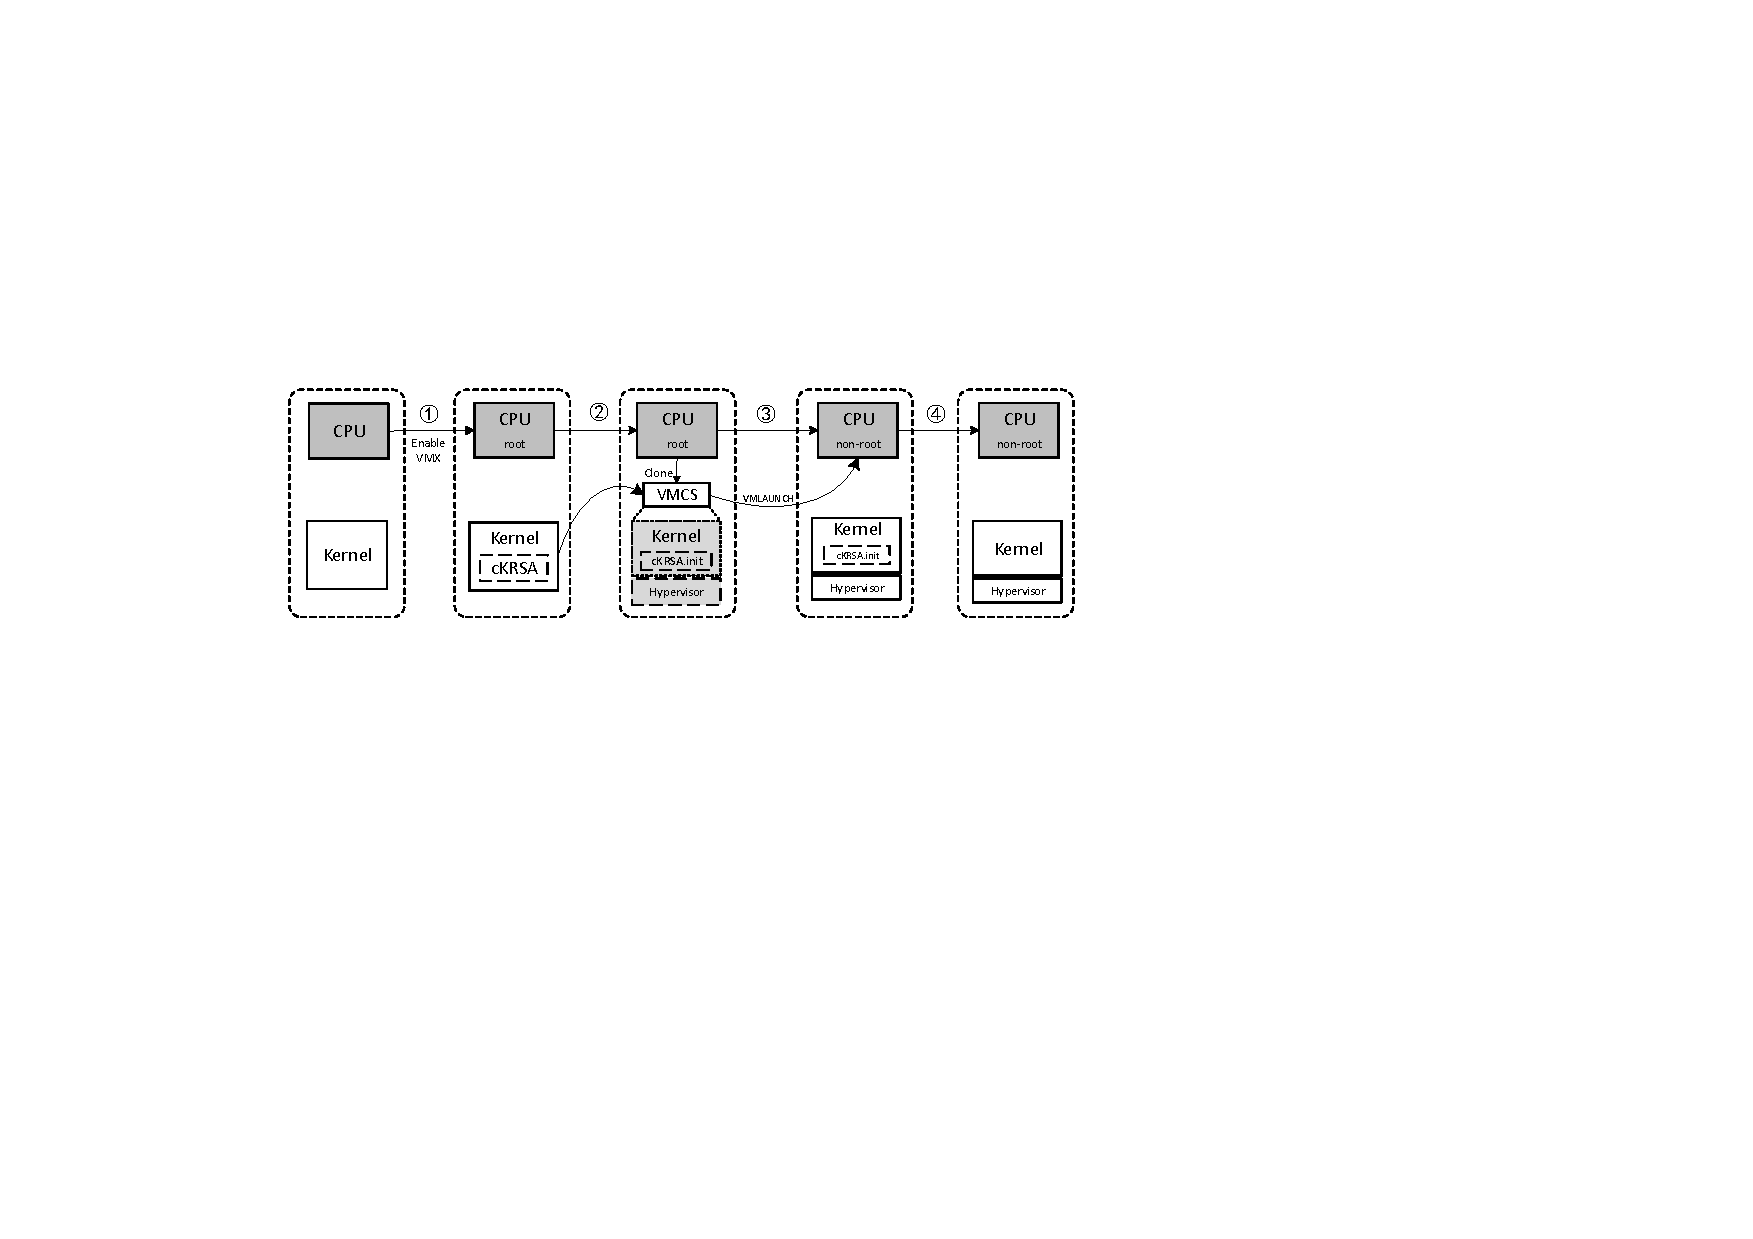
\includegraphics[width=0.85\textwidth,height=0.2\textwidth]{pic/delayedboot.pdf}
%     \caption{The Process of Delayed Boot}
%     \label{db}
% \end{figure}



\subsection{Trusted Boot} \label{section:trustedboot}
% Because KRSA mainly focuses on runtime protection, and with the help of Intel TXT\cite{txtintel}, KRSA does not involve the boot process of the protected kernel. However, when the kernel initialization is completed, KRSA will be loaded as the first loadable kernel module, therefore, KRSA must ensure its own trusted boot.
In security environment, the linux kernel usually is trusted boot with the help of TPM, because KRSA aims at providing the runtime protection, it does not interface with the boot process of the kernel. When the kernel initialization is completed, KRSA will be loaded as the first loadable kernel module and convert the protected kernel into a VM, therefore, KRSA must ensure its own trusted boot.
% KRSA provides runtime systematical protection to the customized kernel, thus KRSA does not involve the boot process to protect the kernel, actually, as described in Section \ref{section:frame}, KRSA would be the first kernel module to loaded after the kernel boot, thus KRSA must be loaded with trust.
% In order to ensure that KRSA can be loaded with trust, Object Locating Engine implements the loading process as shown in Figure \ref{db}.
Firstly, Object Locating Engine in KRSA would check and enable hardware virtualization and request memory from the protected kernel to store KRSA relevant code and data and build a new memory mapping for them in proper memory address space after all memory regions have been allocated. When all the work mentioned above is complete, KRSA will enable VMX. Secondly, similar to the general virtualization startup process, Object Locating Engine initializes and set the VMCS region. Thirdly, VMLAUNCH would be called to launch the virtual processor, the protected kernel would run in the non-root mode. Lastly, Object Locating Engine would load other engines into memory and enable them. So far, KRSA is trusted to be loaded into the execution environment. 


%多核支持
% \subsection{Multi-Core Support}
% Nowadays, most processors have multiple cores.
% For performance and compatibility, we support multicore.
% Like most systems with multicore support, KRSA provides some exclusive data for each core and solves resource sharing problem.
% Though KRSA uses only one set of EPT paging structures, the core has owned translation lookaside buffers (TLB).
% TLBs are updated automatically, so once a core modifies EPT entries, it uses inter-processor interrupts (IPI)
%  to broadcast the modification to all other cores to flush their TLBs.
% If not, there is a case that a core can modify a page and another core can execute the page at the same time.
% Thus, KRSA virtualizes IPIs. If an IPI is generated by KRSA, KRSA handles the IPI. Otherwise, the IPI is delivered to the guest.


\fi

\iffalse

\section{Evaluation}

\subsection{Security Analysis}
KRSA focuses on key kernel objects which mainly consist of kernel code and kernel structures. In order to measure the security of KRSA, we choose the attacks shown in Table \ref{table:attacks} to attack a system protected by KRSA. 
% In this paper, we provide a systematical protection on various kernel objects including kernel code and kernel data structures. So that, as long as the developer pre-defines what data structures should be protected and what actions should be set to protect them, KRSA can provide a solid security enhancement. We choose the following attacks showed in Table \ref{table:attacks} as examples to measure the security of KRSA, because the attack targets pose extreme importance to kernel security and protected by KRSA.

\begin{scriptsize}
\begin{table}[h!]
  \centering
  \caption{Attack Cases}
  \begin{tabular}{c|c}
    \hline
    \textbf{Attack Name    } & \textbf{Attack Behavior} \\
    \hline
      sk2rc2  & Sys\_call\_table[\_NR\_oldolduname] \\
    \hdashline[.4pt/1pt]
      eNYeLKM 1.2 & kernel code modification \\
    \hdashline[.4pt/1pt]
      Adore-ng-2.6  & proc fs file operations table \\
    \hdashline[.4pt/1pt]
      SucKIT-2 & Interrupt descriptor table \\
    \hdashline[.4pt/1pt]
      POSTER & Master Kernel Page Table \\
    \hline
    \end{tabular}
  \label{table:attacks}
\end{table}
\end{scriptsize}

% By analyzing the behavior of these attacks, we find that the adversary can subvert the OS kernel in two ways: by modifying kernel data or by modifying kernel code. KRSA builds solid security enhancement on both ways to achieve systematically protection.
By analyzing the behavior of these attacks, KRSA enhances the protected kernel from two aspects: maintain invariant of kernel code and protect kernel data. 

At first, for kernel code, with an elaborate on attacks, adversary tampers the kernel code by using the following three methods. The first kind of attack such as \verb|NYeLKM|, Because the protected kernel can not access to EPT which is maintained by the hypervisor with a higher privilege, on the one hand, write to the memory region that contains kernel code would always be captured and rejected by Object Protection Engine. On the other hand, page table entries who are involved in mapping kernel code 

Firstly, kernel data can be subverted using the following two method. The first kind of attack such as \verb|POSTER|, the adversary can subvert the kernel by using a forged fake kernel data. KRSA deprives the kernel with the capability of modifying the corresponding page table entries, so any write operation to relevant page table entries would be trapped into the hypervisor and handled by Object Protection Engine according to HandleRules. The second kind of attack such as \verb|SucKIT-2| and \verb|sk2rc2| subverts the physical memory region that containing protected kernel data. Because the protected kernel can not access to EPT which is maintained by the hypervisor with a higher privilege, write to this memory region would always be captured and rejected by Object Protection Engine. 

Secondly, for kernel code, with an elaborate on attacks, adversary tampers the kernel code by using the following three methods. The first kind of attack such as \verb|NYeLKM|, the same with what the attack does in data attack, conduct double mapping or re-mapping attack to subvert the kernel code in memory, thus both of these two aspects are reinforced by KRSA with the similar protection method. \verb|Adore-ng-2.6| is an attack instance for the second kind of attack, adversary subverts the kernel with an illegal LKM. LKM Protection Engine conducts integrity measurement to guarantee the LKM loaded into the kernel is authorized by KRSA. For the last kind of attack to kernel code, the attacker can use virtual dynamic shared objects to executing userspace code with kernel privilege. KRSA employs protection mechanism such as ASLR, DEP/NX, SMEP to guard kernel code. 


% Firstly, we can prevent attacker from modifying the key data from two aspects. For the first aspect, the attacker can forge a fake data structure, then subvert the kernel to use the fake one, this kind of attack doesn't modify the real data but subvert the kernel successfully. One attack instance is POSTER. So KRSA deprives the kernel with the capability modifying the protected page table entries. Thus any operation to write these page table entries is authorized by KRSA, any attempt to write relevant protected kernel page tables will be trapped into the tiny hypervisor and disposed according to HandleRules.  For the second aspect, the attacker can tamper the kernel data structures on physical address directly, or the attacker can use double mapping to the protected kernel data structures. For this kind of attack such as SucKIT-2 and sk2rc2, KRSA let Object Protection Engine monitor the physical pages containing protected data Structures. Therefore the security of selected kernel data structures will be guaranteed by KRSA perfectly.

% Secondly, we guarantee that any code in kernel space is authorized by KRSA. After an elaborate analysis on these attacks on kernel code, we find that the attacker can tamper the kernel code using the following three methods. For the first kind of attack method, the attacker can modify the kernel code directly the same with the attacker dose in data attack. NYeLKM is a attack instance for this kind of attack. KRSA adopts the same protection method with data protection, mapping relationship and guest physical content are protected by Object Protection Engine. For the second kind of attack which conduct attack as Adore-ng-2.6 does, the attacker inserts a vicious LKM into kernel space. KRSA provides two hypercall to ensure that only authorized LKM can be loaded into kernel space. Integrity Measurement Engine would firstly calculate the kernel module, if the result is not satisfied with the result of the official kernel module, KRSA would forbid this kernel module to be loaded into the kernel. For the last kind of attack to kernel code, the attacker can use virtual dynamic shared objects to executing userspace code with kernel privilege. KRSA employs protection mechanism such as ASLR, DEP/NX, SMEP to guard kernel code.


% Please add the following required packages to your document preamble:
% \usepackage{multirow}
\begin{table*}[htbp]
\centering
\caption{Performance Comparisons Using LmBench}
\resizebox{\textwidth}{15mm}{
\label{table:lmbench}
\begin{tabular}{|c|c|c|c|c|c|c|c|c|}
\hline
    \multirow{2}{*}{\textbf{Index}} & \multicolumn{3}{c|}{\textbf{Context Switch}} & \multicolumn{5}{c|}{\textbf{System Call}}         \\ \cline{2-9} 
                                & 2p/16k      & 8p/16k    & 16p/16k   & null call   & fork proc   & sh proc     & open close & stat     \\ \hline
Native                          & 0.713       & 1.096     & 1.266     & 0.293       & 93.2        & 2163.33     & 1.080      & 0.733    \\
KRSA                           & 0.965       & 4.470     & 4.670     & 0.295       & 110         & 2430.5      & 1.135      & 0.735    \\ \hline
\hline
    \multirow{2}{*}{\textbf{Index}} & \multicolumn{8}{c|}{\textbf{Communication Bandwidths}}                                            \\ \cline{2-9} 
                                & pipe        & AF Unix   & TCP       & File Reread & Mmap Reread & Bcopy(libc) & Mem write  & Mem read \\ \hline
Native                          & 6159.666    & 6575      & 4679      & 6802.7      & 12.7        & 7626.166    & 7540.667   & 12       \\
KRSA                           & 6 5672.5    & 5909      & 4205.5    & 6733.85     & 12.5        & 7682.4      & 7519.5     & 11       \\
\hline
\end{tabular}
}
\end{table*}




\subsection{Performance Evaluation}
In order to test the performance of KRSA, we deploy KRSA on a Levono desktop computer with an Intel I5-4950T CPU and 8GB RAM. 
The architecture is implemented on ArchLinux with kernel 4.2.5. For a given terminal scenario, SELinux is widely used which bases on Linux Security Modules (LSM), in this scenario, after the elaborate analysis using Call Graph,  \textit{security\_hook\_heads} is chunked into section \verb|.ckrsa.data|, \textit{ia32\_sys\_call\_table}, \textit{idt\_table}, \textit{debug\_idt\_table},\newline\textit{trace\_idt\_table} are chunked into section \verb|.ckrsa.rodata|, and KRSA adopts HandleRules that have formulated before to protect these kernel objects. 
% KRSA aims at this security scenario as the target and analyses key kernel data structures. KRSA chooses to protect the LSM, at this scenario, \textit{security\_hook\_heads}, \textit{security\_hook\_list} are chunked into \textit{Optional Protected Group}. \textit{sys\_call\_table}, \textit{ia32\_sys\_call\_table}, \textit{idt\_table}, \textit{debug\_idt\_table},\textit{trace\_idt\_table} are chunked into \textit{Basic Protected Group}. In this scenario, we just formulate HandleRules to forbid any write operation to object no matter they belong to \textit{Basic Protected Group} or \textit{Optional Protected Group}. Under the target environment, all performance tests are shown as following:



% \paragraph{Micro Benchmark Evaluation}
Table \ref{table:lmbench} shows the result of the performance overhead introduced by KRSA compared with the native OS. As shown in the table, because of KRSA mainly focuses on kernel objects loaded into the memory, little performance overhead on Communication Bandwidths is introduced. Besides, System Call without frequent process operation, for example \textit{null call}, \textit{stat} and \textit{open close}, performs acceptable which only introduces at most 5\% performance overhead. 
Because of hardware limitation (the experimental CPU only has four cores, four CR3 cache queues), as the number of processes increases, the performance overhead of Context Switch becomes more and more significant, when the perform overhead seems to be acceptable in 2p/16K item. some System Call, such as \textit{fork proc} and \textit{sh proc} performs poorly due to the same reason with Context Switch. However in terminal environment, unlike server environment, ordinary work does not involve with frequent process operations. 
% We use lmbench to examine the performance overhead introduced by KRSA compared with the native OS. The result is shown in Table \ref{table:lmbench}. Memory operations achieve almost as the same performance as the native OS. Also, KRSA poses almost no influence on I/O operations and networking communication. For these I/O related test items such as \textit{open close} , KRSA poses at most 5\% performance overhead, and for these network related test items such as \textit{slct tcp} , KRSA poses at most 1\% performance overhead.
% This is because I/O and network are not the targets should be protected according to our threat model, as the result, hypervisor in KRSA does not virtualize these two aspects. However, operations such \textit{context switch},\textit{fork proc} and \textit{sh proc} seem to gain performance loss. In detail, KRSA also gain an acceptable overhead in 2p/16K text item, when the process come into 8 or 16, the performance seems to be large. The reason is that our CPU has only four cores and four CR3 Cache Queue, the hardware can not cope with tasks beyond its hardware core numbers. The reason why items such as \textit{fork proc} and \textit{sh proc} perform poorly with about 14\% overhead on average is as the same as the reason in \textit{context switch}, because all these tests involve with context switch. However in desktop environment, little work requires frequent context switch.
% From the results, we can conclude that KRSA has little performance overhead in most of test items, and KRSA can be applied into the desktop environment.


% \paragraph{Application Performance Evaluation}
We use SPEC CPU 2006 to test the application performance overhead introduced by KRSA compared with the native OS. The result is shown in Figure \ref{spec}. 
Most of items (\textit{bzip2}, \textit{perlbench}, \textit{hmmer} and \textit{gcc}) that can be used on a daily use gain about 2\% overhead on average. KRSA introduces acceptable performance overhead for most of ordinary works in desktop environment. Some applications require large memory allocation such as \textit{mcf} encounter relatively large performance losses wiht 17\%, this is because page table entries are modified frequently which would cause KRSA check the operation frequently. \textit{astar} and \textit{omenttpp} encounter performance loss because of frequent context switch. However for a ordinary use in terminal environment, these applications are not routinely used on a daily basis, so the performance introduced by KRSA is acceptable.  

\begin{figure}
    \centering
    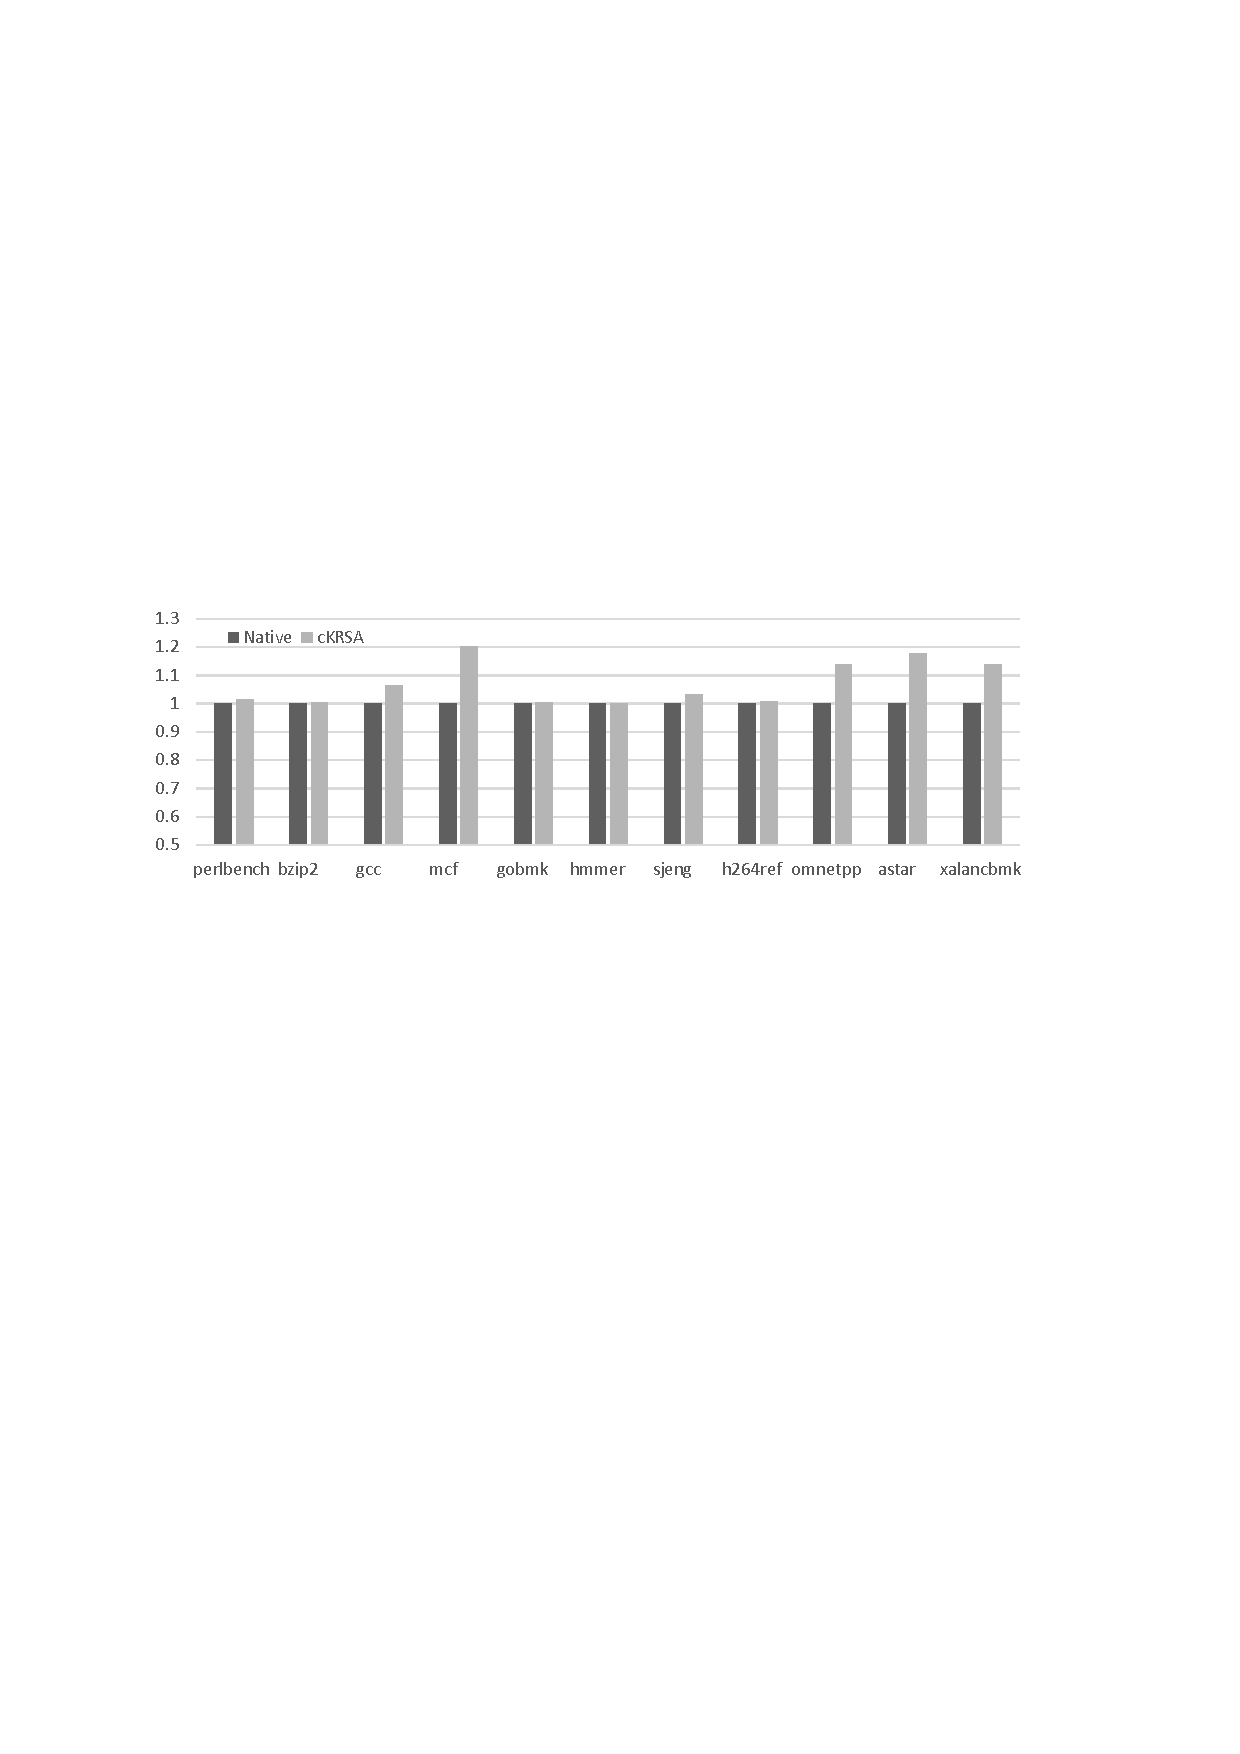
\includegraphics[scale=0.5]{pic/spec_1.pdf}
    \caption{Performance tests using SPECCPU 2006}
    \label{spec}
\end{figure}




% For most items such as \textit{bzip2}, \textit{perlbench}, \textit{hmmer} and \textit{gcc}, they gain about 2\% overhead on average. Ohter items such as \textit{mcf}, \textit{astar} and \textit{omenttpp} have some performance influence with less than 17\% performance loss. \textit{mcf} requires large memory to run, KRSA monitors operation to page tables, though we just part of page tables, when large memory is required, the relevant page table entries will increase, therefore performance loss is caused because security violation. However in ordinary works in desktop environment, few application requests large memory allocation frequently. Some test items such as \textit{astar} and \textit{omenttpp} require frequent context switch. These items are also rarely used in desktop environment. On concluding that, for most of ordinary works in desktop environment, KRSA achieves an acceptable performance overhead.

% \begin{figure}
%     \centering
%     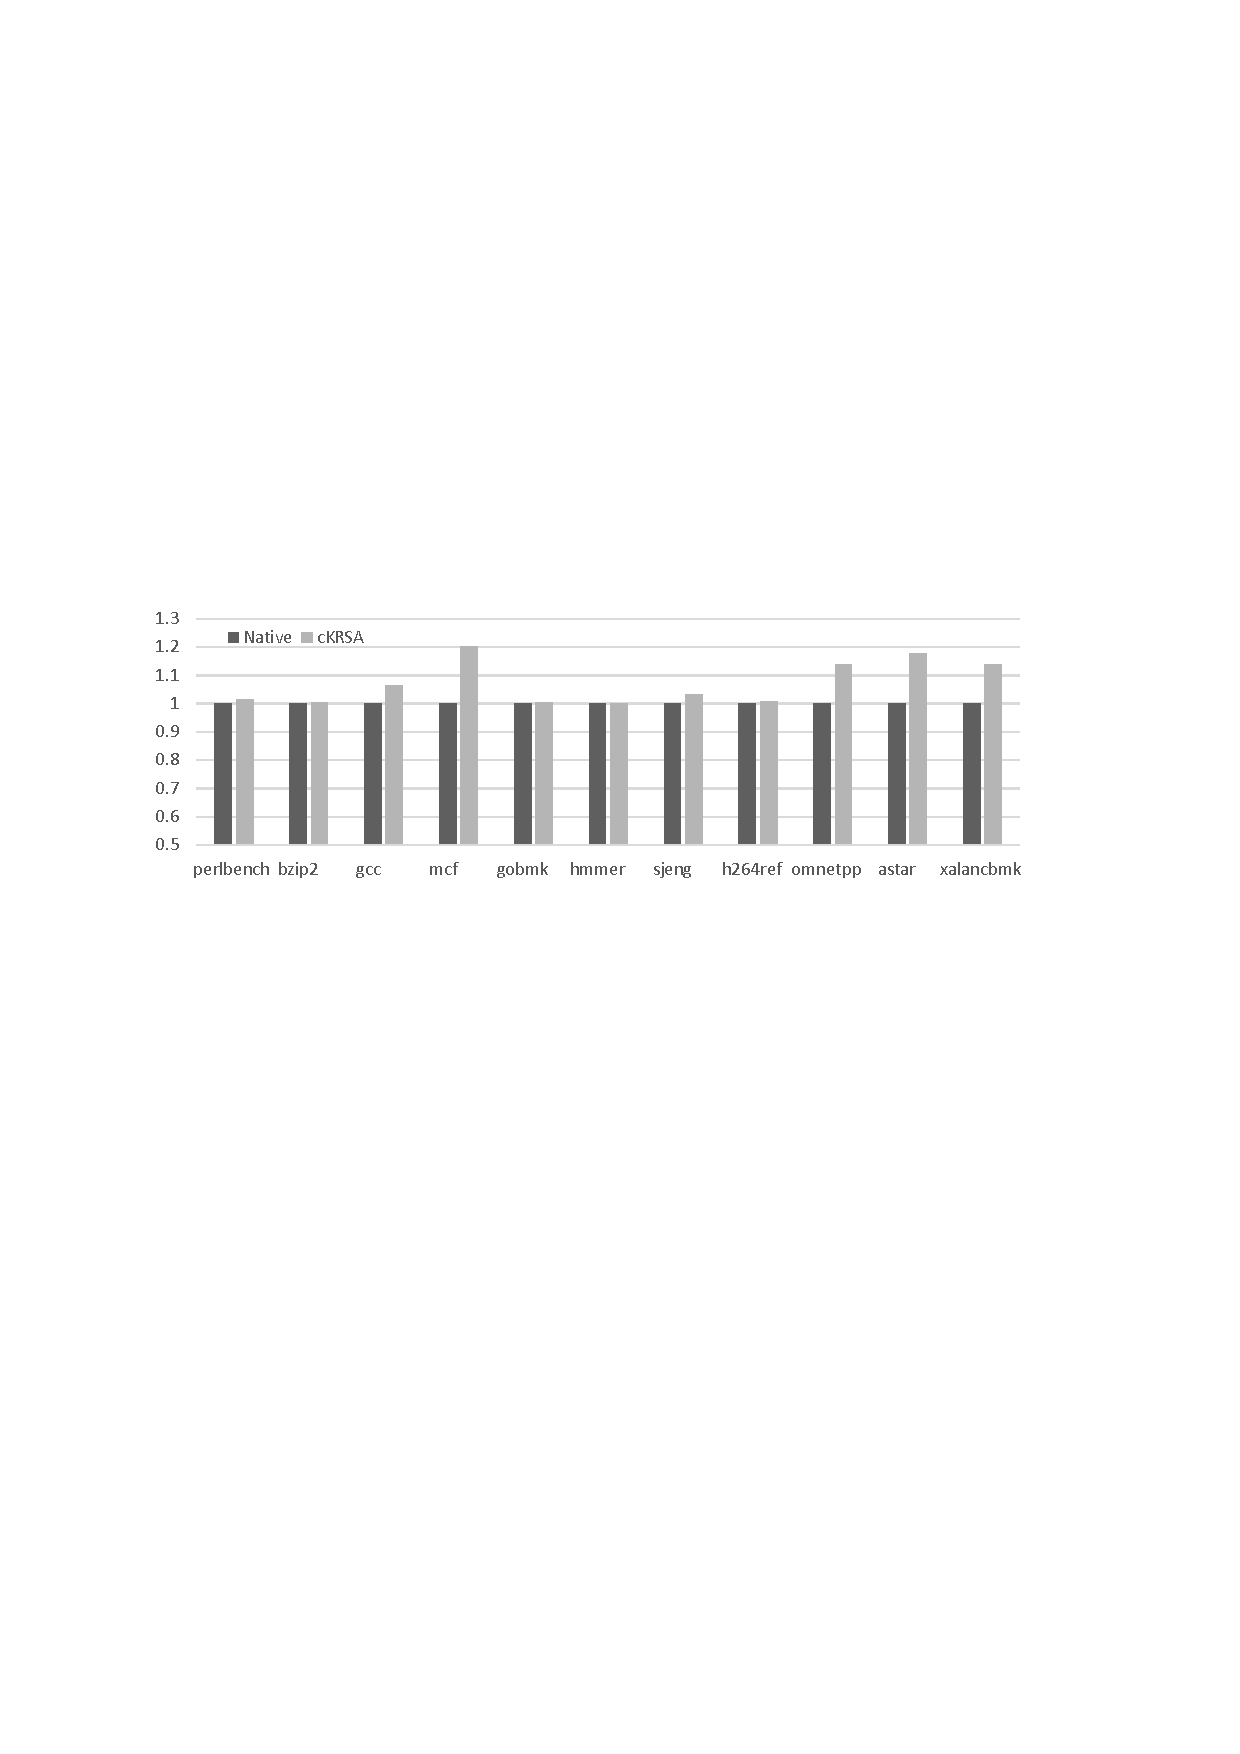
\includegraphics[scale=0.58]{pic/spec_1.pdf}
%     \caption{Performance tests using SPECCPU 2006}
%     \label{spec}
% \end{figure}

\fi

\iffalse

\section{Limitation}
% KRSA is a systematical protection architecture for a customizable scenario. We have shown its conception through experiments with a prototype. However the current prototype of KRSA is not at its full maturity. We describe the limitations of the current prototype in this section.
KRSA is a customizable kernel runtime security architecture to provide systematical kernel protection, covering kernel code and kernel data, in a given terminal scenario. Kernel code is protected from being modified, added and deleted by the methods provided by KRSA. KRSA also prevents adversary from executing code in userspace with kernel privilege. Kernel data however faces more complex protection situations, in general, data can be divided into two types: statically-allocated and dynamically-allocated kernel data. If the kernel data is declared and initialized before the kernel running, such as \textit{sys\_call\_table}, KRSA does provides a series of methods to protect the integrity of the data. However, dynamically-allocated data usually allocated in stack or heap, it would cost much if the detect them during runtime, and direct protection to them with hypervisor also incurs huge performance loss. 
Some complex and subtle availability attacks such as ROP, JOP, DOP mainly leverage those dynamically-allocated kernel data to compromise the kernel, KRSA could only raise the threshold for such attacks through the protection of critical statically-allocated kernel data who is also important for control flow integrity. We will continue to protect against attacks that aim at dynamically-allocated data and control flow on the basis of existing work in the further work. 
% Kernel data can be classified into two categories\@: statically-allocated and dynamically-allocated. For any statically-allocated data structure, KRSA guarantees their security through monitoring the memory region containing them. However some dynamically-allocated kernel data structures are also somewhat important to kernel security. dynamically-allocated data structures can be classified into two class: \textit{control component} and \textit{data component} \cite{osck}. 
% \textit{data component} such as lists of processes and kernel modules usually can be indexed with a fixed head node. so KRSA can use Object Locating Engine to find out the last node in this list, as long as KRSA monitors the integrity of the last item in the list, any write operation to this list can be monitored and protected with KRSA. However \textit{control component} usually is the hook pointing to a kernel function, the hook is allocated in stack or heap. KRSA can not able to prevent these attacks aimed at these data structures.
% Adversary can subvert the kernel by hijacking control flow, KRSA currently can just prevent a few kind of control-flow attacks, but can not solve this kind of attacks completely. Some control-attacks aim at changing statically-allocated control data such as \textit{system\_call\_table}, this kind of attack can be prevent by KRSA completely. Some attacks aims at \textit{data component}, can be somewhat solved as mentioned above. KRSA currently has little effect on preventing some control-flow attacks aims hooks. Besides KRSA works bad on presenting these control-flow attacks which don't change any kind of data structure or kernel code, such as ROP, JOP.
% Future work would be done aimed at preventing attacks on dynamically-allocated data and control-flow.
%
%KRSA also can not prevent the system from ROP or related attacks, but some related works to defeat this kind of attacks have been put forward based on VMM.



%大家都认为保护分为三部分:代码数据和控制流,某些完全解决,某些XXX样。ROP 有抑止作用,但是没有完全解决的能力。
% \textit{Context Switch Performance Loss}:
\fi

\iffalse
\section{Related Work}
Regardless of how the attack changes, it must eventually be settled into the kernel code and kernel data, thus various protection schemes are proposed to address these attacks. 
Some works(OSck\cite{ensosck}, Stider GhostBuster\cite{strider}, VMwatcher\cite{outbox}, HyperTap\cite{invariant}) propose hypervisor-based solution to detect rootkit that compromise the kernel. Some hardware-assisted solutions, such as Copilot\cite{coplilot}, Vigilare\cite{vigilare}, Ki-Mon\cite{ki-mon}, introduce an additional hardware to monitor memory or take snapshots of the memory to detect if the protected kernel is compromised. In contrast, KRSA is for the prevention of kernel rootkits execution in the first place by protecting the predefined data structures and kernel text from being manipulated by them.

SecVisor\cite{secvisor}, Patagonix\cite{hyperbina} propose some security enhancements, such as PXN/SMEP, implemented by using software methods have been replaced by the hardware mechanism applied in KRSA. In order to protect kernel, Lares\cite{secarch}, Nested kernel\cite{nest15} and PT-Rand\cite{ptrand} pay attention to kernel page table, which is shared with KRSA, but KRSA achieves our protection requirements and better performance by only protecting just a part of page table entries. 

Some solutions inspire us to implement KRSA, NICKLE\cite{vmmshadow} uses memory shadowing and instruction emulation to protect kernel code, while KRSA protects kernel data as well and achieves a better performance with the help of hardware. HookSafe\cite{hooksafe} mainly focuses on protecting kernel hooks and control flow integrity, while KRSA emphasizes on protection to the selected kernel objects involved with security threaten in a given scenario.
% pays attention to the integrity of kernel code and critical kernel data to protect the security functions and modules in a given scenario.
Nested kernel\cite{nest15} implements the same protection purposes, but requires the user to be fully aware of the kernel and has the ability to modify kernel, whereas KRSA only requires users to be able to identify the objects they want to protect and locate them in source code. In the process of implementing KRSA, we also draw on a series of protection schemes for our tiny hypervisor, including formal verification\cite{sel4,sel413} , security enhancements \cite{memsafe,hypersentry,hyperSafe}, and size reduction \cite{break,nova,seccloud}.

\fi

% %\subsection{Self-Protection and Prevention}
% \subsection{Hypervisor-based Protection}
%
% %The first area of related work includes recent efforts in enforcing kernel integrity to thwart kernel rootkit installation or execution. To ensure kernel code integrity, techniques such as driver signing \cite{drisign}, Limbo \cite{simrootkit,detrootkit} have been proposed requiring each kernel driver to be digitally signed by a trusted entity and the kernel loading process will verify the digital signature and refuse to load unsigned drivers. Several alternative operating system designs provide privilege separation and memory isolation, including microkernels \cite{SPIN}, ExoKernels \cite{dune}. However, such approaches abandon commodity OS design. Moreover they implement in the same TCB as the untrusted kernel, leaving them potentially to be bypassed. In comparison, KRSA operates at the lower VMM level and is able to blocking kernel-level malicious code inject.
%
% %[2] Driver Signing for Windows. http://www.microsoft.com/resources/documentation/windows/xp/all/proddocs/en-us/code_signing.mspx?mfr=true.
%
% %[30]Christopher Kruegel, William Robertson, and Giovanni Vigna. Detecting Kernel-Level Rootkits Through Binary Analysis. In Proceedings of the Annual Computer Security Applications Conference (ACSAC), December 2004.
%
% %[47]Jeffrey Wilhelm and Tzi cker Chiueh. A Forced Sampled Execution Approach to Kernel Rootkit Identi[1]cation. In Recent Advances in Intrusion Detection (RAID 2007), September 2007.
%
% %[8]A. Belay, A. Bittau, A. Mashtizadeh, D. Terei, D. Mazires, and C. Kozyrakis. Dune: Safe user-level access to privileged CPU features. In Proceedings of the 10th USENIX Conference on Operating Systems Design and Implementation, OSDI’12, pages 335–348, Berkeley, CA, USA, 2012. USENIX Association.
%
% %[9]B. N. Bershad, S. Savage, P. Pardyak, E. G. Sirer, M. E. Fiuczynski, D. Becker, C. Chambers, and S. Eggers. Extensibility safety and performance in the SPIN operating system. In Proceedings of the Fifteenth ACM Symposium on Operating Systems Principles, SOSP ’95, pages 267–283, New York, NY, USA, 1995. ACM.
%
% Many mechanisms have been proposed to protect the kernel with the hypervisors, because hypervisors with the higher privilege than the OS kernels are capable of investigating the kernel memory and intervening the kernel events. Among them, SecVisor \cite{secvisor}, NICKLE \cite{vmmshadow} and Patagonix \cite{hyperbina} are closely related to our work. SecVisor is a tiny hypervisor that simulates the PXN/SMEP by setting and augmenting the page tables whenever the CPU enters or exits the kernel. In addition, SecVisor also checks certain kernel states upon mode switch, e.g., return from a system call. However, the deployment of SecVisor requires many modifications to OS kernel source code. NICKLE is a guest-transparent solution that uses memory shadowing to store a duplication of authenticated kernel code. But NICKLE is based on instruction emulation, which introduces a heavy overhead. Patagonix provides hypervisor support to detect covertly executing binaries. Due to the lack of hardware supports, these mechanisms have higher performance overhead when compared with KRSA, which also use hardware PXN/SMEP. PerspicuOS \cite{nestkernel} enforces the same policies, but it can be invoked much more efficiently via direct nested kernel operations instead of expensive hypercalls. Compared to KRSA these systems do not protect kernel hooks from being subverted to compromise kernel's control-flow.
%
% %[25]Arvind Seshadri, Mark Luk, Ning Qu, and Adrian Perrig. SecVisor: A Tiny Hypervisor to Guarantee Lifetime Kernel Code Integrity for Commodity OSes. In Proceedings of the ACM Symposium on Operating Systems Principles (SOSP), October 2007.
%
% %[26]R. Riley, X. Jiang, and D. Xu. Guest-Transparent Prevention of Kernel Rootkits with VMM-Based Memory Shadowing. In RAID ’08: Proceedings of the 11th International Symposium on Recent Advances in Intrusion Detection, 2008.
%
% %%[27]L. Litty, H. A. Lagar-Cavilla, and D. Lie. Hypervisor Support for Identifying Covertly Executing Binaries. In Security ’08: Proceedings of the 17th USENIX Security Symposium, 2008.
%
% %[24]Dautenhahn N, Kasampalis T, Dietz W, et al. Nested kernel: An operating system architecture for intra-kernel privilege separation[J]. ACM SIGPLAN Notices, 2015, 50(4): 191-206.
%
% %[21]Moon H, Lee J, Hwang D, et al. Architectural Supports to Protect OS Kernels from Code-Injection Attacks[C]//Proceedings of the Hardware and Architectural Support for Security and Privacy 2016. ACM, 2016: 5.
%
% The second area of similar work are Livewire \cite{vmi}, Lares \cite{secarch} and HookSafe \cite{hooksafe}, which aims at protecting the guest OS kernel code and critical data structures from being modified. The Livewire system introduced the VM introspection technique and is able to check the integrity of the kernel code and verify function pointers with fixed values (e.g., system call table). Lares directly uses hardware-based page-level protection to trap all writes to those memory pages containing kernel hooks. As a result, any write to irrelevant dynamic data but in the same physical page will cause a page fault, that will cause significant performance overhead. The aim of HookSafe is to enable efficient, largescale hook protection by relocating protected kernel hooks to a page-aligned centralized memory space, which is similar to our work. While our goal is mainly intended to provide an architecture that can actively monitor predefined data structures of a VM by protecting a part of guest kernel page tables.
%
% The third area of related work aim at detecting malicious injections. OSck \cite{ensosck} has a potential to detect dynamic hooks, it does not present a specific scheme that can handle all kinds of dynamic hooks on the kernel. Other solutions such as Strider GhostBuster \cite{strider} and VMwatcher \cite{outbox} target the self-hiding nature of rootkits and infer rootkits presence by detecting discrepancies between the views of the same system from different perspectives. HyperTap \cite{invariant} is a similar work to us, it construct a hypervisor-based monitoring framework that efficiently supports both types of monitoring in virtualization environments. However, these approaches are designed for the detection of a kernel rootkits after the system has been infected. In contrast, KRSA is for the prevention of kernel rootkits execution in the first place by protecting the predefined data structures and kernel text from being manipulated by them.
% %[17]Wang Z, Jiang X, Cui W, et al. Countering kernel rootkits with lightweight hook protection[C]//Proceedings of the 16th ACM conference on Computer and communications security. ACM, 2009: 545-554.
%
% %[18]B. D. Payne, M. Carbone, M. I. Sharif, and W. Lee. Lares: An Architecture for Secure Active Monitoring Using Virtualization. In Oakland ’08: Proceedings of the 29th IEEE Symposium on Security and Privacy, 2008.
%
% %[19]T. Garfinkel, M. Rosenblum et al., “A virtual machine introspection based architecture for intrusion detection.” in NDSS, 2003.
%
% %[20]Hofmann O S, Dunn A M, Kim S, et al. Ensuring operating system kernel integrity with OSck[C]// Sixteenth International Conference on Architectural Support for Programming Languages & Operating Systems. ACM, 2011:279-290.
% %一两句提下就可,前面总结说我们与其它解决方案的不同以及目标。
% Hypervisor-based systems, including KRSA, depend on the integrity of hypervisors, which are protected via formal verification\cite{sel4,sel413} , security enhancements \cite{memsafe,hypersentry,hyperSafe}, and size reduction \cite{break,nova,seccloud}. KRSA adopts an alternative approach that provides the function of predefined data structures to adapt for different scenarios and implements as a minimalistic hypervisor which is practical to verify and protect. %so that static analysis could be applied to the minimized attack surface to mitigate vulnerability. And %Note that, KRSA is a tiny hypervisor, .
%
% %Hypervisor-based systems, including KRSA, depend on the integrity of the hypervisor to protect the kernel. However, the expansion of hypervisors in both code size and complexity, as well as the attention of researchers and attackers, propelled the discovery of vulnerabilities in hypervisors themselves [5, 4, 2, 3]. There have been a series of recent efforts in protecting the hypervisor integrity, via formal verification\cite{sel4,sel413} , security enhancements \cite{memsafe,hypersentry,hyperSafe}, and size reduction \cite{break,nova,seccloud}. These systems can be naturally integrated with KRSA to provide a strong foundation of security. KRSA adopts an alternative approach that is to implement a minimalistic hypervisor, so that static analysis could be applied to the minimized attack surface to mitigate vulnerability. %Note that, KRSA is a tiny hypervisor, which is practical to verify and protect.
%
% %[25]G. Klein, K. Elphinstone, G. Heiser, J. Andronick, D. Cock, P. Derrin, D. Elkaduwe, K. Engelhardt, R. Kolanski, M. Norrish, T. Sewell, H. Tuch, and S. Winwood. seL4: Formal Verification of an OS Kernel. In Proceedings of the 22nd ACM Symposium on Operating Systems Principles, October 2009.
%
% %[30]T. Murray, D. Matichuk, M. Brassil, P. Gammie, T. Bourke, S. Seefried, C. Lewis, X. Gao, and G. Klein. seL4: From General Purpose to a Proof of Information Flow Enforcement. In Proceedings of the 2013 IEEE Symposium on Security and Privacy, SP ’13, 2013.
%
% %[42]J. Criswell, N. Geoffray, and V. Adve. Memory safety for lowlevel software/hardware interactions. In Proceedings of the 18th Conference on USENIX Security Symposium, SSYM’09, pages 83–100, Berkeley, CA, USA, 2009. USENIX Association.
%
% %[43]Azab A M, Ning P, Wang Z, et al. Hypersentry: enabling stealthy in-context measurement of hypervisor integrity[C]//Proceedings of the 17th ACM conference on Computer and communications security. ACM, 2010: 38-49.
%
% %[44]Z. Wang and X. Jiang. HyperSafe: A Lightweight Approach to Provide Lifetime Hypervisor ControlFlow Integrity. In Proceedings of the 31st IEEE Symposium on Security and Privacy, May 2010.
%
% %[7]P. Colp, M. Nanavati, J. Zhu, W. Aiello, G. Coker, T. Deegan, P. Loscocco, and A. Warfield. Breaking Up is Hard to Do: Security and Functionality in a Commodity Hypervisor. In Proceedings of the 23rd ACM Symposium on Operating Systems Principles, October 2011.
%
% %[29]Steinberg U, Kauer B. NOVA: a microhypervisor-based secure virtualization architecture[C]//Proceedings of the 5th European conference on Computer systems. ACM, 2010: 209-222.
%
% %[40]J. Szefer, E. Keller, R. B. Lee, and J. Rexford. Eliminating the Hypervisor Attack Surface for a More Secure Cloud. In Proceedings of the 18th ACM Conference on Computer and Communications Security, October 2011.
%
% %\subsection{Detection and Analysis}
% \subsection{Hardware-based Kernel Monitoring}
% Using a dedicated hardware, several hardware-based operating system kernel monitors were proposed to detect malicious injections and modifications. It is possible to periodically obtain the snapshots of the kernel memory and analyze them for detecting the abnormal behavior. Zhang et al.\cite{kerdynal} was one of the first to propose the concept of integrity monitoring by grabbing the runtime OS memory image with a PCI coprocessor. Petroni et al.\cite{coplilot} presented Copilot, an external hardware-based kernel integrity monitor based on memory snapshot inspection for static kernel regions. Recently, in line with Copilot, Moon et al. presented Vigilare\cite{vigilare}, which overcomes the limitations of the snapshot-based monitoring, but introduces the concept of snoop-based monitoring for static immutable regions of operating system kernels using a separate SoC hardware. Vigilare was the first external hardware-based system to introduce event-triggered monitoring for detecting the occurrence of write traffic on a fixed immutable region. To monitor mutable kernel objects with invariants, research proposed KI-Mon\cite{ki-mon} which refines event generation from bus traffic monitoring by extracting an address and value pair for each event. KI-Mon uses a hardware-assisted whitelisting scheme to eliminate unnecessary event generation for repeated benign updates. Unlike these mechanisms, KRSA does not depend on any additional hardware, and can detect and prevent kernel modification attacks as the developer expected.
%
% %The second area of related work aim at detecting malicious injections like rootkit attack. Using a dedicated hardware or hypervisor, it is possible to implement a monitor which periodically obtains the snapshots of the kernel memory and analyzes them to detect the abnormal behavior. Petroni et al.\cite{coplilot} and Zhang et al.\cite{kerdynal} propose the use of a secure external hardware device like PCI coprocessor to grab the runtime OS memory image and detect possible rootkit presence by spotting certain kernel code integrity violations. SBFI detects violations of the kernel's control flow integrity (CFI) \cite{autocf}, by examining the function pointers in the kernel memory. These mechanisms would be able to detect the code-injection attacks if they corrupt the function pointers, but very recent work \cite{dynahook} suggested that a dynamic hook, which hijacks the execution flow without persistently altering any control data, would successfully evade these control data detection schemes. Although OSck \cite{ensosck} has a potential to detect dynamic hooks, they did not present a specific scheme that can handle all kinds of dynamic hooks on the kernel. Other solutions such as Strider GhostBuster \cite{strider} and VMwatcher \cite{outbox} target the self-hiding nature of rootkits and infer rootkit presence by detecting discrepancies between the views of the same system from different perspectives. HyperTap \cite{invariant} is a similar work to us, it construct a hypervisor-based monitoring framework that efficiently supports both types of monitoring in virtualization environments. In addition, HyperTap relies on hardware invariants to provide a strongly isolated root of trust.
%
%
% %[33]Nick L. Petroni, Timothy Fraser, Jesus Molina, andWilliam A. Arbaugh. Copilot-a Coprocessor-based Kernel Runtime Integrity Monitor. In Proceedings of the 13th USENIX Security Symposium, 2004.
%
% %[48]Nick L. Petroni., Timothy Fraser, AAron Walters, and William A. Arbaugh. An Architecture for Specication-based Detection of Semantic Integrity Violations in Kernel Dynamic Data. In Proceedings of the 15th conference on USENIX Security Symposium, 2006.
%
% %[45]Yi-MinWang, Doug Beck, Binh Vo, Roussi Roussev, and Chad Verbowski. Detecting Stealth Software with Strider GhostBuster. In Proceedings of DSN 2005, June 2005.
%
% %[23]Xuxian Jiang, Xinyuan Wang, and Dongyan Xu. Stealthy Malware Detection through VMM-based Out-of-the-Box Semantic View Reconstruction. In Proceedings of the ACM Conference on Computer and Communications Security (CCS), October 2007.
%
% %
%
% %[28]O. S. Hofmann, A. M. Dunn, S. Kim, I. Roy, and E. Witchel, “Ensuring operating system kernel integrity with osck,” in International Conference on Architectural Support for Programming Languages and Operating Systems, ACM, 2011.
%
% %[29]Nick L. Petroni, and Michael Hicks. Automated Detection of Persistent Kernel Control-Flow Attacks. In Proceedings of the ACM Conference on Computer and Communications Security (CCS), October 2007.
%
% %[30]S. Vogl, R. Gawlik, B. Garmany, T. Kittel, J. Pfoh, C. Eckert, and T. Holz, “Dynamic hooks: hiding control flow changes within non-control data,” in USENIX conference on Security Symposium, USENIX Association, 2014.
%
% %[31]Pham C, Estrada Z, Cao P, et al. Reliability and security monitoring of virtual machines using hardware architectural invariants[C]//Dependable Systems and Networks (DSN), 2014 44th Annual IEEE/IFIP International Conference on. IEEE, 2014: 13-24.
%
% \subsection{Others}
% %TZ-RKP \cite{tzrkp} and Vigilare \cite{vigilare} are two closely related systems. TZ-RKP leverages the ARM TrustZone to protect the kernel running in the normal world. Specifically, it instruments the kernel to prevent it from executing certain privileged instructions or updating page tables. These operations instead must be handled by the secure world. In these solutions, a tiny monitor is designed and protected by the hardware features. However, the instrumentation-based instruction access control of TZ-RKP is not directly applicable to the x86 architecture because x86 has variable instruction lengths. While Vigilare depends on a SoC, and with a high performance overhead. KRSA also controls the guest page table updates, but its design revolves around the goal to protect kernel integrity that is not only compatible with the recent virtualization hardware, but also allows them to intercept key events in the guest kernel.
%
% Besides, some solutions inspire us to implement KRSA. Nested kernel \cite{nest15} protects page tables for the OS kernel, but enforces the kernel code integrity and removes unintended privileged instructions from the kernel code (instead of enforcing CFI). XPFO~\cite{xpfo} is an exclusive page frame ownership scheme for the Linux kernel that prevents the implicit sharing of physical memory, but with a weakly threat model. Intel Kernel-Guard Technology (Intel KGT)~\cite{ikgt} is a policy specification and enforcement framework for ensuring runtime integrity of kernel and platform assets. The Intel KGT framework allows policy writers to specify which OS/platform resources to monitor and what actions to take when the monitored resource is accessed. Moreover, The Intel KGT is still in development and only provides a part of features which it plans to implement. Blue Pill~\cite{bluepill} is a rootkit implemented as a thin hypervisor. It moves OS into a VM on the fly and controls the OS. Its boot is similar to KRSA, but it's used to attack.
%
% Except that, recently, Intel and AMD introduced Software Guard Extension (SGX) \cite{sgx1,sgx2,sgx3} and Secure Memory Encryption (SME) in their new processors, respectively. Their intentions are to protect the critical part of the application, and prevent not only software attacks but also physical attacks. The kernels should be redesigned, if these techniques are used to protect traditional kernels. While the goal of KRSA is protecting the OS kernel integrity compatible with legacy hardware. TZ-RKP \cite{tzrkp} leverages the ARM TrustZone to protect the kernel running in the normal world. Specifically, it instruments the kernel to prevent it from executing certain privileged instructions or updating page tables. These operations instead must be handled by the secure world. In these solutions, a tiny monitor is designed and protected by the hardware features. However, the instrumentation-based instruction access control of TZ-RKP is not directly applicable to the x86 architecture because x86 has variable instruction lengths. KRSA also controls the guest page table updates, but its design revolves around the goal to protect kernel integrity that is not only compatible with the recent virtualization hardware, but also allows them to proactively intercept key events of the guest kernel.
%
% %[2]A. M. Azab, P. Ning, J. Shah, Q. Chen, R. Bhutkar, G. Ganesh, J. Ma, and W. Shen. Hypervision Across Worlds: Real-time Kernel Protection from the ARM TrustZone Secure World. In Proceedings of the 2014 ACM SIGSAC Conference on Computer and Communications Security, CCS ’14, 2014.
%
% %[3]Moon H, Lee H, Lee J, et al. Vigilare: toward snoop-based kernel integrity monitor[C]//Proceedings of the 2012 ACM conference on Computer and communications security. ACM, 2012: 28-37.
%
% %[4]Champagne D, Lee R B. Scalable architectural support for trusted software[C]//High Performance Computer Architecture (HPCA), 2010 IEEE 16th International Symposium on. IEEE, 2010: 1-12.
%
% %[39]Nathan Dauthehahn, Theodoros Kasampalis, Will Dietz, John Criswell, and Vikram Adve. In Proceedings of the 20rd ACM International conference on Architecture Support for Programming Languages and Operating Systems, pages 191–206, 2015.
%
% %[xpfo]Kemerlis, V.P.: Protecting Commodity Operating Systems through Strong Kernel Isolation. Ph.D. thesis, Columbia University (2015)
%
% %[ret2dir]Kemerlis, V.P., Polychronakis, M., Keromytis, A.D.: ret2dir: Rethinking kernel isolation. In: USENIX Security. pp. 957--972 (2014)
%
% %[kguard]Kemerlis, V.P., Portokalidis, G., Keromytis, A.D.: kguard: Lightweight kernel protection against return-to-user attacks. In: USENIX Security Symposium. pp. 459--474 (2012)
%
% %[ikgt]Intel® kernel guard technology, \url{https://01.org/zh/intel-kgt
%
% %[bluepill]Introducing blue pill, \url{http://www.thefengs.com/wuchang/courses/cs492/BluePill.pdf}
%
% %[sgx]
%
% %[sme]
%
%

% \section{Conclusion}
% Linux is now widely deployed in a variety of terminals. In different scenarios, Linux requires multifarious security features that require a systematical protection architecture which can be customized for the given scenario. For this reason, in this paper, we propose a customizable kernel runtime security architecture, called KRSA to meet the balance between performance and security.
% By analyzing specific scenario using Call Graph, KRSA can find out all kernel data that is critical to enable the security features in the given scenario.
% With the help of hardware-assisted virtualization technology, KRSA can provide systematical protection by reinforcing the integrity and legitimate access permission for kernel code and critical kernel data. Furthermore, because of the wide adoption of hardware virtualization technology on commodity hardware, KRSA can also be smoothly applied to other commodity hardware platforms.

% KRSA mainly focuses on the protection to of kernel code and critical data in its integrity and legitimate access permissions in the terminal scenario. With the help of Virtualization Technology, kernel code and selected kernel data will not be compromised by a series of attacks such as direct modification, double mapping, at runtime.

% The security of operating system kernels is an open problem, and recent hardware virtualization technologies enable the protection of the kernel. In this paper, we propose a customizable kernel runtime security architecture, called KRSA, focusing on the integrity and access permissions of the kernel code and key kernel data structures specified for various security scenarios, monitored by a tiny hypervisor with commodity hardware for Intel X86 processors, so then it systematically ensures the kernel runtime security involving with code protection, data protection and control-flow protection. In practice use, KRSA can provide the protection for some user-space and kernel-space excellent security mechanisms such as Selinux, seccomp, IMA, DEP, ASLR and so on, to enhance the security of the whole operating  system together.  Otherwise, from the research on different types of kernel attacks, the definition of key kernel data structure in various security scenarios will be more sufficient and reasonable, the security effectiveness of KRSA will be better to face more complex attacks.


\bibliographystyle{IEEEtran}
\bibliography{IEEEfull}

\end{document}
